\documentclass[a4paper,titlepage,oneside,11pt]{book}
%*******************************************************************************************
% USEPACKAGE
%*******************************************************************************************
\usepackage[ansinew]{inputenc}
\usepackage[T1]{fontenc}
\usepackage[english]{babel}
\usepackage{indentfirst}
\usepackage{makeidx}
\usepackage{graphicx}
\usepackage[usenames]{color}
\usepackage{float}
\usepackage{amsmath,amssymb}
\usepackage{multicol}
\usepackage{multirow/multirow}
\usepackage{calc}
\usepackage{caption}
\usepackage{subcaption}
\usepackage[a4paper,top=4.5cm,bottom=4.5cm,left=4.5cm,right=4.5cm]{geometry}
\usepackage[pdfauthor={Giuseppe Congiu},pdftitle={PhD Thesis},bookmarks,colorlinks]{hyperref}
\usepackage[all]{hypcap}
\usepackage{fancyvrb}
\usepackage{fancybox}
\usepackage{paralist}
\usepackage{listings}
\usepackage{acronym}
\usepackage{array, booktabs}
\usepackage{microtype}
\usepackage[htt]{hyphenat}
%\usepackage[natbib=true, style=numeric-comp, backend=bibtex8,defernumbers, maxnames=99]{biblatex}
%\usepackage{natbib}
%\usepackage{bibunits}
%\newcommand{\codeword}{\texttt}
\newcommand{\ra}[1]{\renewcommand{\arraystretch}{#1}}
\newcolumntype{M}[1]{>{\centering\arraybackslash}m{#1}}
%\usepackage{mypref}
%*******************************************************************************************
% END USEPACKAGE
%*******************************************************************************************
\pagestyle{headings}
\definecolor{myblue}{rgb}{0,0,1}
\definecolor{mygreen}{rgb}{0,0.6,0}
\definecolor{mykey}{rgb}{0.7,0.4,0}
\definecolor{stringa}{rgb}{1,0.4,0}
\newcommand{\codeword}{\texttt}

\definecolor{codegreen}{rgb}{0,0.6,0}
\definecolor{codegray}{rgb}{0.5,0.5,0.5}
\definecolor{codepurple}{rgb}{0.58,0,0.82}
\definecolor{backcolour}{rgb}{0.95,0.95,0.92}
 
\lstdefinestyle{mystyle}{
        backgroundcolor=\color{backcolour},   
        commentstyle=\color{codegreen},
        keywordstyle=\color{magenta},
        numberstyle=\tiny\color{codegray},
        stringstyle=\color{codepurple},
        basicstyle=\small\ttfamily,
        breakatwhitespace=false,         
        breaklines=true,                 
        captionpos=b,                    
        keepspaces=true,                 
        numbers=left,                    
        numbersep=5pt,                  
        showspaces=false,                
        showstringspaces=false,
        showtabs=false,                  
        tabsize=2
}

\lstset{style=mystyle}
%*******************************************************************************************
% FRONTESPIZIO
%*******************************************************************************************
% title
\title{Exploiting File Caching Infrastructures in HPC Using Guided I/O Interfaces}
%\title{Improving I/O Performance in HPC Using Hint Driven Caching}

%authors
\author{Giuseppe Congiu}

\makeglossary
\makeindex

\begin{document}

\hypersetup{citecolor=black,filecolor=black,linkcolor=black,urlcolor=blue} %settare i calori dei link

\begin{titlepage}
\thispagestyle{empty}

\begin{flushleft}
\vbox to0pt{
\vbox to\textheight{\vfil
\vspace{10cm}
\includegraphics[width=5cm]{figures/uni-mainz}
\vfil}\vss}
\end{flushleft}

\begin{center}
        \large JOHANNES GUTENBERG UNIVERSIT{\"A}T MAINZ \\
        \large \textbf{Department of Computer Science}
\end{center}

\begin{center}
	\vspace{2cm}{
                \Huge \textsc{\textbf{Exploiting File Caching Infrastructures in HPC Using Guided I/O Interfaces and Non-Volatile Memory Devices}} \\
	        \vspace{0.45cm}
	        \rule{\textwidth}{1.5mm}
        } \\
	\vspace{0.2cm}
\end{center}
\vspace{3cm}

\begin{flushright}
	Candidate:\\
	\textbf{Giuseppe Congiu}\\
	Version 1.0, \today
\end{flushright}

\begin{flushright}
	Advisors:\\
	\textbf{Prof. Dr. Andr\'e Brinkmann}\\
        \textbf{Dr. Sai Narasimhamurthy}
\end{flushright}

\end{titlepage}
%*******************************************************************************************
%END FRONTESPIZIO
%*******************************************************************************************

\newpage
\thispagestyle{empty}
\newpage
%\begin{center}
%\textit{To my family.}\\
%\textit{Dedicato alla mia famiglia che mi \`e sempre stata vicino in questi anni.}
%\end{center}
%\pagenumbering{roman}\setcounter{page}{1}
\newpage
\thispagestyle{empty}
\null
\newpage
\pagenumbering{roman}\setcounter{page}{1}
\tableofcontents
\mainmatter

%\begin{bibunit}
% The \nocite{*} command simply lists all of the references found in the 
% bibliography file, without a corresponding reference number in the text.
%\nocite{*}
% Here publications refers to our "publications.bib" file containing our 
% publications list. Change it to the path to your publications list file
%\putbib[publications]
%\end{bibunit}

%*******************************************************************************************
% CHAPTERS
%*******************************************************************************************
\pagenumbering{roman}\setcounter{page}{3}
\chapter*{Acknowledgments}
This work would have not been possible without the many people that I have worked with in these years at Xyratex and Seagate. First of all Malcolm Muggeridge that offered me the possibility to work with his team of professionals.
Among the people in the team special thanks go to Dr. Sai Narasimhamurthy for his technical supervision and to Stuart Smithson for his helpful advice and encouragement. I would also like to thank my academic advisor Prof. Andr\'e 
Brinkmann for his valuable help in overcoming difficulties with the progression of the Ph.D. and to all his team of Ph.D. students and Postdocs I had the pleasure to work with. Finally, I cannot forget my family and friends that 
supported me morally during all these years. 

\vspace{\fill}
This work has been funded by the FP7 program of the European Commission through the Scalus and DEEP-ER (Grant Agreement no. 610476) projects and it has been supported by the Exascale1O (E10) initiative.

\chapter*{\centering \small Abstract} \addcontentsline{toc}{chapter}{Abstract} 
Large scale high performance computing clusters can be composed of thousands of compute nodes with hundreds of cores each, connected through a low-latency, high-bandwidth network fabric. These large systems typically 
rely on a smaller dedicated cluster to persistently store and retrieve data. Storage clusters of this type can have thousands of hard disk drives, distributed across hundreds of I/O nodes connected through a storage 
area network. All the available storage resources are managed by a distributed parallel file system software. The performance gap between storage and compute components causes scientific applications running on high performance 
computing clusters to spend a large amount of time waiting on I/O operations, thus wasting CPU cycles. This problem will be exacerbated as we enter the Exascale computing era, since technological advancements in storage
and compute do not progress at the same pace. In this context file caching represents a viable mechanism to mitigate this technological gap. File caching exploits spatial and temporal locality of data to retain parts 
of the file in main memory, a dynamic random access memory. In this way requests targeting cached data can be served in main memory, saving the application a network round trip to retrieve the data from the remote I/O nodes,
ultimately reducing I/O latency. Spatial locality is normally exploited for sequential file read patterns using the read-ahead mechanism. When using read-ahead, the file system reads into the cache more data than originally 
requested by the application (prefetch), assuming that this will have a high probability of being requested in the future. Temporal locality, on the other hand, reflects on the cache replacement policy and is exploited by evicting 
from the cache the least recently accessed data first, assuming that older data has a lower probability of being requested in the future. These policies are based on suboptimal heuristics. Unfortunately, scientific codes can generate 
complex I/O patterns and the use of simple heuristics by the file system might result in more harm than good for the application's performance. Fortunately, file systems often provide mechanisms allowing programmers to disclose 
I/O pattern knowledge to the lower layers of the I/O software stack through a hints API. The file system can use the hints information to guide data prefetching into the cache or to disable read-ahead if the I/O pattern is random. 
The problem with hints APIs is that these are rarely used in practice, missing the opportunity of taking advantage of the full potential of the storage system. 
In the first part of this thesis we present Mercury, a transparent guided I/O middleware that exploits the hints APIs provided by different file systems to optimize file I/O patterns in scientific codes, allowing programmers and 
administrators to control the I/O behaviour of applications without the need of modifying them. Mercury provides users with a simple mechanism to describe I/O patterns. The I/O pattern description is decoupled from the specific
hints API used underneath by the file system, making our solution portable. We demonstrate that Mercury is especially helpful in converting a large number of small non-contiguous requests into a smaller number of large sequential 
requests using a mechanism called data sieving.

\vspace{5mm}
File caching is also useful in improving performance of write operations using a write-back approach. In this case the cache temporarily stores data updates on behalf of the file system, allowing control to be returned to the 
application which can progress doing useful work. Concurrently the file system moves (or flushes) updates from the cache to the file after a certain interval of time has elapsed. The length of this interval depends on a number of factors 
such as memory utilization, frequency of updates and so on. Alternatively the user can enforce data to be flushed to the file by issuing either a `fsync()' or a `close()' operation to the file system.
Write-back caching can drastically improve write performance. However, the amount of available memory per core as we move to Exascale is expected to reduce, thus reducing the memory capacity that can be dedicated to the caching of large datasets.
Nowadays, compute nodes in high performance computing clusters frequently have access to locally attached solid state drives, which effectively provide an additional tier in the storage hierarchy. Nevertheless, local storage resources 
are not always fully integrated in the I/O stack. In the second part of this thesis we present a solution to make locally attached, block based, non-volatile memory devices directly available to applications through the MPI-IO interface, 
a widely adopted parallel I/O API. We demonstrate that local storage resources can be used as persistent file cache layer to boost performance of parallel write operations, and more specifically of collective write operations to 
a shared file.
\newpage

\pagenumbering{arabic}\setcounter{page}{5}
%!TEX root = ../main.tex
\section{Introduction}
\label{sec: introduction}

The gap between hard disk drives' (HDDs) performance and processors' computing power, better known as the I/O performance gap problem, represents a serious scalability limitation especially for scientific applications running on High End Computing (HEC) clusters. 
Parallel File Systems (PFSs) such as Lustre~\cite{Braam02}, PVFS~\cite{CarnsLRT} and GPFS~\cite{SchmuckH02}, just to mention a few, try to bridge this gap by striping files across multiple storage devices and providing multiple parallel data paths to increase the aggregate I/O bandwidth and the number of IOPS. The ROMIO middleware\footnote{Implementation of MPI I/O specifications from Argonne National Laboratory included in MPICH package (http://www.mpich.org/).} implements extensions to the POSIX I/O interface typically provided by PFSs that result in a richer parallel I/O interface, and through the Abstract Device I/O (ADIO) driver~\cite{ThakurGL96} enables transparent file access optimizations based on two-phase I/O and data sieving to adapt I/O patterns to the characteristics of the underlying file system~\cite{ThakurGL99}~\cite{Ying08}~\cite{ProstTHKW00}.
%
Nevertheless, as Carns et al. have pointed out in their study~\cite{CarnsHABLLR11} most of the scientific applications running on big clusters today still use the POSIX I/O interface to access their data. %Furthermore, it has also been ascertained that using POSIX I/O to access non-contiguous regions of files causes extremely poor performance in the case of PFSs~\cite{ChingCLP06}. Indeed, PFSs provide best I/O bandwidth performance for large contiguous requests while they typically provide only a fraction of the maximum bandwidth in the opposite case. This is primarily due to the high number of remote procedure calls generated by the file system clients that overwhelms I/O servers and the resulting high number of HDDs' head movements in every I/O target (seek overhead). 

Currently there is no available solution to overcome limitations caused by non-optimal file I/O patterns generated by applications, except to re-write them. In this context, the Linux kernel provides users with the capability to communicate access pattern information to the local file system through the \texttt{posix\_fadvise()}~\cite{AdviseAPI} system call. The file system can use this information to improve page cache efficiency, for example, by prefetching (or releasing) data that will (or will not) be required soon in the future or by disabling read-ahead in the case of random read patterns. However, \texttt{posix\_fadvise()} is barely used in practice and has intrinsic limitations that discourage its employment in real applications. 
%TODO: is there a citation for this 'barely' claim?

The two most used PFSs in HEC clusters nowadays, IBM GPFS and Lustre, are both POSIX compliant. Nevertheless, neither of them support the POSIX advice mechanism previously described. GPFS compensates for the lack of POSIX advice support through a hints API that users can access by linking their programs against a service library. Hints are passed to GPFS through the \texttt{gpfs\_fcntl()}~\cite{GPFSHINTS} function and can be used to guide prefetching (or releasing) of file blocks in the page pool\footnote{GPFS pinned memory used for file system caching.}. However, unlike POSIX advice, GPFS hints %are not mandatory and 
can be discarded by the file system if certain requirements are not met. Lustre, on the other hand, does not provide any client side mechanism similar to GPFS hints or POSIX advice. Recently a new Lustre advice mechanism has been proposed by DDN during the Lustre User Group 2014 (LUG14) in Miami~\cite{Comer14}. The difference in the DDN approach is that it provides control over the storage servers (OSSs) cache instead of the file system client cache.
%TODO: why is your approach better? Yours has the penalty of moving the data over the wire into the client cache. Perhaps the approaches are complimentary, you address "I will want this data", they address "someone will want this data, but _they_ may not know it yet"

In this paper we propose and evaluate a novel guided I/O framework called "MERCURY"~\cite{mercury} able to optimize file access patterns at run-time through data prefetching using available hints mechanisms. MERCURY communicates file I/O pattern information to the file system on behalf of running applications using a dedicated process that we call \textit{Advice Manager}. In every node of the cluster, processes can access their files using an \textit{Assisted I/O library} that transparently forwards intercepted requests to the local \textit{Advice Manager}. This uses \texttt{posix\_fadvise()} and \texttt{gpfs\_fcntl()} to prefetch (or release) data into (or from) the client's file system data cache. The \textit{Assisted I/O library} controls for which files advice or hints should be given, while the \textit{Advice Manager} controls how much data to prefetch (or release) from each file. Monitored file paths and prefetching information are contained in a configuration file that can be generated either manually or automatically once the I/O behaviour of the target application is known. The configuration file mechanism allows us to decouple the specific hints API provided by the back-end file system from the generic interface exposed to the final user thus making our solution portable.

With this approach we are able to generate POSIX advice and GPFS hints for applications that do not use them but can receive a benefit from their use. We accomplish this asynchronously, %with very low overhead, 
and without any modification of the original application. We demonstrate that our approach is effective in improving the I/O bandwidth, reducing the number of I/O requests and reducing the execution time of a `ROOT' \footnote{Data analysis framework developed at CERN.}~\cite{root} based analytic application.

Additionally, we propose and evaluate a modification to the Linux kernel that makes it possible for Lustre, and in principle other networked file systems, to participate in activity triggered by the \texttt{posix\_fadvise()} system call, thus allowing it to take advantage of our guided I/O framework benefits.

The remainder of this paper is organised as follows. Section~\ref{sec: background} covers the background on file systems support to guided I/O interfaces (POSIX advice and GPFS hints), Section~\ref{sec: concept} presents concept, design and implementation of the MERCURY prototype highlighting the main contributions of the work. This section also describes the kernel modifications that enable POSIX advice on Lustre, Section~\ref{sec: evaluation} presents the evaluation of our prototype on three file systems: a local Linux ext4 file system, a GPFS file system and a Lustre file system, Section~\ref{sec: related_work} presents related works on data prefetching, and finally Section~\ref{sec: conclusion} presents conclusion and future work.    

%\todo[inline]{need to make clear that the configuration file enables user to specify prefetching information in the most generic way. Afterwards, this information is translated to match the corresponding backend file system hint interface}

%\todo[inline]{also need to add lustre to the mix of file systems. In this case there will be a dedicated section to the VFS patching to make POSIX\_FADV\_WILLNEED work with lustre}

\part{Read Patterns Optimization Using I/O Hints}
\chapter{Technical Background} \label{chap: page-cache}
In this chapter we review the technical background that is required to understand the material treated in the first part of the thesis. We start by introducing the general idea
of file caching; afterwards, we describe the Linux kernel I/O architecture and more specifically the \textit{Page Cache} component that provides the file caching infrastructure in Linux; 
we conclude the chapter by reviewing the I/O hints interfaces provided by the Linux kernel and the GPFS filesystem, \textit{posix\_fadvise} and \textit{gpfs\_fcntl} respectively.

\section{Introduction to File Caching} \label{sec: gen-concept}
Information in a computer is persistently stored using files. A File is a data container organized as sequence of blocks. These blocks typically reside on a storage block device like a hard disk drive. 
A filesystem is a component of the operating system that provides user programs with all the functionalities they need to interact with files and manipulate them. The filesystem takes into account 
the geometry of the storage medium used to ultimately store the information, most commonly a magnetic disk in hard disks, and tries its best to make efficient use of it. For example, data blocks from 
the same file are placed close to each other on the magnetic disk because in this way it is possible to access all the data with a single hardware operation. If data is scattered all over the disk however, 
there will be several hardware operations involved to reposition the HDD head, i.e. the hard disk component that performs the physical reading and writing of data onto the storage medium, at the appropriate 
location (we will give more informations about hard disk drives in the rest of this section). Moving the HDD head on the disk plate is called \textit{seeking} and is a time consuming operation. Since accessing 
data from storage devices is a very slow process compared to accessing data from main memory, a file cache is employed to keep frequently requested file data in fast RAM. In this way a following request for 
the same data can be served more quickly from main memory, instead of a slow device. Caching in general exploits the physical characteristics of memory components in the system. Memory components are classified 
according to the scheme in Figure~\ref{figure: mem-hierarchy}, also called memory hierarchy. Memory components at the top of the pyramid, e.g. CPU registers, have lower latency and capacity compared to memory 
components at the bottom of the pyramid, e.g. hard disks, this is reflected on the higher cost per byte. Because the installation of large amounts of fast memory in the system is not economically feasible, 
different levels of caching are needed to hide the time penalties associated with data I/O to the memory components located at the bottom of the pyramid.

\begin{figure}[!htb]
  \centering
  \includegraphics[width=0.8\textwidth]{chapters/figures/mem-hierarchy}
  \caption{Typical memory hierarchy arrangement in modern computer systems. At the top of the pyramid we have low-latency, low-capacity memory components, while at the 
  bottom we have high-latency, high-capacity memory components. Cost per byte increases as we move towards the top and decreases as we move towards the bottom.}
  \label{figure: mem-hierarchy}
\end{figure}

In order to understand how a file cache works, we now look at how the operating system handles read and write operations generated by user applications. When the operating system receives
a read request for a file, it first looks for the requested data in the file cache. If the data is in the cache, also called \textit{cache hit}, it is copied to the provided user buffer and 
the control is returned to the application. If the data is not in the cache, also called \textit{cache miss}, the filesystem retrieves it from the storage device and places it in the cache. 

Write operations are handled differently. In particular, when the operating system receives a write operation it first writes the data to the cache, unless the program explicitly asks to write 
directly to the storage device using a mechanism called direct I/O. Data in the cache can be then copied to the storage device either in a blocking fashion, meaning that the operating system 
does not return control to the program until data is safe in the storage hardware, or in a non blocking fashion, meaning that the operating system immediately returns control to the program 
and copies the data to the storage device later on. The blocking approach is called \textit{write-through}, while the non-blocking approach is called \textit{write-back}.

Since data from the same file is typically arranged contiguously in the block device hardware, the filesystem can exploit this spatial locality to bring into the cache more data than requested,
making the assumption that contiguous data has a high chance of being requested in the future. This process is called \text{prefetching} and is at the base of the optimizations proposed in 
the first part of this thesis. Prefetching is carried out using a technique called read-ahead. As the name suggests, upon receiving a read request for a certain file range, the filesystem 
brings into the cache the requested data plus a certain amount of adjacent data that follows it in the file. If the guess is correct, future requests will generate a cache hit and  the file 
system keeps performing read-ahead by increasing the amount of data prefetched for future requests. On the other hand, if the guess is wrong future requests will generate a cache miss and 
valuable cache space is wasted.

Because the amount of physical memory is limited, when available memory capacity goes low the filesystem needs to decide what data can be removed from the cache to accommodate new data. This 
process is called \textit{eviction} and can be performed using different policies. One example is the First In First Out (FIFO) policy, in which data that was first placed in the cache is 
removed first. Another more effective and adopted policy is the Last Recently Used (LRU), in which the last accessed data in the cache is removed first. This locality mechanism works pretty 
well because programs are cyclic by nature, they periodically access the same instruction and information in order to perform some recursive task.

\section{Introduction to the Linux Kernel} \label{sec:kern-arch}
The Linux kernel is the core component of many different operating systems, also called Linux derivatives for this reason. Since user programs typically are not allowed to interact directly
with the system hardware, the kernel provides a set of basic functionalities for this. One immediate advantage of such separation is that the kernel can hide low-level hardware details to 
users and present them a simpler view, or abstraction, of the system that they can use to perform their tasks. In this way only the kernel programmer needs to understand how the 
hardware works. In fact, Linux uses abstractions at many different levels in its architecture. For example, users in Linux have the illusion of being in control of all the memory in the system 
while in fact, they are restricted to access only a limited area of main memory called \textit{User Space} that is separated from the memory area used by kernel, called \textit{Kernel Space}. 
This abstraction is called virtual memory. Here we focus on the filesystem and I/O architecture. Figure~\ref{figure: io-arch} shows the components of the Linux kernel that are involved during 
I/O operations to storage devices, e.g. HDDs, as described by~\cite{Cesati}.

\begin{figure}[!htb]
  \centering
  \includegraphics[width=0.5\textwidth]{chapters/figures/io_architecture}
  \caption{Kernel components involved in a block device operation.}
  \label{figure: io-arch}
\end{figure}

\vspace{5mm}
\textbf{Hard Disks Drives} are the most used mechanical storage components for persistently storing data in a computer. Data in hard disks is organized into sectors (elementary storage units), 
dislocated on the surface of a magnetic disk (or platter). Hard disks can have many platters arranged into a stack connected through a spindle powered by an electrical motor. Data on the disk is 
accessed through sensors, or heads, that are moved over the disk surface to read and write data using a set of mechanically actuated arms. Sectors are further organized into tracks, i.e. concentric 
strips that can be accessed with a single head positioning (seek), the disk spins at high speed allowing the head to access all the sectors in the track. Finally the set of tracks, from the different 
platters, that are located at the same distance from the spindle is called cylinder. Since every platter is paired with a set of heads, one for the lower surface and one for the upper, data on the same
cylinder can be accessed at the same time using the available heads. Figure~\ref{figure: hdd} shows the described device geometry. Although hard disks can transfer data at the granularity of the 
sector, in order to achieve acceptable performance data is typically transfered into larger units containing multiple sectors. These units are called blocks and thus hard disks are also called block 
devices. Another feature of hard disks is that they allow data to be accessed in any order, making them another type of random access memory, similarly to RAM.

\begin{figure}[!htb]
  \centering
  \includegraphics[width=0.8\textwidth]{chapters/figures/hdd}
  \caption{Schematic representation of the components of a hard disk drive.}
  \label{figure: hdd}
\end{figure}

\vspace{5mm}
\textbf{Block Device Drivers} are software modules that can be dynamically loaded and unloaded from the kernel. Device drivers are the lowest component in the Linux block system and provide a bridge
between the I/O scheduler and the hardware. More specifically, they convert block device requests into commands for the hardware. One fundamental characteristic of device drivers is that they are 
interrupt driven, that is, they do not run synchronously but instead asynchronously. This characteristic is exploited by the I/O scheduler to improve the performance of the block system.

\vspace{5mm}
\textbf{The I/O Scheduler} is an essential component for the good performance of I/O block device operations. To understand how the I/O scheduler improves I/O performance let's consider the example of 
a simple file open operation. A file in the filesystem is represented on disk by a data structure called \textit{inode} and is typically contained into a single filesystem block. The inode data structure 
contains the mapping between logical blocks in the file and physical blocks in the device. The file open operation in our example, is serviced by the kernel by creating a new block device request for the 
block containing the inode and then invoking the I/O scheduler to schedule it. Nevertheless, the request is not satisfied immediately by the block device driver but is delayed to a later time. Servicing 
the request immediately would prevent the kernel from looking at multiple requests at the same time, missing the opportunity for merging them and reducing the actual number of physical operations involved 
in the I/O operation. Indeed, upon receiving a new request from the generic block layer, the I/O scheduler tries to understand if it can be serviced by enlarging a preexisting request. If this is possible 
two separate requests will be merged into a single one. 

\vspace{5mm}
\textbf{The Generic Block Layer} is a kernel component that manages all the block devices in the system. It provides a representation of the block devices as a linear arrangement of logical blocks
to the filesystem. This allows the generic block layer to aggregate blocks from different physical devices and present them as a unique block device (or virtual block device). This powerful abstraction
is exploited by volume manager softwares such as LVM. The main data structure used by the generic block layer is the \texttt{bio} structure. Every I/O block device operation in the system is described 
by a bio instance. The bio contains information such as the initial sector number and the number of sectors to be transfered for the request. Additionally, the bio contains a set of references to the 
memory areas that are involved in the I/O operation. The memory area references are used by the hard disk controller to transfer data through Direct Memory Access (DMA) operations, relieving the CPU 
from spending time in slow data transfer operations.

\vspace{5mm}
\textbf{The Filesystem} component provides the mapping layer allowing the operating system to locate logical blocks of the file in the physical block device. The native filesystem in Linux is the Second 
Extended Filesystem (Ext2).

\vspace{5mm}
\textbf{The Page Cache}

\vspace{5mm}
\textbf{The Virtual File System}

\section{The Page Cache}
The page cache represents the primary disk cache in the kernel. It consists of physical pages in RAM, each composed by a certain number of blocks from the disk. These blocks can be distributed arbitrarily
in the file. For this reason every data block in the page is handled differently 

\section{The POSIX Advice API}
\label{sec: posix_advice_api}
The Linux kernel allows users to control page cache functionalities through the \texttt{posix\_fadvise()} system call: 
$$\textit{\textbf{int} posix\_fadvise(\textbf{int} fd, \textbf{off\_t} offset, \textbf{off\_t} len, \textbf{int} advice)}$$ 
This system call takes four input parameters: a valid file descriptor representing an open file, starting offset and length of the file region the advice will apply to, and finally the type 
of advice. The implementation provides five different types of advice, that reflect different aspects of caching.

\begin{table}[!htb]
\centering
\ra{1.5}
\caption{Values for \textit{advice} in the \textit{posix\_fadvise()} system call}
\newcolumntype{K}{>{\centering\arraybackslash} m{4cm}}
\newcolumntype{V}{>{\centering\arraybackslash} m{5cm}}
\begin{tabular}{KV}
\toprule
\bf \small Advice & \bf \small Description \\
\midrule
\small \ttfamily POSIX\_FADV\_SEQUENTIAL & \small file I/O pattern is sequential \\
\small \ttfamily POSIX\_FADV\_RANDOM & \small file I/O pattern is random \\
\small \ttfamily POSIX\_FADV\_NORMAL & \small reset file I/O pattern to normal \\
\small \ttfamily POSIX\_FADV\_WILLNEED & \small file range will be needed \\
\small \ttfamily POSIX\_FADV\_DONTNEED & \small file range won't be needed \\
\small \ttfamily POSIX\_FADV\_NOREUSE & \small file is read once (not implemented) \\
\bottomrule
\end{tabular}
\label{table: advice_table}
\end{table}

The first two advice in Table~\ref{table: advice_table} have an impact on spatial locality of elements of the cache. \texttt{POSIX\_FADV\_SEQUENTIAL} can be used to advise the kernel that a 
file will be accessed sequentially. As result the kernel will double the maximum read-ahead window size in order to have a greedier read-ahead algorithm. \texttt{POSIX\_FADV\_RANDOM}, on the 
other hand, can be used when a file is accessed randomly and has the effect of completely disabling read-ahead, therefore only ever reading the requested data. Finally, \texttt{POSIX\_FADV\_NORMAL} 
can be used to cancel the previous two advice-messages and reset the read-ahead algorithm to its defaults. These three advice types apply to the whole file, the offset and length parameters are 
ignored for these `modes'.

Two of the remaining three advice types have an impact on the temporal locality of cache elements. \texttt{POSIX\_FADV\_WILLNEED} can be used to advise the kernel that the defined file region will 
be accessed soon, and therefore the kernel should prefetch the data and make it available in the page cache. \texttt{POSIX\_FADV\_DONTNEED} has the opposite effect, making the kernel release the 
specified file region from the cache, on the condition that the corresponding pages are clean (dirty pages are not released). Finally, the implementation for \texttt{POSIX\_FADV\_NOREUSE} is not 
provided in the kernel.

One important aspect of \texttt{posix\_fadvise()} is that it is a synchronous system call. This means that every time an application invokes it, it blocks and returns only after the triggered read-ahead 
operations have completed. This represents a big limitation especially if we consider \texttt{POSIX\_FADV\_WILLNEED} that may need to prefetch an arbitrarily large chunk of data. In this scenario the 
application may be idle for a long period of time while the data is being retrieved by the filesystem.

\section{The GPFS Hints API}
\label{sec: gpfs_hints_api}
The GPFS filesystem is a POSIX I/O compliant distributed filesystem for large clusters. GPFS code runs in kernel context but does not rely on the page cache infrastructure provided by Linux to cache
file data. On the other hand GPFS defines its own page cache infrastructure that is kept in a separated area of main memory called page pool. Similarly to POSIX advice, GPFS provides users with the ability 
to control page pool functions through the \texttt{gpfs\_fcntl()} subroutine: 
$$\textit{\textbf{int} gpfs\_fcntl(\textbf{int} fileDesc, \textbf{void}* fcntlArgP)}$$ 
The subroutine takes two inputs: the file descriptor of the open file to which hints will be applied to, and a pointer to a data structure residing in the application's address space. The indicated data 
structure contains all the information regarding what hints should be sent to GPFS. Specific hints are described by means of additional data structures that are contained in the main struct. 
Table~\ref{table: hints_table} summarizes all the available hints data structures and reports the corresponding description for each of them.

\begin{table}[!htb]
\centering
\ra{1.5}
\caption{GPFS hint data structures}
\newcolumntype{K}{>{\centering\arraybackslash} m{4.5cm}}
\newcolumntype{V}{>{\centering\arraybackslash} m{6cm}}
\begin{tabular}{KV}
\toprule
\bf \small Hint data structure & \bf \small Description \\
\midrule
\small \ttfamily gpfsAccessRange\_t & \small defines a file range to be accessed \\
\small \ttfamily gpfsFreeRange\_t & \small defines a file range to be released \\
\small \ttfamily gpfsMultipleAccessRange\_t & \small defines multiple file ranges to be accessed \\
\small \ttfamily gpfsClearFileCache\_t & \small releases all the page pool buffers for a certain file \\
\bottomrule
\end{tabular}
\label{table: hints_table}
\end{table}

Hints are not mandatory and GPFS can decide to accept or ignore them depending on specific conditions. Consider, for example, the multiple access range hint as an example (\texttt{gpfsMultipleAccessRange\_t} 
in table~\ref{table: hints_table}). The data structure corresponding to this hint is reported in Listing~\ref{list: mar}. 

\begin{lstlisting}[language=C, caption=Multiple Access Range Hint Data Structure, label={list: mar}, basicstyle=\ttfamily\scriptsize]
define GPFS_MAX_RANGE_COUNT 8

typedef struct {
    long long blockNumber;
    int start;
    int length;
    int isWrite;
    char padding[4];
} gpfsRangeArray_t;

typedef struct {

   int structLen;
   int structType;
   int accRangeCnt;
   int relRangeCnt;
   gpfsRangeArray_t accRangeArray[GPFS_MAX_RANGE_COUNT];
   gpfsRangeArray_t relRangeArray[GPFS_MAX_RANGE_COUNT];

} gpfsMultipleAccessRange_t;

\end{lstlisting}

The multiple access range data structure contains two sets of parameters, one set describing what filesystem blocks should be placed in the GPFS page pool and one set describing what filesystem blocks are 
no longer needed and should therefore be removed from the page pool. The \texttt{accRangeCnt} integer defines the number of blocks requested using the array \texttt{accRangeArray}, while \texttt{relRangeCnt} defines 
the number of blocks that should be evicted using the array \texttt{relRangeArray}. Unlike POSIX advice, in which the user does not need to explicitly evict cached blocks from the page cache, in GPFS users have 
to manually handle the release of blocks in the page pool. If this is not done the filesystem will stop accepting new access hints which are thus ignored. As we will see in the next chapter, Mercury transparently
handles the release of unused blocks for the user based on the I/O pattern description provided by the user itself.

%
%texttt{gpfsMultipleAccessRange\_t} contains two range arrays instead of just one: \texttt{accRangeArray}, used to define \texttt{accRangeCnt} blocks of the file that GPFS has to prefetch, and 
%texttt{relRangeArray} used to define \texttt{relRangeCnt} blocks of the file previously requested using \texttt{accRangeArray} and that are no longer needed. Unlike posix\_fadvise the user has to manage 
%he list of blocks for which hints have been sent, updating whether they are still needed. Indeed, if the accessed blocks are not released, GPFS will stop accepting new hints once the maximum internal number 
%f prefetch requests has been reached. 
%
%begin{lstlisting}[language=C, caption=Multiple Access Range Hint Initialisation and Submission, label={list: mar_example}, basicstyle=\ttfamily\scriptsize]
%oid mercury::BlockCache::gpfsAccessReleaseBlock(
%   std::vector<mercury::block_t>& access, 
%   std::vector<mercury::block_t>& release)
%
% struct
% {
%   gpfsFcntlHeader_t hdr;
%   gpfsMultipleAccessRange_t marh;
% } accHint;
%
% accHint.hdr.totalLength = sizeof(accHint);
% accHint.hdr.fcntlVersion = GPFS_FCNTL_CURRENT_VERSION;
% accHint.hdr.fcntlReserved = 0;
% accHint.marh.structLen = sizeof(accHint.marh);
% accHint.marh.structType = GPFS_MULTIPLE_ACCESS_RANGE;
% accHint.marh.accRangeCnt = access.size();
% accHint.marh.relRangeCnt = release.size();
%
% for (i = 0; i < accHint.marh.accRangeCnt && 
%     i < GPFS_MAX_RANGE_COUNT; i++)
% {
%   accHint.marh.accRangeArray[i].blockNumber = 
%     access[i].blockNumber_;
%   accHint.marh.accRangeArray[i].start = 
%     access[i].startOffset_;
%   accHint.marh.accRangeArray[i].length = 
%     access[i].blkLen_;
%   accHint.marh.accRangeArray[i].isWrite = 
%     access[i].isWrite_;
% }
% for (i = 0; i < accHint.marh.relRangeCnt && 
%     i < GPFS_MAX_RANGE_COUNT; i++)
% {
%   accHint.marh.relRangeArray[i].blockNumber = 
%     release[i].blockNumber_;
%   accHint.marh.relRangeArray[i].start = 
%     release[i].startOffset_;
%   accHint.marh.relRangeArray[i].length = 
%     release[i].blkLen_;
%   accHint.marh.relRangeArray[i].isWrite = 
%     release[i].isWrite_;
% }
%
% /* issue the hints to gpfs */
% if (gpfs_fcntl(fd_, &accHint))
% {
%   std::cerr << "gpfs_fcntl access hint failed for " <<
%     fd_ << " errno=" << errno << " errorOffset=" <<
%     accHint.hdr.errorOffset << std::endl;
%   exit(EXIT_FAILURE);
% }
%
% /* remove the accessed and released blocks */
% access.erase(access.begin(), 
%   access.begin() + accHint.marh.accRangeCnt);
% release.erase(release.begin(), 
%   release.begin() + accHint.marh.relRangeCnt);
%
%end{lstlisting}

%Listing~\ref{list: mar_example} shows an example for the multiple access range hint initialisation and submission. In the example the \codeword{gpfsAccessReleaseBlock()} function receives two vectors, each 
%containing a number of regions that have to be prefetched (\texttt{access}) and released (\texttt{release}). Every access and release region defines the block number the current request starts from (\texttt{blockNumber\_}), 
%the start offset inside the block (\texttt{startOffset\_}), the length of the block (\texttt{blkLen\_}) and if the request is a read or a write (\texttt{isWrite\_}). For every requested range the implementation fills the 
%\codeword{accRangeArray} and the \codeword{relRangeArray} and finally submits the data structure to \codeword{gpfs\_fcntl()} to be served.

\chapter{The Mercury I/O Middleware}
In this chapter we present the Mercury middleware design and implementation. The main goal of Mercury is to provide users with a simple interface that allows to express I/O pattern. This knowledge is used by the middleware
to optimize data access through data prefetching. In particular Mercury exploits the concept of data sieving. Data sieving can improve performance when the application is reading non contiguously data from a limited region
of the block device. In this case all the region is brought into main memory and non-contiguous accesses can thus be served from the fast RAM. At this point the cache also contains data that is not required thus wasting
space. Nevertheless, if data sieving is performed properly the data can be evicted from the cache and memory wasting can be kept to the minimum. This is done by Mercury in a transparent way to the user.

\section{Introduction}
\label{sec: motivation}
As already said in the introduction, the I/O performance gap problem represents a serious scalability limitation for scientific applications running on HPC clusters. Parallel File Systems such as Lustre and GPFS try to bridge this gap by striping 
files across multiple storage devices and providing multiple parallel data paths to increase the aggregate I/O bandwidth and the number of I/O Operations per Second (IOPS). The ROMIO middleware implements extensions to the POSIX I/O interface typically 
provided by PFSs that result in a richer parallel I/O interface, and through the ADIO drivers enables transparent file access optimizations based on two-phase I/O and data sieving to adapt I/O patterns to the characteristics of the underlying file 
system~\cite{ThakurGL99}~\cite{Ying08}~\cite{ProstTHKW00}.

Nevertheless, as Carns et al. have pointed out in their study~\cite{CarnsHABLLR11} most of the scientific applications running on big clusters today still use the POSIX I/O interface to access their data. Furthermore, it has also been ascertained 
that using POSIX I/O to access non-contiguous regions of the file causes extremely poor performance in the case of PFSs~\cite{ChingCLP06}. Indeed, PFSs provide best I/O bandwidth performance for large contiguous requests while they typically provide 
only a fraction of the maximum bandwidth in the opposite case. This is primarily due to the high number of remote procedure calls generated by the file system clients that overwhelms I/O servers, the resulting high number of HDDs' head movements in 
every I/O target (seek overhead) and ultimately by the file system block locking contention.

Currently there is no available solution to overcome limitations caused by non-optimal file I/O patterns generated by applications, except to re-write them. In this context, the Linux kernel provides users with the capability to communicate access 
pattern information to the local file system through the \texttt{posix\_fadvise()}~\cite{AdviseAPI} system call. The file system can use this information to improve page cache efficiency, for example, by prefetching (or releasing) data that will 
(or will not) be required soon in the future or by disabling read-ahead in the case of random read patterns. However, \texttt{posix\_fadvise()} is barely used in practice and has intrinsic limitations that discourage its employment in real applications.

The two most used PFSs in HPC clusters nowadays, IBM GPFS and Lustre, are both POSIX compliant. However, neither of them support the POSIX advice mechanism previously described. GPFS compensates for the lack of POSIX advice support through a hints API 
that users can access by linking their programs against a service library. Hints are passed to GPFS through the \texttt{gpfs\_fcntl()}~\cite{GPFSHINTS} function and can be used to guide prefetching (or releasing) of file blocks in the page pool
\footnote{GPFS pinned memory used for file system caching.}. However, unlike POSIX advice, GPFS hints can be discarded by the file system if certain requirements are not met. Lustre, on the other hand, does not provide any client side mechanism similar 
to GPFS hints or POSIX advice. A new Lustre advice mechanism has been proposed by DDN during the Lustre User Group 2014 (LUG14) in Miami~\cite{Comer14}. The DDN approach provides control over the storage servers (OSSs) cache instead of the file 
system client cache.

In this thesis we propose and evaluate a novel guided I/O framework called \textit{Mercury}~\cite{mercury} able to optimize file access patterns at run-time through data prefetching using available hints mechanisms. Mercury communicates file I/O pattern 
information to the file system on behalf of running applications using a dedicated process that we call \textit{Advice Manager}. In every node of the cluster, processes can access their files using an \textit{Assisted I/O library} that transparently 
forwards intercepted requests to the local \textit{Advice Manager}. This uses \texttt{posix\_fadvise()} and \texttt{gpfs\_fcntl()} to prefetch (or release) data into (or from) the client's file system data cache. The \textit{Assisted I/O library} controls 
for which files advice or hints should be given, while the \textit{Advice Manager} controls how much data to prefetch (or release) from each file. Monitored file paths and prefetching information are contained in a configuration file that can be generated 
either manually or automatically once the I/O behaviour of the target application is known. The configuration file mechanism allows us to decouple the specific hints API provided by the back-end file system from the generic interface exposed to the final 
user thus making our solution portable.

With this approach we are able to generate POSIX advice and GPFS hints for applications that do not use them but can receive a benefit from their use. We accomplish this asynchronously and without any modification of the original application. We demonstrate 
that our approach is effective in improving the I/O bandwidth, reducing the number of I/O requests and reducing the execution time of a `ROOT' \footnote{Data analysis framework developed at CERN.}~\cite{root} based analytic application.

Additionally, we propose and evaluate a modification to the Linux kernel that makes it possible for Lustre, and in principle other networked file systems, to participate in activity triggered by the \texttt{posix\_fadvise()} system call, thus allowing it to 
take advantage of our guided I/O framework benefits.

The remainder of this chapter is organised as follows. Section~\ref{sec: mercury_concept} presents concept, design and implementation of the MERCURY prototype highlighting the main contributions of the work. This section also describes the kernel modifications 
that enable POSIX advice on Lustre, Section~\ref{sec: mercury_evaluation} presents the evaluation of our prototype on three file systems: a local Linux ext4 file system, a GPFS file system and a Lustre file system, Section~\ref{sec: mercury_related_work} presents 
related works on data prefetching, and finally Section~\ref{sec: mercury_conclusion} presents conclusion and future work.

\section{Mercury Concept \& Design}
\label{sec: mercury_concept}
The first part of this section presents the concept, design and the implementation of the Mercury prototype. The second part describes the Linux kernel modifications that allow Lustre to work with our solution through the posix\_fadvise interface.

The I/O software stack of Mercury is depicted in Figure~\ref{figure: softwarestack}. Besides the standard I/O libraries we add two software components, an \textit{Assisted I/O library} (AIO), used to intercept I/O calls issued by applications and an 
\textit{Advice Manager} (AM) process that receives messages sent from the \textit{Assisted I/O library} and generates POSIX advice and GPFS hints. The library is preloaded by the runtime linker before other libraries through the \texttt{LD\_PRELOAD} 
mechanism and uses UNIX domain sockets to communicate with the \textit{Advice Manager}. In the case of GPFS hints \textit{libgpfs} provides the correct hints API to the \textit{Advice Manager}, other file systems will use the posix\_fadvise syscall.

\begin{figure}[!htb]
  \centering
  \includegraphics[width=0.8\textwidth]{chapters/chapter2/figures/linux-software-stack-ext}
  \caption{Mercury I/O software stack. \textit{Assisted I/O library} and \textit{Advice Manager} communicate through UNIX domain sockets. The AM binds its socket to the local file system pathname \texttt{/tmp/channel}, while the AIO connects its socket 
  to the same pathname; exactly in the same way they would bind and connect to an IP address if they were located on different nodes in the network. Unix domain sockets are used to pass ancillary data as well as custom messages between the two software 
  entities. Data can reside in a local Linux file system, in Lustre or in GPFS.}
  \label{figure: softwarestack}
\end{figure}

The proposed architecture adds two major contributions. First of all, it allows us to use the Linux advice API as well as the GPFS hints API asynchronously through the \textit{Advice Manager}. This means that we can effectively overlap I/O and computation 
phases in target applications. Secondly, it enables us to generate POSIX advice and GPFS hints transparently, without the need to modify the application. The information required by the \textit{Advice Manager} is extracted from observations of the application's 
I/O behaviour~\footnote{How this can be done effectivelly and in a generalized way is itself a research topic and is therefore left as part of future works.} during a set of preliminary runs and then written to a configuration file to be used in following runs.

In the rest of this section we describe the different aspects of our design including the interprocess communication between the two software entities and the prefetching request generation using the \texttt{posix\_fadvise()} system call or the 
\texttt{gpfs\_fcntl()} function.

\subsection{Interprocess Communication}
\label{subsec: interprocess_comm}
We now describe how interprocess communication is implemented and how messages sent from the \textit{Assisted I/O library} are handled by the \textit{Advice Manager}. Figure~\ref{figure: architecture} depicts the architecture of the two software components 
introduced by our design. The \textit{Advice Manager} is made up of three smaller modules: a \textit{Request Manager} (RM) that receives requests sent by the \textit{Assisted I/O library}, a \textit{Register Log} (RL) that keeps track of which files are 
currently handled by the \textit{Advice Manager}, and an \textit{Advisor Thread} (AT) that receives read requests from the \textit{Request Manager} through a queue and issues POSIX advice and GPFS hints.

In order to enable asynchronous prefetching we delegate the task of sending synchronous hints or advice to the \textit{Advice Manager}. When an application issues an open call for a file, the \textit{Assisted I/O library} intercepts it, performs the open and 
then sends a message to the \textit{Advice Manager}. The message contains a string of the form: \texttt{"\textbf{Register} \textit{pid} \textit{pathname} \textit{fd}"}, plus additional ancillary information explained later. This string tells the \textit{Request 
Manager} to register the pid of the process opening the file with pathname and file descriptor number, in the register log. As a consequence the \textit{Request Manager} performs two operations, first it asks the \textit{Request Log} to register the new file. 
From this point on, future read calls for the file will be monitored by the \textit{Advice Manager}. Second, it creates a new \textit{Advisor Thread} that will take care of generating POSIX advice or GPFS hints depending on which file system the file resides 
in. I/O calls coming from the application are never blocked by the \textit{Assisted I/O library}. The reason is that the \textit{Advice Manager} can become congested by too many requests coming from different processes and we do not want to reflect this on the 
behaviour of the application.  %The register operation is described by the flow diagram shown in Figure~\ref{figure: register_operation}.

\begin{figure}[!htb]
  \centering
  \includegraphics[width=0.8\textwidth]{chapters/chapter2/figures/mercury-architecture}
  \caption{Detailed architecture for the \textit{Advice Manager} (AM) component. This can be further divided into three blocks: \textit{Request Manager} (RM), \textit{Register Log} (RL), and \textit{Advisor Thread} (AT).}
  \label{figure: architecture}
\end{figure}

Both POSIX advice and GPFS hints affect an open file, identified by its file descriptor number. For the \textit{Advice Manager} to send advice or hints on behalf of the application, it needs to share the open file with the application. When sending messages from 
the \textit{Assisted I/O library} to the \textit{Advice Manager} we use \texttt{sendmsg()}. Besides normal data, this system call allows the transfer of ancillary (or control) information. One use of such information is to send a remote process a 
'file descriptor'~\cite{StevensR13} via a UNIX domain socket~\cite{UnixSock}. These numbers are just an index into the kernel's list of a process's open files. When sending a file descriptor using \texttt{sendmsg()}, the kernel copies a new reference to the open 
file descriptor, and adds it to the receiving process's open files list. The \textit{Advice Manager} receives a new file descriptor number, (which will likely be different to the number sent), which points to a file descriptor shared with the application. This 
allows us to send hints or advice for the shared file.

\subsection{File Data Prefetching}
\label{subsec: data_prefetching}
POSIX advice and GPFS hints are issued using the \textit{Advisor Thread} created by the \textit{Request Manager} during the register operation (Figure~\ref{figure: architecture}). When an application performs a read operation for an open file, the 
\textit{Assisted I/O library} sends to the \textit{Advice Manager} a message containing a string of the form: \texttt{"\textbf{Read} \textit{pid} \textit{fd} \textit{off} \textit{len}"}. This string includes the pid of the process, the application's file 
descriptor number for the file, the offset within the file and the length of the request. The pid and the file descriptor number are used by the \textit{Request Manager} module only to identify the corresponding \textit{Advisor Thread}. When the correct 
thread has been identified the \textit{Request Manager} pushes the offset and the length of the read request into a queue. This queue is accessed by the \textit{Advisor Thread} that uses the read information to trigger prefetch requests using the local file 
descriptor and keeps track of all the prefetched data using a block cache data structure. %Figure~\ref{figure: read_operation} shows the flow diagram for the read operation. 

The \textit{Advisor Thread} uses \texttt{posix\_fadvise()} and \texttt{gpfs\_fcntl()} to generate prefetch requests for the underlying file systems (Figure~\ref{figure: architecture}). For files residing in local file systems and Lustre, the 
\texttt{POSIX\_FADV\_WILLNEED} advice from Table~\ref{table: advice_table} is used to bring the data into the kernel page cache. For files residing in GPFS the \texttt{accRangeArray} in the \texttt{gpfsMultipleAccessRange\_t} data structure in Listing~\ref{list: mar} 
is used to define which blocks of the file should be brought into the GPFS internal cache (page pool). The size of the file regions to prefetch is defined in a Json\footnote{Open standard format that uses human-readable text to transmit data objects consisting 
of attribute-value pairs (http://www.rfc-editor.org/rfc/rfc7159.txt).} configuration file, loaded at startup by both the \textit{Advice Manager} and the \textit{Assisted I/O library}. This is the only point of configuration for the user and it contains, besides 
other information, a list of files and directories that the \textit{Assisted I/O library} should monitor. An example configuration file is shown below. 

\begin{lstlisting}[language=python, caption=Example of Json Configuration File, label={config}]
{
    "File": {
        "Path": "/path/to/target/file",
        "BlockSize": 4194304,
        "CacheSize": 8,
        "ReadAheadSize": 4,
        "WillNeed": {
            "Offset": 0,
            "Length": 0
        }
    },
    "Directory": {
        "Path": "/path/to/target/dir",
        "Random": {
            "Offset": 0,
            "Length": 0
        }
    }
}
\end{lstlisting}

As it can be seen in Listing~\ref{config} the structure of the configuration file is very simple. It allows users to define which files POSIX advice or GPFS hints should be applied to by setting the `Path' field to the full file path and the regions of the file 
that are likely to be accessed in terms of offset and length. In the case of POSIX advice users can also define directories to which a global advice should be applied (e.g. randomly accessed files in the directory). Additionally, when indicating a `WillNeed' 
advice users can directly control the caching behaviour of the \textit{Advisor Thread} block cache. In particular, they can define the granularity of the prefetch request (`BlockSize'), how many blocks can be fitted into the \textit{Advisor Thread} cache 
(`CacheSize') and how many blocks of data should be read ahead starting from the current accessed block (`ReadAheadSize'). Clearly the example in Listing~\ref{config} is not exhaustive. More complex configuration files can be generated by administrators 
(or automatic tools) to dynamically change the I/O patterns of applications in order to best adapt them to the underlying storage system.

The replacement policy for the block cache in the \textit{Advisor Thread} uses an LRU algorithm. In order to prefetch data, the open file is divided into blocks of size `BlockSize' and entire blocks are loaded/released into/from memory as the application 
progresses. In the case of GPFS the \texttt{accRangeArray} hint is used to prefetch up to `ReadAheadSize' blocks ahead starting from the block touched by the current request. When the number of blocks in the cache has reached `CacheSize', if more blocks are 
requested, older blocks will be released using the \texttt{relRangeArray} hint to make space for the new ones. In the case of POSIX advice, the behaviour is the same but blocks are loaded into memory using the \texttt{POSIX\_FADV\_WILLNEED} advice and released 
using the \texttt{POSIX\_FADV\_DONTNEED} advice. The hints interface is automatically selected by the \textit{Advice Manager} at runtime depending on the file system hosting the target file. 

The \textit{Advisor Thread} block cache also provides a very basic level of coordination among processes accessing the same file. In fact, different \textit{Advisor Thread} instances hinting the same file on behalf of different processes share the same block cache. 
Blocks requested by one process will appear in the block cache and future accesses to those blocks by other processes will not trigger new prefetching requests.

In general the configuration file can be used to describe any of the advice listed in Table~\ref{table: advice_table} and the hints listed in Table~\ref{table: hints_table}. To define a new scenario, we may consider a file region accessed sequentially for which 
the \texttt{POSIX\_FADV\_SEQUENTIAL} advice type could be used, and another region accessed randomly for which the \texttt{POSIX\_FADV\_RANDOM} advice type could be used. In this case, the configuration file would contain a list of file regions, specifying which 
type of advice messages are suitable. The right advice will be selected according to which part of the file is being accessed currently. This feature allows us to overcome another limitation of the Linux advice implementation that has been mentioned in 
Section~\ref{subsec: posix_advice_api}, namely, the first three advice types apply to the whole file since the implementation in the kernel completely disregards the byte ranges specified by the user.
 
Finally, when the application closes the file the \textit{Assisted I/O library} sends to the \textit{Advice Manager} a message containing a string of the form: \texttt{"\textbf{Unregister} \textit{pid} \textit{fd}"}. This string includes the pid of the process 
and the file descriptor number of the file to be closed. In response to this request the \textit{Request Manager} tells the \textit{Register Log} to unregister the file and destroys the \textit{Advisor Thread}, it also closes its shared copy of the file.

\subsection{POSIX Advice integration with Lustre}
\label{subsec: posix_advice_lustre}
Lustre is a high performance parallel file system for Linux clusters. It works in kernel space and takes advantage of the available page cache infrastructure. Additionally, it extends POSIX read and write operations with distributed locks to provide data 
consistency across the whole cluster. Even though Lustre makes use of the Linux kernel page cache, the previously described POSIX advice syscall has no effect on Lustre. The reason can be understood by looking at Figure~\ref{figure: kernel}. This reports the 
simplified call graph for the Lustre read operation in the file system client. To simplify the explanation, the figure is divided into four quadrants. Along the x-axis we have the native kernel functions (e.g. \texttt{generic\_file\_aio\_read}), separated by the 
Lustre specific functions (e.g. \texttt{lustre\_generic\_file\_read}). Along the y-axis we have page operations (e.g. \texttt{find\_get\_page}) separated by the file operations (e.g. \texttt{generic\_file\_aio\_read}). 

We can notice that Lustre extends the kernel code with additional file and page operations through the Lustre Lite component. These are the functions used by the kernel to fill the file operations table and the address space operations table. The 
\texttt{posix\_fadvise()} system call in the kernel translates into \texttt{fadvise64()}. In the case of \texttt{POSIX\_FADV\_WILLNEED} this function directly invokes \texttt{force\_page\_cache\_readahead()} which has no effect on 
\texttt{ll\_readpage()}. Other advice such as \texttt{POSIX\_FADV\_\{NORMAL,SEQUENTIAL,RANDOM\}} are disabled in Lustre by setting the kernel read-ahead window size to zero. This is done so that lustre will not speculatively try to gain a highly-contended 
lock to fulfil an optimistic read-ahead request.

\begin{figure}[!htb]
  \centering
  %\includegraphics[width=0.8\textwidth]{chapters/chapter2/figures/kernel}
  \includegraphics[width=\textwidth]{chapters/chapter2/figures/linux_lustre_1}
  \caption{Simplified function call graph for the read operation in Lustre. For page operations in the Linux kernel the picture also shows the call graph typically followed by local reads as well as the call graph for the \texttt{POSIX\_FADV\_WILLNEED} advice in 
  the \texttt{posix\_fadvise()} implementation (dashed line).}
  \label{figure: kernel}
\end{figure}

In order to enable \texttt{POSIX\_FADV\_WILLNEED} in Lustre we modified the call graph of \texttt{fadvise64()} presented in Figure~\ref{figure: kernel} to invoke the \texttt{aio\_read()} operation in the file operations table for the open file and block until 
all the data has been read into the page cache. In this way we can force the kernel to invoke the corresponding file read operation in Lustre, acquiring locks as appropriate. Of course this mechanism still works with local file systems which eventually will end 
up calling \texttt{force\_page\_cache\_readahead()} as in the original version.

To prevent the new generated read from altering the read-ahead state of normal read operations, in \texttt{fadvise64()} we create a new \texttt{struct file} using the \texttt{dentry\_open()} routine and set the access mode flag (\texttt{f\_mode}) of the new file 
to \texttt{FMODE\_RANDOM} (which is exactly what the \texttt{POSIX\_FADV\_RANDOM} advice message does to disable read-ahead for random accessed files). This mechanism works perfectly with local file systems but has no effect on Lustre's read-ahead algorithm which 
is independent from the Linux kernel read-ahead. Therefore, \texttt{POSIX\_FADV\_WILLNEED} in the case of Lustre prefetches a bit more data than requested. This is acceptable for now but a future implementation will also modify the Lustre code to make sure the 
behaviour is the same in both cases.

Finally, our kernel patch does not require any user buffer to be provided with the new read operation. To avoid data being copied to user space we pass a null pointer to the \texttt{aio\_read()} routine. Additionally we defined a new \texttt{ki\_flag} for the 
kernel I/O control block (\texttt{kiocb}), that we called \texttt{KIF\_FORCE\_READ\_AHEAD}. This new flag is checked in the \texttt{generic\_file\_aio\_read()} routine and if set the \texttt{do\_generic\_file\_read()} routine is invoked with a pointer to the 
\texttt{file\_read\_actor\_dummy()} routine. \texttt{file\_read\_actor()} is normally the routine responsible for copying the data from the page cache to the user space buffer. Since in our case there is no user space buffer, the dummy routine just returns 
success.

\section{Evaluation}
\label{sec: mercury_evaluation}
We now present the evaluation of our \textit{Assisted I/O library} and \textit{Advice Manager} prototypes with a real world application used by physicists at the data processing center of the University of Mainz (ZDV). Our testbed is composed by 
a test cluster of seven nodes, mainly intended to evaluate the proposed Linux kernel modification with the Lustre file system. We start with a concise description of the system as well as a detailed analysis of the target application's I/O pattern, 
and then present the results of our experiments. 

We evaluate the performance of our framework using two metrics, the execution time of the test application and the number of reads completed by every target file system.

\subsection{Test Cluster}
\label{subsec: test_cluster}
As already mentioned, this small cluster is aimed mainly to test our modified kernel with Lustre. The reason is that it was not possible to disrupt the production cluster, affecting hundreds of users, by re-installing the operating system kernel. In order 
to make realistic comparisons between Lustre and GPFS, the test cluster also has a GPFS file system on comparable hardware. Both filesystems have a single disk server each, one Dell R710 acts as GPFS network shared disk (NSD) server and another as Lustre 
object storage server (OSS). The R710 are equipped with two quadcore E5620 @ 2.4 GHz and 24 GB main memory. For storage, both disk servers share a MD3200 array with 2 controllers and 4 MD1200 expansion shelves for a total of 60 2 TB drives. The Storage is 
formatted in 4 15 dynamic disk pools. This is the LSI/Netapp type of declustered RAID, which distributes the 8+2 RAID6 stripes evenly over all 15 disks for better rebuild performance. The disk block size is set to 128 KiB, which results in a RAID stripe size 
of 1MiB. The four disk pools are then split on the Array into LUNs, one of the LUNs from each disk pool is then used for GPFS and another one from each pool is used for Lustre. This results in comparable resources for both file systems and tests do not interfere 
with each other, as long as only one file system is tested at a time. While the GPFS file system embeds the metadata with the data, Lustre needs a separate Metadata Server (MDS). This is hosted by a SuperMicro server equipped with one quadcore Xeon E3-1230 
@3.3 GHz and 16 GB of main memory, as metadata target (MDT) it uses a 120 GB SSD Intel 520. Four other machines of the same type, equipped with an eight core E3-1230 @3.3 GHz processor and 16 GB of main memory, work as compute nodes and file system clients. 
All machines, servers and clients, are equipped with Intel X520DA 10 Gigabit adapters and connected to a SuperMicro SSE-X24S 24 ports 10 Gigabit switch. Both, the GPFS and Lustre file systems are formatted with a block size of 4 MB.

\subsection{Real World Application}
\label{subsec: application}
Our target real world application is written using `ROOT', an object-oriented framework widely adopted in the experimental high energy physics community to build software for data analysis. The application analyzes data read from an input file in the `ROOT' 
format (structured file format). 

\begin{figure*}[!htb]
  \centering
  \begin{subfigure}[t]{0.48\textwidth}
    \centering
    \includegraphics[width=\textwidth]{chapters/chapter2/figures/iopat_profile}
    \caption{\textit{}}
    \label{figure: iopat_profile}
  \end{subfigure}
  \begin{subfigure}[t]{0.48\textwidth}
    \centering
    \includegraphics[width=\textwidth]{chapters/chapter2/figures/00050_zoom}
    \caption{\textit{}}
    \label{figure: iopat_zoom}
  \end{subfigure}
  \caption{I/O read profile of the target application under analysis (\ref{figure: iopat_profile}), extracted from the the GPFS file system in the test cluster, and zoomed window (\ref{figure: iopat_zoom}) showing the actual pattern details.}
  \label{figure: iopattern_with_statistics}
\end{figure*}

First of all we characterized the application's I/O pattern for a target file using traces and statistics extracted through several tools such as \textit{strace}, \textit{ioapps}~\cite{ioapps} and GPFS's \textit{mmpmon}~\cite{mmpmon} monitoring tool. 
Figure~\ref{figure: iopattern_with_statistics} shows the I/O pattern along with some additional statistics. As it can be seen, in this specific case (5 GB file), the application issues a total of 10515 \texttt{read()} system calls to read about 2.6 GB of 
total data. The average request size is 250 kiB and the time spent waiting for I/O is 12 seconds, when running on the test cluster. 

At a first glance the general I/O behaviour of the application looks linear, most of the accesses to the file follow an increasing offset. Nevertheless, adjacent reads are separated by gaps (a strided read pattern). In a few cases this gap becomes negative, 
meaning that the application is moving backwards in the file to read some data previously left behind (as reported in Figure~\ref{figure: iopat_zoom}).

After a detailed I/O pattern analysis we could divide the target file into contiguous non overlapping ranges. Within these ranges reads happen to have increasing offset. Even though the general I/O pattern of the application for different files looks similar
\footnote{Due to space limits we do not report the comparison between different files.}, the size of the non overlapping ranges may change significantly. This general behaviour can be modelled using a configuration file in which a `WillNeed' hint covers the 
whole file from beginning to end (i.e. `Offset' and `Length' equal to 0). The backwards seeks can be accounted for using the `CacheSize' parameter to keep previously accessed blocks in cache. In this way we effectively emulate a sliding window that tracks the 
application's I/O behaviour. This would not be possible by just using a, e.g., \texttt{POSIX\_FADV\_WILLNEED} advice on the whole file before starting the application like shown by Figure~\ref{figure: fadvise_comparison}. The reason is that if the file size 
is equal or smaller than the cache size, we would have a large number of valuable pages discarded from the cache to load data that will be accessed at the end of the application. Additionally, if the file size is bigger than the cache size we would have the 
file system discarding blocks at the beginning of the file as the blocks at the end are preloaded, effectively forcing the application to access these blocks from the I/O servers instead of the cache. With our approach, on the other hand, we keep in the cache 
only a small, controlled number of blocks (the ones currently accessed), while the older blocks are discarded since no longer needed. 

\begin{figure}[!htb]
  \centering
  \includegraphics[width=0.8\textwidth]{chapters/chapter2/figures/SC2015/ROOT/separate_plots/test_cluster/test_fadvise_no_border}
  \caption{Comparison between different usage stategies of posix\_fadvise for an input file of 55 GB residing in an ext4 file system. The first bar represents the case in which no advice is used, the second bar represents the case in which a 
  POSIX\_FADV\_WILLNEED is issued for the whole file at the beginning of the application and the third bar represents the case in which POSIX\_FADV\_WILLNEED is issued using MERCURY.}
  \label{figure: fadvise_comparison}
\end{figure} 
 
To assess the impact of our prototype on the application and file systems performance we considered the application execution time and the number of reads accounted for by the respective file systems. We conducted our experiments without file system hints 
and then with file system hints issued transparently to the application by the \textit{Advice Manager}. Furthermore, we ran each experiment three times and calculated average, minima and maxima for each metric. In order to avoid caching affecting our 
measurements, extra care was taken to clean all the relevant caches for the different file systems. For ext4 and Lustre this was accomplished by using the command line: $$echo\ 3 > /proc/sys/vm/drop\_caches$$ on the file system clients. Additionally, 
for Lustre this command was also executed on the OSS to avoid the server side cache to be retained. In the case of GPFS, the file system client's page pool was cleaned using the clean file cache hint in Table~\ref{table: hints_table}, the NSD servers do 
not cache any data. 

\subsection{Execution Time}
\label{subsec: results}
To measure the performance improvements that our prototype can deliver to the application's runtime we conducted two set of tests. In the first test we varied the size of the input file from 5 to 95 GB. This is mainly aimed to study the behaviour of the 
`ROOT' application using different input file sizes and how our solution behaves when the file becomes bigger than the available cache space. In the second test we varied the number of `ROOT' instances running simultaneously from 1 to 8. By doing so we study 
the interaction of multiple processes accessing the file system and how these can benefit from the prefetching hints generated by MERCURY. Figure~\ref{figure: runtime} reports the results for the described experiments. All the tests where performed using 
a `BlockSize' of 4 MB, a `CacheSize' of 8 blocks, a `ReadAheadSize' of 4 blocks, and a `WillNeed' hint covering the whole file (i.e. with `Offset' and `Length' equal to 0), resulting in each process consuming up to 32 MB of cache space and 512 MB in total 
for 8 application instances. The `WillNeed' on the whole file causes the \textit{Advisor Thread} to issue up to 4 (`ReadAheadSize') prefetching requests for blocks of 4 MB sequentially, starting from the current accessed block. This has the same effect of 
data sieving in ROMIO, optimizing the access size and allowing the application to read the requested data randomly from the cache instead of the file system. The produced effect is particularly beneficial in the case of Lustre and ext4, as it can be seen 
in Figures~\ref{figure: ext4_1} and~\ref{figure: lustre_1}. In these cases we measure reductions in the execution time of up to 50\% circa, with respect to the normal case. For GPFS we can still observe an improvement but this is more contained compared 
to the other file systems (Figure~\ref{figure: gpfs_1}). The reductions in the execution time measured in GPFS are on average up to 10\%, with respect to the normal case. The reason is that the default prefetching strategy in GPFS works better that traditional 
read-ahead. In fact, by disabling the prefetching in GPFS we observed reductions in the execution time comparable to the other file systems (not reported here).

\begin{figure*}[!htb]
  \centering
  \begin{subfigure}[t]{0.32\textwidth}
    \centering
    \includegraphics[width=\textwidth]{chapters/chapter2/figures/SC2015/ROOT/separate_plots/test_cluster/ext4/runtime}
    \caption{\textit{}}
    \label{figure: ext4_1}
  \end{subfigure}
  \begin{subfigure}[t]{0.32\textwidth}
    \centering
    \includegraphics[width=\textwidth]{chapters/chapter2/figures/SC2015/ROOT/separate_plots/test_cluster/gpfs/runtime}
    \caption{\textit{}}
    \label{figure: gpfs_1}
  \end{subfigure}
  \begin{subfigure}[t]{0.32\textwidth}
    \centering
    \includegraphics[width=\textwidth]{chapters/chapter2/figures/SC2015/ROOT/separate_plots/test_cluster/Lustre/runtime}
    \caption{\textit{}}
    \label{figure: lustre_1}
  \end{subfigure}
  \begin{subfigure}[b]{0.32\textwidth}
    \centering
    \includegraphics[width=\textwidth]{chapters/chapter2/figures/SC2015/ROOT/cluster/multiple_instances/simult_instance_ext4_test_cluster}
    \caption{\textit{}}
    \label{figure: ext4_2}
  \end{subfigure}
  \begin{subfigure}[b]{0.32\textwidth}
    \centering
    \includegraphics[width=\textwidth]{chapters/chapter2/figures/SC2015/ROOT/cluster/multiple_instances/simult_instance_gpfs_test_cluster}
    \caption{\textit{}}
    \label{figure: gpfs_2}
  \end{subfigure}
  \begin{subfigure}[b]{0.32\textwidth}
    \centering
    \includegraphics[width=\textwidth]{chapters/chapter2/figures/SC2015/ROOT/cluster/multiple_instances/multiple_simult_procs_Lustre_testcluster}
    \caption{\textit{}}
    \label{figure: lustre_2}
  \end{subfigure}
  \caption{Running time of the ROOT application for the three file system under study using different input file sizes (\ref{figure: ext4_1},~\ref{figure: gpfs_1} and~\ref{figure: lustre_1}) 
  and different number of instances accessing a file of 5 GB (\ref{figure: ext4_2},~\ref{figure: gpfs_2} and~\ref{figure: lustre_2}).}
  \label{figure: runtime}
\end{figure*}
\begin{figure*}[!htb]
  \centering
  \begin{subfigure}[t]{0.32\textwidth}
    \centering
    \includegraphics[width=\textwidth]{chapters/chapter2/figures/SC2015/ROOT/separate_plots/test_cluster/ext4/reads}
    \caption{\textit{}}
    \label{figure: ext4_3}
  \end{subfigure}
  \begin{subfigure}[t]{0.32\textwidth}
    \centering
    \includegraphics[width=\textwidth]{chapters/chapter2/figures/SC2015/ROOT/separate_plots/test_cluster/gpfs/server_reads}
    \caption{\textit{}}
    \label{figure: gpfs_3}
  \end{subfigure}
  \begin{subfigure}[t]{0.32\textwidth}
    \centering
    \includegraphics[width=\textwidth]{chapters/chapter2/figures/SC2015/ROOT/separate_plots/test_cluster/Lustre/server_reads}
    \caption{\textit{}}
    \label{figure: lustre_3}
  \end{subfigure}
  \begin{subfigure}[b]{0.32\textwidth}
    \centering
    \includegraphics[width=\textwidth]{chapters/chapter2/figures/SC2015/ROOT/cluster/multiple_instances/reads_simult_instance_ext4_test_cluster}
    \caption{\textit{}}
    \label{figure: ext4_4}
  \end{subfigure}
  \begin{subfigure}[b]{0.32\textwidth}
    \centering
    \includegraphics[width=\textwidth]{chapters/chapter2/figures/SC2015/ROOT/cluster/multiple_instances/reads_simult_instance_gpfs_test_cluster}
    \caption{\textit{}}
    \label{figure: gpfs_4}
  \end{subfigure}
  \begin{subfigure}[b]{0.32\textwidth}
    \centering
    \includegraphics[width=\textwidth]{chapters/chapter2/figures/SC2015/ROOT/cluster/multiple_instances/reads_multiple_simult_procs_Lustre_testcluster}
    \caption{\textit{}}
    \label{figure: lustre_4}
  \end{subfigure}
  \caption{Reads processed by local ext4, GPFS and Lustre I/O servers for various input file sizes (\ref{figure: ext4_3},~\ref{figure: gpfs_3} and~\ref{figure: lustre_3}) and multiple instances of ROOT accessing a file of 5 GB (\ref{figure: ext4_4},
  ~\ref{figure: gpfs_4} and~\ref{figure: lustre_4}).}
  \label{figure: read}
\end{figure*}

As far as Figures~\ref{figure: ext4_2},~\ref{figure: gpfs_2} and~\ref{figure: lustre_2} are concerned, these account for the effect of processes' concurrency on the file system. Before continuing with the discussion we have to make a note here. 
In our architecture, only one process per file system's client issues (through multiple \textit{Advisor Thread}s) hints on behalf of running applications. This introduces some overhead, since we have to pass the access information from the 
\textit{Assisted I/O library} to the \textit{Advice Manager}, but has the advantage of better coordinating accesses to the same file from multiple processes. Nevertheless, we found that in the case of GPFS, despite the fact of having multiple 
\textit{Advisor Thread}s, only one process among the many was receiving a benefit from the prefetching hints. The reason is that GPFS seems to have the restriction of hinting only one file per process. For this reason, we developed another variant 
of Mercury in which the AIO library, now renamed \textit{Self Assisted I/O library} (SAIO), internally provides the creation and the handling of multiple \textit{Advisor Thread}s. Looking at the figures generated with the new SAIO library we can 
assess the effectiveness of the prefetching hints for the three file systems considered. In particular, Lustre provides the best runtime improvements compared to the case in which no hints were used. GPFS shows a more contained improvement since the 
I/O time is already small compared to Lustre and ext4. Finally, ext4 can really benefit from prefetching hints especially for high process counts. Overall, excluding ext4, when we increase the number of processes the runtime improvements shrink. This 
is probably due to the saturation of the file system client bandwidth.

\subsection{Read Request Rate}
\label{subsec: reads}
Figure~\ref{figure: ext4_3},~\ref{figure: gpfs_3} and~\ref{figure: lustre_3} report the number of read requests accounted for by the different file systems under study. In the specific, the figures show how the number of reads at the I/O server side 
for both GPFS and Lustre can be substantially reduced with our approach. This has a significant impact in HPC cluster in which the file system may be accessed by many thousand of processes at the same time. Reducing the number of requests for an application 
can increase the number of IOPS available for others. This result is also confirmed for multiple instances of the `ROOT' application running concurrently (Figure~\ref{figure: ext4_4},~\ref{figure: gpfs_4} and~\ref{figure: lustre_4}).

\section{Related Work}
\label{sec: mercury_related_work}
In the past researchers have tried to alleviate the I/O performance gap problem by analyzing I/O patterns and exploiting their knowledge to guide I/O using, for example, data prefetching. Tran and Reed~\cite{TranR04} presented an automatic time series 
modelling and prediction framework for adaptive I/O prefetching, named TsModeler. They combined ARIMA and Markov models to describe temporal and spatial behaviour of I/O patterns at file block level. TsModeler was integrated with the experimental file 
system PPFS2 to predict future accesses and tested against a selected physics code. Several characteristics, such as execution time improvements and cache miss reduction over different hardware configurations, are considered in the experiments. The results 
show that execution time can be reduced by the 30\% in some cases and cache misses can be reduced up to three order of magnitude. 
He et al.~\cite{HEBTAGGMCS13} proposed a pattern detection algorithm, based on the sliding window algorithm in LZ77 as base for building Markov models of I/O patterns at file block level. The model was afterwards used by a FUSE based file system to carry 
out prefetching. Chang and Gibson~\cite{ChangG99}, unlike previous works, did not build mathematical models but instead used speculative execution of the application code to guide data prefetching.

Other works tried to bring the same idea to higher level I/O libraries such as MPI I/O, HDF5 or PnetCDF to take advantage of the richer semantic, data dependencies and layout information. Chen, Byna, Sun, Thakur and Gropp~\cite{ChenBSTG08} proposed a 
pre-execution based prefetching approach to mask I/O latency. They provided every MPI process with a thread that runs in parallel and takes responsibility for prefetching future required data. Prefetching in the parallel thread was enabled via speculative 
execution of the main process code. Results, with PBench running on top of NFS and PVFS as file systems backend, show execution time reduction and sustained bandwidth improvements.
The same authors in~\cite{BynaCST08} proposed to exploit parallel prefetching using a client-side, thread based, collective prefetching cache layer for MPI I/O. The cache layer used I/O pattern information, in the form of I/O signatures, together with run 
time I/O information to predict future accesses. Experimental results show sustained bandwidth improvements even in this case. 
Chen and Roth~\cite{ChenR10} took inspiration from the collective I/O optimization enabled by ROMIO to design a collective I/O data prefetching mechanism that exploited global I/O knowledge. They compare the sustained bandwidth speed-up of individual 
prefetching with collective prefetching for a parallel benchmarking tool using PVFS2, and demonstrate that the latter performs better than the former by over two fold on average. 
He, Sun and Thakur~\cite{HEST12} proposed to analyze high level data dependencies exposed in PnetCDF, accumulate this knowledge building data dependency graphs and finally use them to perform prefetching. 

VanDeBogart, Frost and Kohler have previously used the Linux advice API to build a prefetching library~\cite{VanDeBogartFK09} for programmers to use. Prost et al. integrated the GPFS hint functionalities in the ROMIO ADIO driver for GPFS~\cite{ProstTHJK01}. 
In this context they exploit data type semantic in file views to prefetch parts of the file that will be soon accessed. 

In contrast to previous works, we do the following things differently. We do not try to automatically build mathematical models of I/O patterns and use them to accurately generate prefetching requests nor do we speculatively execute the application binary. 
In fact, we believe that users and administrators have the best understanding about the applications and their systems, and can exploit their knowledge and expertise to improve the storage system performance. We demonstrate that experienced users with a deep 
knowledge of their applications I/O behavior can convert non-optimal I/O patterns, in particular small random reads, into patterns that can be adapted to the underlying file system characteristics, and therefore give optimal performance. %In this work we focus on providing the infrastructure that enables users to access file system specific interfaces for guided I/O without modifying applications and hiding the intrinsic complexity that such interfaces introduce.  %and Indeed, we found that some I/O patterns look sequential if we observe them at a granularity coarser than the single request. 
Furthermore, previously described approaches are not suitable for small random read patterns since they rely on accurate knowledge of I/O behaviour % and the assumption that this remains unchanged over multiple runs of the application. Moreover, even if I/O patterns remain unchanged, the prefetching of random requests will still degrade the performance of the storage subsystem. 
to prefetch every single request one after the other. This still degrades the storage system performance due to the large number of I/O requests and seek operations hitting the storage devices. On the other hand, by using the POSIX advice and GPFS hints APIs, 
we can prefetch the region of the file that will be accessed and filter random requests using the cache. %Data prefetching allows us to increase the I/O bandwidth, reduce the number of I/O requests reaching the back-end storage devices and the execution time of applications. 

In this work we focus on providing the infrastructure that enables users to access file system specific interfaces for guided I/O without modifying applications and hiding the intrinsic complexity that such interfaces introduce. 
%.In this work we focus our attention on applications that use the POSIX I/O interface and have no access to the optimizations enabled by MPI I/O. Our idea is to exploit post morten I/O pattern analysis to generate advice and hints transparently for every file. 

%\chapter{The Mercury Middleware}
\label{chapter: mercury}
\input{chapters/chapter2/motivation}
%!TEX root = ../main.tex
\section{MPI-IO Hints Extensions}
\label{sec: e10-extensions}

To the best of our knowledge, at the time of writing this paper, there is very little or no work on how to use non-volatile memory devices in computing nodes of an HPC cluster as persistent cache layer to boost collective I/O performance in ROMIO. The use of these devices can greatly increase parallelism, reduce write response time variations among processes and consequently global synchronisation cost. Data cached in locally attached SSDs can be synchronised independently by every aggregator in the background while the application can progress doing useful work, effectively converting collective I/O to independent I/O when writing to the parallel file system.

To take advantage of attached non-volatile memories in computing nodes we introduced a new set of MPI-IO hints, reported in Table~\ref{table: hints_table}, and a corresponding set of modifications in the ROMIO implementation of the Universal File System (UFS) ADIO driver supporting them.

\begin{table}[!htb]
\centering
\ra{1.5}
\caption{Proposed MPI-IO hints extensions.}
\newcolumntype{K}{>{\centering\arraybackslash} m{4cm}}
\newcolumntype{V}{>{\centering\arraybackslash} m{4cm}}
\begin{tabular}{KV}
%\begin{tabular}{@{}p{0.55\columnwidth}p{0.43\columnwidth}@{}}
\toprule
\bf \small Hint & \bf \small Value \\
%\multicolumn{1}{c}{\bf \small Hint} & \multicolumn{1}{c}{\bf \small Value} \\
\midrule
\small \codeword{e10\_cache} & \small \codeword{enable}, \codeword{disable}, \codeword{coherent}\\
\small \codeword{e10\_cache\_path} & \small cache directory pathname\\
\small \codeword{e10\_cache\_flush\_flag} & \small \codeword{flush\_immediate}, \codeword{flush\_onclose}\\
\small \codeword{e10\_cache\_discard\_flag} & \small \codeword{enable}, \codeword{disable}\\
\small \codeword{ind\_wr\_buffer\_size} & \small synchronisation buffer size [bytes]\\
%\multicolumn{1}{c}{\small \codeword{ind\_wr\_buffer\_size}} & \multicolumn{1}{p{0.43\columnwidth}}{\centering \small synchronisation buffer size}\\
\hline
\end{tabular}
\label{table: hints_table}
\end{table}

The new hints are used to control the data path in the storage system as well as to define a basic set of cache policies for synchronisation and space management. In particular, the \codeword{e10\_cache} hint is used to \codeword{enable} or \codeword{disable} the cache, directing applications' data to the local file system instead of the global file system. When the hint is set to \codeword{coherent} all the written data extents will be locked until cache synchronisation is completed. The \codeword{e10\_cache\_path} hint is used to control where in the local file system tree the cache file will reside. The \codeword{e10\_cache\_flush\_flag} hint is used to control the synchronisation policy of cached data to the global file. If the hint is set to \codeword{flush\_immediate} data will be immediately flushed to the global file. Alternatively, if the hint is set to \codeword{flush\_onclose} data will be flushed to the global file when it is closed. The \codeword{e10\_cache\_discard\_flag} hint is used to perform basic cache space management. In particular, if the hint is set to \codeword{enable} the cache file will be removed after the file is closed, otherwise (\codeword{disable}) it will be retained until the user manually removes it. Finally, the \codeword{ind\_wr\_buffer\_size} hint controls the size of the buffer used to synchronise cached data to the global file. This hint already existed in ROMIO but was only used during independent I/O to determine the write granularity. The hints in Table~\ref{table: hints_table} can be used in conjunction with the collective I/O hints described in Section~\ref{subsec: hints}.

Besides the proposed cache policies, more complex ones are possible. For example, the cache synchronisation could take into account the level of congestion of the I/O servers. The cache replacement policy could also use a more complex strategy to evict cached files (or extents of data inside the file). Although these can be implemented in ROMIO, they introduce more sophisticated functionalities that go beyond the scope of this work.

\subsection{Cache Hints Integration in ROMIO}
\label{subsec: support}
As already mentioned, the introduced MPI-IO hints are supported by a corresponding set of modifications in the ROMIO implementation~\cite{E10-DEEPER}. These modifications, following described, provide the functionalities necessary to handle the additional cache layer:

\begin{itemize}
        \item \codeword{ADIOI\_Sync\_thread\_start()}: is a new implemented routine providing cache synchronisation in ROMIO. It uses a dedicated POSIX thread to read data back from the cache file into the synchronisation buffer, and write it to the global file;
        \item \codeword{ADIOI\_Cache\_alloc()}: is a new implemented routine providing cache space allocation in ROMIO. It uses the \codeword{fallocate()} system call to efficiently allocate space in the local file system\footnote{For file systems that do not support the fallocate syscall the implementation reverts to standard allocation methods which physically writes zeros to the file, at the cost of time efficiency.};
        \item \codeword{ADIOI\_GEN\_OpenColl()}: is the routine providing collective file open in ROMIO. In the new implementation, when \codeword{e10\_cache} is set to \codeword{enable}, this routine also opens the cache file and stores its MPI file handle in the \codeword{cache\_fd} field, added for the purpose inside the global MPI file handle. If for any reason the open of the cache file fails, the implementation reverts to standard open;
        \item \codeword{ADIOI\_GEN\_WriteContig()}: is the routine providing contiguous file write in ROMIO. In the new implementation, when \codeword{e10\_cache} is set to \codeword{enable}, this routine uses the \codeword{cache\_fd} file handle to write data. Additionally, it creates a synchronisation request (with associated \codeword{MPI\_Request} handle) for the written extent~\cite{mpispecs} and sends it to \codeword{ADIOI\_Sync\_thread\_start()}, which will take care of moving data to the global file system. When data transfer is complete the sync function invokes \codeword{MPI\_Grequest\_complete()} on the \codeword{MPI\_Request} handle associated with the request;
        \item \codeword{ADIO\_Close()}: is the routine providing file close in ROMIO. In the new implementation, when \codeword{e10\_cache} is set to \codeword{enable}, this routine also invokes the \codeword{ADIOI\_GEN\_Flush()} routine to make sure that all the data in the cache has been moved to the global file system, and finally closes the cache file as well as the global file;
        \item \codeword{ADIOI\_GEN\_Flush()}: is the routine providing file flushing in ROMIO. In the new implementation, when \codeword{e10\_cache\_flush\_flag} is set to \codeword{flush\_immediate}, it takes care of checking that previously created synchronisation requests have been completed by invoking \codeword{MPI\_Wait()} on the associated \codeword{MPI\_Request} handle. Alternatively, when \codeword{e10\_cache\_flush\_flag} is set to \codeword{flush\_onclose}, it sends all the pending synchronisation requests to \codeword{ADIOI\_Sync\_thread\_start()} and then waits for them to complete as described above.
\end{itemize}

%In particular, the \codeword{ADIOI\_GEN\_OpenLocal} routine opens the file in the local file system cache to which data will be written. The local pathname is computed as the base name of the global pathname, prefixed with the pathname passed by the user through the \codeword{e10\_cache\_path} hint. Thus, if the file has global \codeword{pathname} = \codeword{/user1/project1/foo} and \codeword{e10\_cache\_path} = \codeword{/tmp/user1/project1}, the local pathname will be \codeword{/tmp/user1/project1/foo}. Of course, local opens can possibly fail for a number of reasons (e.g. the local pathname passed by the user does not exist). In all these cases the implementation will revert to standard collective I/O resetting the \codeword{e10\_cache} hint to \codeword{disable}.
%If the file in the local file system is opened successfully, data is written to it using the \codeword{ADIOI\_GEN\_WriteContigLocal} routine which replaces \codeword{ADIOI\_GEN\_WriteContig} in the diagram in Figure~\ref{figure: coll_io_impl}.

%The \codeword{ADIOI\_GEN\_IfileSync} routine is responsible for the synchronisation of the local cache file to the global file system. Depending on the value of the flush hint it will be invoked immediately after \codeword{MPI\_File\_write\_all} returns from writing all the data to the local cache (\codeword{flush\_immediate}), see Figure~\ref{figure: coll_io}, or at close time (\codeword{flush\_onclose}). The difference is that in the first case the application can progress with computation while the non-blocking synchronisation routine does its job. In the second case, on the other hand, the implementation will busy wait until synchronisation is complete before returning the control to the application. The \codeword{ADIOI\_GEN\_IfileSync} routine is implemented using the MPI Generalised Request interface~\cite{mpispecs}, which allows users to write non-blocking routines as well as call back functions to be used by the MPI implementation to control the state and the progress of an additional user thread through the \codeword{MPI\_Request} object and \codeword{MPI\_Wait} function. 
%In our implementation we use a pthread to synchronise the content of the local file with the parallel file system.%The \codeword{ind\_wr\_buffer\_size} hint, previously mentioned, is used by the synchronisation routine to set the size of the buffer used to read data from the local file and write it to global file, and thus affects the number of synchronisation rounds.

%The \codeword{ADIOI\_GEN\_CloseLocal} routine is used to close the local cache file and start data synchronisation if \codeword{e10\_cache\_flush\_flag} = \codeword{flush\_onclose}. Finally, the \codeword{ADIO\_CacheAlloc} routine is used by aggregators to reserve space in the local cache file system. The routine uses the \codeword{fallocate} system call to allocate space in the file system's data structures instead of writing data to the file, and is therefore more time efficient\footnote{For file systems that do not support the fallocate syscall the implementation reverts to standard allocation methods which physically writes zeros to the file, at the cost of time efficiency.}. If there is not enough space available in the cache, the implementation will revert to standard collective I/O, resetting the \codeword{e10\_cache} to \codeword{disable}.

\subsection{Consistency Semantics}
\label{subsec: consistency}
As far as write consistency is concerned, the MPI-IO interface does not make any assumption regarding the underlying storage system or its semantics. ROMIO specifically supports file systems that are both POSIX compliant, like Lustre, and non-POSIX compliant, like NFS or PVFS. In MPI-IO, written data becomes globally visible only after either \codeword{MPI\_File\_sync()} or \codeword{MPI\_File\_close()} are invoked on the MPI file handle and by default there is no write atomicity. The motivation is that data can be cached at some level locally in the compute nodes. The ROMIO implementation can overcome the risk of data inconsistency, e.g. related to false sharing of file system blocks, using persistent file realms~\cite{ColomaCWWRP04}, and can even enforce atomicity using \codeword{MPI\_File\_set\_atomicity()}.

In our implementation we comply to the MPI-IO semantics just described. This means that data written to the local file system cache using the newly introduced MPI-IO hints will be globally visible to the rest of the nodes only under the following circumstances:
\begin{itemize}
\item The \codeword{e10\_cache\_flush\_flag} has been set to \codeword{flush\_immediate} by the user and synchronisation, started automatically by the implementation right after the write operation, has completed;
\item The \codeword{e10\_cache\_flush\_flag} has been set to \codeword{flush\_onclose} by the user and the invoked \codeword{MPI\_File\_close()} has returned;
\item The \codeword{MPI\_File\_sync()} function has been invoked by the user and it has returned.
\end{itemize}

%At any time users can make sure their data is persistent by invoking \codeword{MPI\_File\_sync} on the MPI file handle. This will call the \codeword{ADIOI\_GEN\_FlushLocal} routine, previously described, that returns only after all the cached data has been synchronised to the global file system or immediately if synchronisation has been already completed. This is perfectly aligned with the MPI-IO consistency semantic which also requires the invocation of \codeword{MPI\_File\_sync} or \codeword{MPI\_File\_close} to ensure that local cached data is persistent in the global file system.

Consistency for reading data from the cache is not clearly defined by the ext2ph algorithm. In general, data written to the local file system cache can be read back from the user without accessing the global file system. Nevertheless, the algorithm calculates the location of a data block based on the number of aggregators, their logical position within the set of aggregators, and the size of the complete data set. This means that a collective read that matches the previous write could safely read the data from the aggregators' cache without incurring any problem. In spite of that, in general reading from the cache requires additional metadata describing the file layout across the caches. For this reason, we currently do not support reads from the local file system cache.

%In general, data written to the local file system cache could be read back from the user without accessing the global file system. Nevertheless, the local cache file in each aggregator only contains the corresponding file domain, which can vary with the number of processes used to run the experiment as well as the number of aggregators selected. This means that a collective read that matches the configuration (number of aggregators) and I/O pattern of the previous write could safely read the data from the aggregators' cache without incurring into any problem. In spite of that, in general reading from the cache requires additional metadata describing the file layout across the caches. For this reason, we currently do not support reads from the local file system cache. %Instead, it is responsibility of the user to make sure that data is persistent in the global file system before reading it back (i.e. by closing the file or flushing the cache content).
%Most HPC applications are simulation codes that have write dominated I/O patterns. They write data to a shared file (or multiple files) for later post processing or defensive checkpoint restart and then progress with computation. Data is typically not read back during normal execution and thus cache coherency is not required. In any case, 

Furthermore, whenever required, we can enforce cache coherency ensuring that read operations cannot access data that is currently in transit, i.e., not or only partially moved from the cache to the global file. This can be done by locking the file domain extent being cached until all the data has been made persistent in the global file. For this purpose ROMIO provides a set of internal locking macros, namely \codeword{ADIOI\_WRITE\_LOCK}, \codeword{ADIOI\_READ\_LOCK} and \codeword{ADIOI\_UNLOCK} that we used in our implementation. The lock of cached data can be selected by setting the \codeword{e10\_cache} hint in Table~\ref{table: hints_table} to \codeword{coherent}. This will \codeword{enable} the cache and set locks appropriately, assuming underlying file system support.

%Typically, if ROMIO can detect stripe size and stripe factor for the file, it will automatically align file domains to the file system stripe, avoiding concurrent locking of the same block by multiple aggregators. In this case, the enforcement of cache coherency through locking will not degrade performance.
%Currently, in order to avoid partially synchronised files, i.e. in the case of a node failing, for new files, the global pathname is hidden at the time of open and made visible again only after close, once all the data has been synchronised and consistency is ensured. If the file already exists, on the other hand, its pathname is not altered. 

\subsection{Changes to the Application's Workflow}
\label{subsec: new-workflow}
Simplifying, most HPC applications can be divided into multiple phases of computation, in which data is produced, and I/O, in which data is written to persistent storage for post-processing purposes as well as defensive checkpoint-restart. Focusing on the I/O phase and considering the case of applications writing to a shared file, the I/O phase can be divided into the following steps:
\begin{enumerate}
        \item The file is opened using \codeword{MPI\_File\_open()}: at this point the info object containing the user defined MPI-IO hints is passed to the underlying ROMIO layers.
        \item Data is written to the file using \codeword{MPI\_File\_write\_all()}: these functions invoke the underlying \codeword{ADIOI\_GEN\_WriteStridedColl()} previously described in Figure~\ref{figure: coll_io_impl}.
        \item The file is closed using \codeword{MPI\_File\_close()}: after the file is closed data must be visible to every process in the cluster. 
\end{enumerate}

To take advantage of the proposed MPI-IO hint extensions, the application's workflow has to be modified. Figure~\ref{figure: workflow3} shows the classical application's workflow (cache disabled) as well as the modified version using the new hints (cache enabled). The difference is that, in order to take advantage of the proposed hints and hide the cache synchronisation to the computation phase, the \codeword{MPI\_File\_close()} for the I/O phase `k' has been moved at the beginning of the I/O phase `k+1', just before the new file is opened.
\begin{figure}[!htb]
  \centering
  \includegraphics[width=\columnwidth]{figures/workflow3}
  \caption{Standard and modified workflows. When cache is disabled compute phase `k+1' starts after file `k' has been closed. When the cache is enabled compute `k+1' can start immediately after data has been written. At the same time, background synchronisation of cached data starts. File `k' is closed before the file `k+1' is opened, forcing the implementation to wait for cache synchronisation to complete.}
  \label{figure: workflow3}
\end{figure}

Since the workflow modification just presented might not be feasible for legacy applications, we developed a MPI-IO wrapper library (called MPIWRAP), written in C++, that can reproduce this change behind the scenes. The library can be linked to the application or preloaded with \codeword{LD\_PRELOAD} and has been used for all the experiments contained in this paper. MPI-IO hints are defined in a configuration file and passed by the library to \codeword{MPI\_File\_open()}. We can define multiple hints targeting different files or groups of files. The library overloads \codeword{MPI\_\{Init,Finalize\}()} and \codeword{MPI\_File\_\{open,close\}()} using the PMPI profiling interface. The workflow modification can be triggered for a specific set of files (identified by the same base name) in the configuration file. Whenever one of such files is closed, our \codeword{MPI\_File\_close()} implementation will return success. Nevertheless, the file will not be really closed. Instead, its handle will be kept internally for future references. When the next shared file with the same base name is opened, our \codeword{MPI\_File\_open()} implementation will search for outstanding opened file handles and will invoke \codeword{PMPI\_File\_close()} on them before opening the new file, thus triggering the cache synchronisation completion check for each of them.

\subsection{I/O Bandwidth}
\label{subsec: bw-impr}
According to the new I/O workflow, described in this section, we have that being $S(k)$ the amount of data written during phase `k', $T_c(k)$ the time needed to write $S(k)$ collectively to the cache using \codeword{MPI\_File\_write\_all()}, $T_s(k)$ the time needed to synchronise the cached data in every aggregator to the global file system (through \codeword{ADIOI\_Sync\_thread\_start()}), and $C(k+1)$ the computation time of phase `k+1', the resulting I/O bandwidth for `k' is expressed by Equation~\ref{formula: bw}:

\begin{equation}\label{formula: bw}
        bw(k) = \frac{S(k)}{T_c(k) + max(0,\ T_s(k) - C(k+1))} \\
\end{equation}
Therefore, the total average bandwidth perceived by the application is:
\begin{equation}\label{formula: abw}
        BW = \frac{\sum_{k=0}^{N-1} S(k)}{\sum_{k=0}^{N-1} T_c(k) + max(0,\ T_s(k) - C(k+1))}
\end{equation}

From Equation~\ref{formula: bw} (in which we have considered the open time neglectable) it is clear that the maximum performance can be obtained when $C(k+1) \geq T_s(k)$, that is, when we can completely hide cache synchronisation by the computation phase. On the other hand when $C(k+1) < T_s(k)$ we might have a minima in the bandwidth since \codeword{MPI\_File\_close()} needs to wait for cache synchronisation completion (Figure~\ref{figure: workflow3}). 
%Finally, being $T_g$ the standard collective write time to the global file system, we assume that $T_g >> T_c$. This assumption is legitimated by the fact that in very large scale systems the number of compute nodes (and thus the number of NVM devices) is orders of magnitude bigger than the available storage targets.

%!TEX root = ../main.tex
\section{Evaluation}
\label{sec: evaluation}
We now present the evaluation of our \textit{Assisted I/O library} and \textit{Advice Manager} prototypes with a real world application used by physicists at the data processing center of the University of Mainz (ZDV). Our testbed is composed by %two separate systems: 
a test cluster of seven nodes, mainly intended to evaluate the proposed Linux kernel modification with the Lustre file system. %, and the Mogon cluster, currently the production system at the ZDV. 
We start with a concise description of the %two 
system as well as a detailed analysis of the target application's I/O pattern, and then present the results of our experiments. 

We evaluate the performance of our framework using two metrics, the execution time of the test application and the number of reads completed by every target file system. %To simulate a heavily loaded cluster we use a background process that runs on an set of nodes independent from the node running the target application. Additionally, we also measure the overhead introduced by our prototype. 

\subsection{Test Cluster}
\label{subsec: test_cluster}
%As already mentioned, this small cluster is aimed mainly to test our modified kernel with Lustre. The reason is that it was not possible to disrupt the production cluster, affecting hundreds of users, by re-installing the operating system kernel. 
%In order to make realistic comparisons between Lustre and GPFS, the test cluster also mounts a GPFS file system. The only GPFS network shared disk (NSD) servers and Lustre object storage servers (OSS) are hosted by two machines (DELL R710 equipped with two quadcore E5620 @ 2.4GHz and 24GB main memory) of the seven available. The disk setup consists of one DELL MD3200 and four MD1200, connected to the two storage servers in a failover configuration. Each of the storage enclosures is equipped with 12 disks (for a total of 60 disks) and configured with 8+2 RAID 6 (6 8+2 RAIDs in total). Four of the six available RAIDs are used as Lustre OSTs and GPFS NSDs (with separated partitions). The Lustre MDS is hosted by a SuperMicro Chassis equipped with one quadcore Xeon E3-1230 @ 3.3GHz and 16GB of main memory. In this case the metadata target (MDT) is a 120 GB SSD Intel 520. The remaining four machines, equipped with an eight core E3-1230 @ 3.3GHz processor and 24 GB of main memory, work as compute nodes and file system clients. All of the machines are connected to a 24 ports SSE-245 Gbit ethernet switch. Both the GPFS and Lustre file systems are formatted with a block size of 4MB.

%Markus description
As already mentioned, this small cluster is aimed mainly to test our modified kernel with Lustre. 
The reason is that it was not possible to disrupt the production cluster, affecting hundreds of users, by re-installing the operating system kernel.
In order to make realistic comparisons between Lustre and GPFS, the test cluster also has a GPFS file system on comparable hardware. 
Both filesystems have a single disk server each, one Dell R710 acts as GPFS network shared disk (NSD) server and another as Lustre object storage server (OSS). The R710 are equipped with two quadcore E5620 @ 2.4GHz and 24GB main memory. For storage, both disk servers share a MD3200 array with 2 controllers and 4 MD1200 expansion shelves for a total of 60 2TB drives. The Storage is formatted in 4 15 dynamic disk pools. This is the LSI/Netapp type of declustered RAID, which distributes the 8+2 RAID6 stripes evenly over all 15 disks for better rebuild performance. The disk block size is set to 128KiB, which results in a RAID stripe size of 1MiB. The four disk pools are then split on the Array into LUNs, one of the LUNs from each disk pool is then used for GPFS and another one from each pool is used for Lustre. This results in comparable resources for both filesystems and tests do not interfere with each other, as long as only one filesystem is tested at a time. While the GPFS filesystem embeds the metadata with the data, Lustre needs a separate Metadata Server (MDS). This is hosted by a SuperMicro server equipped with one quadcore Xeon E3-1230 @3.3GHz and 16GB of main memory, as metadata target (MDT) it uses a 120GB SSD Intel 520. Four other machines of the same type, equipped with an eight core E3-1230 @3.3GHz processor and 16GB of main memory, work as compute nodes and file system clients. All machines, servers and clients, are equipped with Intel X520DA 10Gigabit adapters and connected to a SuperMicro SSE-X24S 24 ports 10 Gigabit switch. Both, the GPFS and Lustre file systems are formatted with a block size of 4MB.
%The Lustre file system was formatted with a block size of 4MB. It is composed of 4 OSTs and a MDT.%; the input files we used were belonging each one to a different OSTs. %We also tried to stripe the files over all the OSTs, but didn't notice any difference in the execution times.

%GPFS was also formatted with a block size of 4MB and has 4 NSDs.
 
%\subsection{Production Cluster}
%\%label{subsec: mogon}
%The Mogon cluster has 535 nodes each equipped with four 16 core CPUs @ 2.1GHz processors for a total of 34,240 cores. All of the nodes run the Scientific Linux distribution with kernel version `2.6.32-358.2.1.el6.x86\_64' and are connected via QDR Infiniband network. The native parallel file system is GPFS, formatted with a block size of 4MB like the one in the test cluster. Mogon has eleven GPFS NSD servers serving three separate file systems. We chose one of them to conduct our experiments. We reserved a full node (i.e. 64 cores) via the LSF batch system, specifying 2GB of memory for each core.

%The connection between the nodes is Infiniband. %that if necessary can fall back to RDMA if something is wrong.
% TODO: what sort of Infiniband? Probably 'QDR'?
%GPFS is the native parallel file system in Mogon and therefore we were able to run our advice infrastructure prototype already installed in the production cluster so we were able to test our framework on Mogon. Each node provides 1.5$\,$TB of local disk space, which gave us the possibility to test the ext4 file system in one of these nodes.

\subsection{Real World Application}
\label{subsec: application}
Our target real world application is written using `ROOT', an object-oriented framework widely adopted in the experimental high energy physics community to build software for data analysis. The application analyzes data read from an input file in the `ROOT' format (structured file format). %The file we used is 5GB in size.

\begin{figure}[!htb]
  \centering
  \begin{subfigure}[t]{\columnwidth}
    \centering
    \includegraphics[width=\columnwidth]{advice_paper/figures/iopat_profile}
    \caption{\textit{}}
    \label{figure: iopat_profile}
  \end{subfigure}
  \begin{subfigure}[t]{\columnwidth}
    \centering
    \includegraphics[width=\columnwidth]{advice_paper/figures/00050_zoom}
    \caption{\textit{}}
    \label{figure: iopat_zoom}
  \end{subfigure}
  \caption{I/O read profile of the target application under analysis (\ref{figure: iopat_profile}), extracted from the the GPFS file system in the test cluster, and zoomed window (\ref{figure: iopat_zoom}) showing the actual pattern details.}
  \label{figure: iopattern_with_statistics}
\end{figure}

First of all we characterized the application's I/O pattern for a target file using traces and statistics extracted through several tools such as \textit{strace}, \textit{ioapps}~\cite{ioapps} and GPFS's \textit{mmpmon}~\cite{mmpmon} monitoring tool. Figure~\ref{figure: iopattern_with_statistics} shows the I/O pattern along with some additional statistics. As it can be seen, in this specific case (5GB file), the application issues a total of 10515 \texttt{read()} system calls to read about 2.6GB of total data. The average request size is 250kiB and the time spent waiting for I/O is 12 seconds, when running on the test cluster. 

At a first glance the general I/O behaviour of the application looks linear, most of the accesses to the file follow an increasing offset. Nevertheless, adjacent reads are separated by gaps (a strided read pattern). In a few cases this gap becomes negative, meaning that the application is moving backwards in the file to read some data previously left behind (as reported in Figure~\ref{figure: iopat_zoom}). %(Figure~\ref{figure: 00050_zoom}). 

%\begin{figure}[!htb]
%  \centering
%  \includegraphics[width=0.44\textwidth]{figures/00050_zoom}
%  \caption{Zoomed version of the I/O pattern under analysis. Here backwards seeks are clearly visible.}
%  \label{figure: 00050_zoom}
%\end{figure}

After a detailed I/O pattern analysis we could divide the target file into contiguous non overlapping ranges. Within these ranges reads happen to have increasing offset. %The information extracted was then used to tailor a configuration file of the form described in Listing~\ref{config}, with each discovered range forming a part of the `WillNeed' section. 
Even though the general I/O pattern of the application for different files looks similar\footnote{Due to space limits we do not report the comparison between different files.}, the size of the non overlapping ranges may change significantly. This general behaviour can be modelled using a configuration file in which a `WillNeed' hint covers the whole file from beginning to end (i.e. `Offset' and `Length' equal to 0). The backwards seeks can be accounted for using the `CacheSize' parameter to keep previously accessed blocks in cache. In this way we effectively emulate a sliding window that tracks the application's I/O behaviour. This would not be possible by just using a, e.g., \texttt{POSIX\_FADV\_WILLNEED} advice on the whole file before starting the application like shown by Figure~\ref{figure: fadvise_comparison}. The reason is that if the file size is equal or smaller than the cache size, we would have a large number of valuable pages discarded from the cache to load data that will be accessed at the end of the application. Additionally, if the file size is bigger than the cache size we would have the file system discarding blocks at the beginning of the file as the blocks at the end are preloaded, effectively forcing the application to access these blocks from the I/O servers instead of the cache. With our approach, on the other hand, we keep in the cache only a small, controlled number of blocks (the ones currently accessed), while the older blocks are discarded since no longer needed. %For GPFS this causes an over-specialized configuration file to be generated, that works in one case less effectively than in another. The reason is that GPFS requires the user to release all the hints that have been previously acquired. If the \textit{Advisor Threads} uses a configuration file that does not match the current I/O pattern, prefetched blocks may be released and afterwards accessed again by the application causing a cache miss. For POSIX advice this is not an issue as the API does not require the releasing of prefetched ranges\footnote{This choice was imposed by the fact that \texttt{POSIX\_FADV\_DONTNEED} can be quite time consuming and its employment can considerably slow down the `Advisor Thread', making it useless.}.
% and leave instead the duty to the LRU algorithm in the page cache. In any case, the configuration file mechanism is flexible and users with specific requirements can easily add support for their I/O patterns, improving the performance of their applications.

\begin{figure}[!htb]
  \centering
  \includegraphics[width=\columnwidth]{advice_paper/figures/SC2015/ROOT/separate_plots/test_cluster/test_fadvise_no_border}
  \caption{Comparison between different usage stategies of posix\_fadvise for an input file of 55GB residing in an ext4 file system. The first bar represents the case in which no advice is used, the second bar represents the case in which a POSIX\_FADV\_WILLNEED is issued for the whole file at the beginning of the application and the third bar represents the case in which POSIX\_FADV\_WILLNEED is issued using MERCURY.}
  \label{figure: fadvise_comparison}
\end{figure} 
 
To assess the impact of our prototype on the application and file systems performance we considered the application execution time and the number of reads accounted for by the respective file systems. We conducted our experiments without file system hints and then with file system hints issued transparently to the application by the \textit{Advice Manager}. Furthermore, we ran each experiment three times and calculated average, minima and maxima for each metric. In order to avoid caching affecting our measurements, extra care was taken to clean all the relevant caches for the different file systems. For ext4 and Lustre this was accomplished by using the command line: $$echo\ 3 > /proc/sys/vm/drop\_caches$$ on the file system clients. Additionally, for Lustre this command was also executed on the OSS to avoid the server side cache to be retained. In the case of GPFS, the file system client's page pool was cleaned using the clean file cache hint in Table~\ref{table: hints_table}, the NSD servers do not cache any data. 
% unmounting the file system and remounting it again. %TODO: is this quoting a GPFS manual?
%On the Mogon cluster we could not unmount and shutdown GPFS, so we cleaned the client page pool as mentioned before. We checked using the test cluster that the effect of the missing steps (shutting down GPFS and unmounting it) did not have any effect on our results.

\subsection{Execution Time}
\label{subsec: results}
To measure the performance improvements that our prototype can deliver to the application's runtime we conducted two set of tests. In the first test we varied the size of the input file from 5 to 95GB. This is mainly aimed to study the behaviour of the `ROOT' application using different input file sizes and how our solution behaves when the file becomes bigger than the available cache space. In the second test we varied the number of `ROOT' instances running simultaneously from 1 to 8. By doing so we study the interaction of multiple processes accessing the file system and how these can benefit from the prefetching hints generated by MERCURY. Figure~\ref{figure: runtime} reports the results for the described experiments. All the tests where performed using a `BlockSize' of 4MB, a `CacheSize' of 8 blocks, a `ReadAheadSize' of 4 blocks, and a `WillNeed' hint covering the whole file (i.e. with `Offset' and `Length' equal to 0), resulting in each process consuming up to 32MB of cache space and 512MB in total for 8 application instances. The `WillNeed' on the whole file causes the \textit{Advisor Thread} to issue up to 4 (`ReadAheadSize') prefetching requests for blocks of 4MB sequentially, starting from the current accessed block. This has the same effect of data sieving in ROMIO, optimizing the access size and allowing the application to read the requested data randomly from the cache instead of the file system. The produced effect is particularly beneficial in the case of Lustre and ext4, as it can be seen in Figures~\ref{figure: ext4_1} and~\ref{figure: lustre_1}. In these cases we measure reductions in the execution time of up to 50\% circa, with respect to the normal case. For GPFS we can still observe an improvement but this is more contained compared to the other file systems (Figure~\ref{figure: gpfs_1}). The reductions in the execution time measured in GPFS are on average up to 10\%, with respect to the normal case. The reason is that the default prefetching strategy in GPFS works better that traditional read-ahead. In fact, by disabling the prefetching in GPFS we observed reductions in the execution time comparable to the other file systems (not reported here).
\begin{figure*}[!htb]
  \centering
  \begin{subfigure}[t]{0.32\textwidth}
    \centering
    \includegraphics[width=\textwidth]{advice_paper/figures/SC2015/ROOT/separate_plots/test_cluster/ext4/runtime}
    \caption{\textit{}}
    \label{figure: ext4_1}
  \end{subfigure}
  \begin{subfigure}[t]{0.32\textwidth}
    \centering
    \includegraphics[width=\textwidth]{advice_paper/figures/SC2015/ROOT/separate_plots/test_cluster/gpfs/runtime}
    \caption{\textit{}}
    \label{figure: gpfs_1}
  \end{subfigure}
  \begin{subfigure}[t]{0.32\textwidth}
    \centering
    \includegraphics[width=\textwidth]{advice_paper/figures/SC2015/ROOT/separate_plots/test_cluster/Lustre/runtime}
    \caption{\textit{}}
    \label{figure: lustre_1}
  \end{subfigure}
  \begin{subfigure}[b]{0.32\textwidth}
    \centering
    \includegraphics[width=\textwidth]{advice_paper/figures/SC2015/ROOT/cluster/multiple_instances/simult_instance_ext4_test_cluster}
    \caption{\textit{}}
    \label{figure: ext4_2}
  \end{subfigure}
  \begin{subfigure}[b]{0.32\textwidth}
    \centering
    \includegraphics[width=\textwidth]{advice_paper/figures/SC2015/ROOT/cluster/multiple_instances/simult_instance_gpfs_test_cluster}
    \caption{\textit{}}
    \label{figure: gpfs_2}
  \end{subfigure}
  \begin{subfigure}[b]{0.32\textwidth}
    \centering
    \includegraphics[width=\textwidth]{advice_paper/figures/SC2015/ROOT/cluster/multiple_instances/multiple_simult_procs_Lustre_testcluster}
    \caption{\textit{}}
    \label{figure: lustre_2}
  \end{subfigure}
  \caption{Running time of the ROOT application for the three file system under study using different input file sizes (\ref{figure: ext4_1},~\ref{figure: gpfs_1} and~\ref{figure: lustre_1}) and different number of instances accessing a file of 5GB (\ref{figure: ext4_2},~\ref{figure: gpfs_2} and~\ref{figure: lustre_2}).}
  \label{figure: runtime}
\end{figure*}
\begin{figure*}[!htb]
  \centering
  \begin{subfigure}[t]{0.32\textwidth}
    \centering
    \includegraphics[width=\textwidth]{advice_paper/figures/SC2015/ROOT/separate_plots/test_cluster/ext4/reads}
    \caption{\textit{}}
    \label{figure: ext4_3}
  \end{subfigure}
  \begin{subfigure}[t]{0.32\textwidth}
    \centering
    \includegraphics[width=\textwidth]{advice_paper/figures/SC2015/ROOT/separate_plots/test_cluster/gpfs/server_reads}
    \caption{\textit{}}
    \label{figure: gpfs_3}
  \end{subfigure}
  \begin{subfigure}[t]{0.32\textwidth}
    \centering
    \includegraphics[width=\textwidth]{advice_paper/figures/SC2015/ROOT/separate_plots/test_cluster/Lustre/server_reads}
    \caption{\textit{}}
    \label{figure: lustre_3}
  \end{subfigure}
  \begin{subfigure}[b]{0.32\textwidth}
    \centering
    \includegraphics[width=\textwidth]{advice_paper/figures/SC2015/ROOT/cluster/multiple_instances/reads_simult_instance_ext4_test_cluster}
    \caption{\textit{}}
    \label{figure: ext4_4}
  \end{subfigure}
  \begin{subfigure}[b]{0.32\textwidth}
    \centering
    \includegraphics[width=\textwidth]{advice_paper/figures/SC2015/ROOT/cluster/multiple_instances/reads_simult_instance_gpfs_test_cluster}
    \caption{\textit{}}
    \label{figure: gpfs_4}
  \end{subfigure}
  \begin{subfigure}[b]{0.32\textwidth}
    \centering
    \includegraphics[width=\textwidth]{advice_paper/figures/SC2015/ROOT/cluster/multiple_instances/reads_multiple_simult_procs_Lustre_testcluster}
    \caption{\textit{}}
    \label{figure: lustre_4}
  \end{subfigure}
  \caption{Reads processed by local ext4, GPFS and Lustre I/O servers for various input file sizes (\ref{figure: ext4_3},~\ref{figure: gpfs_3} and~\ref{figure: lustre_3}) and multiple instances of ROOT accessing a file of 5GB (\ref{figure: ext4_4},~\ref{figure: gpfs_4} and~\ref{figure: lustre_4}).}
  \label{figure: read}
\end{figure*}

As far as Figures~\ref{figure: ext4_2},~\ref{figure: gpfs_2} and~\ref{figure: lustre_2} are concerned, these account for the effect of processes' concurrency on the file system. Before continuing with the discussion we have to make a note here. In our architecture, only one process per file system's client issues (through multiple \textit{Advisor Thread}s) hints on behalf of running applications. This introduces some overhead, since we have to pass the access information from the \textit{Assisted I/O library} to the \textit{Advice Manager}, but has the advantage of better coordinating accesses to the same file from multiple processes. Nevertheless, we found that in the case of GPFS, despite the fact of having multiple \textit{Advisor Thread}s, only one process among the many was receiving a benefit from the prefetching hints. The reason is that GPFS seems to have the restriction of hinting only one file per process. For this reason, we developed another variant of MERCURY in which the AIO library, now renamed \textit{Self Assisted I/O library} (SAIO), internally provides the creation and the handling of multiple \textit{Advisor Thread}s. Looking at the figures generated with the new SAIO library we can assess the effectiveness of the prefetching hints for the three file systems considered. In particular, Lustre provides the best runtime improvements compared to the case in which no hints were used. GPFS shows a more contained improvement since the I/O time is already small compared to Lustre and ext4. Finally, ext4 can really benefit from prefetching hints especially for high process counts. Overall, excluding ext4, when we increase the number of processes the runtime improvements shrink. This is probably due to the saturation of the file system client bandwidth.

%Figure~\ref{figure: exec_time_comparison} shows the execution time of the target application in both clusters. As already mentioned, for the experiments we tailored a configuration file in order to fit the target I/O pattern. Additionally, we also used a configuration file containing only a `WillNeed' section covering the whole file. In this last case the \textit{Advisor Thread} moves from the beginning towards the end of the file, prefetching \texttt{GPFS\_MAX\_RANGE\_COUNT} blocks at a time, following the application I/O profile (sliding window prefetch). This is intended to evaluate the relationship between costs and benefits when building a complex configuration file, instead of using a simple one that describes the general I/O behaviour of the application. %We show that a perfectly tailored config file can give better performance than a simple one. On the other hand the complexity and the effort required to build it increase.   

%\begin{figure}[!htb]
%  \centering
%  \includegraphics[width=0.44\textwidth]{figures/exec_time_comparison}
%  \caption{Execution time of the target application on the test cluster and on the `Mogon' cluster for the different available file systems.}
%  \label{figure: exec_time_comparison}
%\end{figure}

%As we can see, when the \textit{Advice Manager} is used to generate the proper hints the execution time can always be reduced. In the best case, on the test cluster this reduction is 44\% (60 seconds) for Lustre, 9\% (8 seconds) for GPFS and 17\% (19 seconds) for ext4. The big difference between Lustre and the other file systems is due to Lustre performing very poorly with the specific type of I/O pattern used (small random reads). As a result, the impact of I/O on the total time, as well as the corresponding reduction, are large compared to the other two cases. For `Mogon', we can save up to 6\% (14 seconds) of the execution time on GPFS and up to 9\% (22 seconds) on ext4. This reduction is particularly significant since in a production environment resources are highly valuable. With our approach we can reduce the application requirement of system resources (I/O and CPU time) making them available to other applications. 

%Finally, in the test cluster we can observe that using a single `WillNeed' section covering the whole file on GPFS performs equally as the tailored configuration file. In comparison ext4 performs better with the simple configuration file, while for Lustre there is no significant difference between the two cases. 
%The reason, as already mentioned, is that if the configuration file is not tailored properly GPFS may release blocks of the file that will be accessed later by the application causing cache misses and therefore degrading the performance. 
%In the `Mogon' cluster there is no visible difference in the performance of these two test cases for GPFS.
%, because the tests were not performed at the same time and the load level of the file system may have changed significantly in the meanwhile. 
%Also in this case, ext4 on Mogon gives its best performance for the configuration covering the whole file, 4\% reduction (10 seconds) compared to the tailored configuration. 

%In conclusion, here we showed that for the specific I/O pattern exposed by the target application, a perfectly tailored configuration file does not necessarily give the best performance in terms of execution time of the application. On the other hand, a configuration file that covers the whole file, capturing the general behaviour of the application can still give significant improvements, with the additional benefit that it is general enough to serve any input file and requires no time to be built.   
%The results shown in Figure~\ref{figure: fullnode_mogon_exectime} are more relevant, as they were obtained on a production cluster. In fact, saving a few seconds from an applications runtime has a large impact because it means that we use less CPU time accross the cluster, allowing more users to run their applications and increasing job throughput for the administrator.
%In Figure~\ref{figure: fullnode_mogon_exectime} we clearly see that on Mogon there is a wide variation in the execution times for the local file system when we run with and without the \textit{Advice Manager} and this effect doesn't not change for the different configurations tested. To be more specific, the improvement in the runtime is 8.6$\%$ and 12$\%$ respectively for the local file system and for GPFS.

\subsection{Read Request Rate}
\label{subsec: reads}
Figure~\ref{figure: ext4_3},~\ref{figure: gpfs_3} and~\ref{figure: lustre_3} report the number of read requests accounted for by the different file systems under study. In the specific, the figures show how the number of reads at the I/O server side for both GPFS and Lustre can be substantially reduced with our approach. This has a significant impact in HPC cluster in which the file system may be accessed by many thousand of processes at the same time. Reducing the number of requests for an application can increase the number of IOPS available for others. This result is also confirmed for multiple instances of the `ROOT' application running concurrently (Figure~\ref{figure: ext4_4},~\ref{figure: gpfs_4} and~\ref{figure: lustre_4}).
%We now report the effect that hints have on the number of reads. To measure this we used three different tools, according to the file system under test. For ext4 we monitored the individual disk involved, acquiring the statistics from the `sysfs' file system. For Lustre we used the \textit{collectl}~\cite{collectl} tool which permits us to measure the reads processed by the OSTs in a simple way. Finally, for GPFS we used the \textit{mmpmon} tool mentioned before, which measures the reads on the file system client side.
%TODO reference for collectl? http://collectl.sourceforge.net/ is there an introductory paper for it?

%Figure~\ref{figure: reads_final_comparison} shows the obtained results in both clusters. As we can see, in the test cluster there is a consistent improvement when the \textit{Advice Manager} is used. For ext4 and Lustre we observe a reduction of circa 50\% in the number of  read requests, as many of the I/O requests are satisfied by the relevant caches populated by the \textit{Advice Manager}. For GPFS the number of read requests processed by the NSD server was reduced by up to 84\% (from 4697 to 762).

%\begin{figure}[!htb]
%  \centering
%  \includegraphics[width=0.44\textwidth]{figures/reads_final_comparison}
%  \caption{Number of read operations accounted for by the different file systems on the test cluster and on the `Mogon' cluster.}
%  \label{figure: reads_final_comparison}
%\end{figure}

%As for the execution time, in this case we can notice that there is a small difference between the number of reads obtained with the tailored configuration file and the configuration file covering the whole file. In particular, the last configuration file performs better than the first one since in this case the implementation prefetches more data.
%The reason for this is that while the last one covers the whole file, the first leaves some small portion of the file uncovered. This was a choice we made to simplify the configuration file. 

%TODO: so its incomplete - you turn the read ahead system off part way through the test?

%The presented results are particularly relevant in the case of highly parallel environments where many applications are using the file system at the same time. Indeed, in this case by reducing the number of requests that the file system has to handle for every file, we can increase the number of IOPS available for other applications and therefore improve the overall performance. 

%\subsection{Effect of Background Processes}
%\label{subsec: bkg_procs}
%One interesting thing to look at is the effect of other processes and applications using resources on the file servers. In this respect, it only make sense to investigate such a scenario for distributed and parallel file systems. For this reason, we show results for Lustre and GPFS on the test clusters. Concerning Mogon, the results for the execution time and the number of read requests processed already include the effect of many processes requesting resources from the file servers. Although we reserved a complete node with 64 cores, there are many other nodes running a multitude of different applications that are putting load on the file servers. When looking at the results it should be no surprise that the execution times of the application running on a clean test environment and on a production cluster differ.

%Table~\ref{table: runtime_bkg} reports the results for execution time and number of reads under heavy load of the file systems by another 60 processes. These processes run on the three free nodes of the test cluster (those not running the application) and each of them continuously generates random reads for 20 files, (for a total of 60 files). In this case we can notice that practically there is no difference between a tailored configuration file and a configuration file covering the whole file, aligning with the results showed in Figure~\ref{figure: exec_time_comparison} for `Mogon' and test cluster. We can also notice that for GPFS the number of read operations does not change. The reason is that \textit{mmpmon} only measures statistics on the file system client side. For Lustre, on the other hand, we also see the contribution of the other processes accessing the file system since we measure the reads at the OSTs.  

%\begin{table*}[!ht]
%\caption{Test cluster's results under heavy loaded file systems.}
%\centering
%\resizebox{1\textwidth}{!}{\begin{minipage}{\textwidth}
%\begin{tabular}{  l  c  c  c  c }
%\toprule
% & \multicolumn{2}{c}{Lustre} & \multicolumn{2}{c}{GPFS} \\
%   & Exec time [sec] & \# reads & Exec time [sec] & \# reads \\
%   \midrule
%   w/o AM & 148.85$\pm$1.47 & 1615623$\pm$11111 & 104.35$\pm$1.48 & 4675$\pm$30 \\ 
%   w/ AM Tailored config & 81.82$\pm$1.17 & 1324290$\pm$4845 & 81.38$\pm$0.46 & 1089 \\ 
%   w/ AM WillNeed all file & 80.48$\pm$0.47 & 1320422$\pm$3476 & 79.72$\pm$0.41 & 762 \\ 
%\bottomrule  
%\end{tabular}
%\end{minipage}}
%\label{table: runtime_bkg}
%\end{table*} 

%\subsection{Overhead}
%\label{subsec: overhead}
%As a final test, we evaluated the overhead introduced by our advice infrastructure prototype to the application. This was done by creating a configuration file that contains no advice for the input file. Correspondingly, the \textit{Interposing I/O Library} intercepts the read calls of the application and forwards them to the \textit{Advice Manager}, but this time it does not generate any hints`. The result is that the application runs normally with the additional overhead of the interprocess communication between \textit{Interposing I/O Library} and \textit{Advice Manager}. With this experiment we observed 0.68\% overhead on the test cluster for Lustre and 3\% for GPFS. Since the communication overhead is constant, the impact on GPFS is bigger being the execution time on GPFS smaller than Lustre. 
%So here we report our findings on the test cluster for Lustre and GPFS. What we do in this case is to try to put load on the respective servers from a number of processes running on three independent nodes, (not those running the application). In each of these nodes we start in parallel 30 instances of a program which performs random reads from specified files on the shared file system. After the network traffic to the file system servers has stabilised, we start our application and its associated monitoring. Table~\ref{table: runtime_bkg} reports the corresponding execution time results. 

%\begin{table*}[!ht]
%\caption{}
%\centering
%%\resizebox{1\textwidth}{!}{\begin{minipage}{\textwidth}
%\begin{tabular}{  l  c  c  c  c  c  c }
%\toprule
% & \multicolumn{3}{c}{Lustre} & \multicolumn{3}{c}{GPFS} \\
%   \footnotesize & Exec time [sec] & \# reads & overhead [\%] & Exec time [sec] & \# reads & overhead [\%]\\
%   \midrule
%   w/o AM & 148.85$\pm$1.47 & 1615623$\pm$11111 & - & 104.35$\pm$1.48 & 4675$\pm$30 & - \\ 
%   w/ AM Tailore config & 81.82$\pm$1.17 & 1324290$\pm$4845 & 0.68 & 81.38$\pm$0.46 & 1089 & 3.06 \\ 
%   w/ AM WillNeed all file & 80.48$\pm$0.47 & 1320422$\pm$3476 & - & 79.72$\pm$0.41 & 762 & - \\ 
%\bottomrule  
%\end{tabular}
%\end{minipage}}
%\label{table: runtime_bkg}
%\end{table*} 

%%Since our advice infrastructure is meant to be used in everyday work, it's important to assess the overhead it introduces to the normal execution of the application.
%%We already saw that the improvement and the benefit can be big, both in the reduction of the execution time and of the number of reads the the storage system will have to handle.

%!TEX root = ../main.tex
\section{Related Work}
\label{sec: related}

Many research works have tried to optimise collective I/O focusing on different aspects. Yu and Vetter~\cite{WeikuanV08} before us have identified the global synchronisation problem as one of the most severe for collective I/O performance. They exploited access pattern characteristics, common in certain scientific workloads, to partition collective I/O into smaller communication groups and synchronise only within these. Block-tridiagonal patterns, not directly exploitable, are automatically reduced, through an intermediate file view, to a more manageable pattern and can thus take advantage of the proposed solution. The ADIOS library~\cite{CPE:CPE3125} addresses this problem similarly by dividing a single big file into multiple files to which collective I/O is carried out independently for separated smaller groups of processes. Lu, Chen, Thakur and Zhuang~\cite{YinYTY12} further explored collective I/O performance beyond global synchronisation and considered memory pressure of collective I/O buffers. They proposed a memory conscious implementation that accounts for reduced memory per core in future large scale systems. Liao~\cite{Liao11} focused on the file domain partitioning impact on parallel file systems' performance. He demonstrated that by choosing the right file domain partitioning strategy, matching the file system locking protocol, collective write performance can be greatly improved. Yong, Xian-He, Thakur, Roth and Gropp~\cite{YongXTRG11} addressed the problem of I/O server contention using a layout aware strategy to reorganize data in aggregators. On the same lines, Xuechen, Jiang and Davis~\cite{XuechenJD09} proposed a strategy to make collective I/O `resonant' by matching memory layout and physical placement of data in I/O servers and exploiting non-contiguous access primitives of PVFS2. The strategy proposed is similar in concept to the Lustre implementation of collective I/O in which file contiguous patterns are converted to stripe contiguous patterns and the concurrency level on OSTs can be set using the MPI-IO hint \codeword{romio\_lustre\_co\_ratio} (Client-OST ratio). Liu, Chen and Zhuang~\cite{JilianYY13} exploited the scheduling capabilities of PVFS2 I/O servers to rearrange I/O requests' order and better overlap read and shuffle phases among different processes. 

Lee, Ross, Thakur, Xiaosong and Winslett~\cite{LeeRTXW04} proposed RTS as infrastructure for remote file access and staging using MPI-IO. Similarly to our approach, RTS uses additional threads, Active Buffering Threads (ABT)~\cite{XiaosongWLS03}, to transfer data in background to the compute phase. Moreover, the authors also modified the ABT ROMIO driver implementation to stage data in the local file system whenever the amount of main memory runs low. Although they include collective I/O in their study, they lack a detailed evaluation of the impact that SSD caching can have on the different performance contributions of collective I/O and the additional reduction of memory pressure. Furthermore, remote staging of data requires additional nodes while we collocate storage with compute. The SCR library~\cite{SCR} also uses local storage resources to efficiently write checkpoint/restart data but this is targeted to a specific use case and requires the modification of the application's source code to be integrated. Other works, focus on I/O jitter reduction using multi-threading and local buffering resources~\cite{DorierACSO12}, but we do an evaluation of collective I/O and show how the effect of I/O jitter can become even more prominent when using fast NVM devices. More recently the Fast Forward I/O project~\cite{fastforward}, from U.S. Department of Energy (DOE), proposed a burst buffer architecture to absorb I/O bursts from file system clients into a small number of high performance storage proxies equipped with high-end solid state drives. This technique has been, e.g., implemented in the DDN Infinite Memory Engine~\cite{DDN}. Even though the burst buffer solution is interesting, it may require very expensive dedicated servers as well as significant changes to the storage system architecture. 

Unlike previous works, we proposed a fully integrated, prototype solution for new available memory technologies able to scale aggregate bandwidth in collective I/O with the number of available compute nodes. Additionally, our solution does not require any proprietary hardware or dedicated kit to work. We demonstrate that SSD based cache can reduce the synchronisation overhead intrinsic in the collective I/O implementation in ROMIO as well as the requirement for large collective buffers (memory pressure). Our implementation is compatible with legacy codes, since it does not require any change at the application level, and can work out of the box with any backend file system, although in DEEP-ER we focused on BeeGFS. At the moment the cache synchronisation is implemented in the ADIO UFS driver using pthreads. Future releases of BeeGFS will support native caching, including asynchronous flushing of local files to global file system. We have already integrated ROMIO with a BeeGFS driver that will take advantage of these functionalities.

%!TEX root = ../main.tex
\section{Conclusions and Future Work}
\label{sec: conclusion}

In this paper we have presented a new approach in using multi-tier storage systems to improve collective I/O performance in ROMIO. We have demonstrated that the usage of SSDs attached to compute nodes can improve collective I/O by increasing the aggregated I/O bandwidth, reducing the global synchronisation overhead, and finally the memory requirements. This can be done provided there is enough computation to hide background cache synchronisation costs.

At the moment local SSDs are not fully integrated in the storage hierarchy and researchers will have to figure out how to best exploit them. Burst buffers provide a possible solution but these require expensive dedicated kit, whereas we can use inexpensive commodity flash/solid state devices in computing nodes. In the short term we plan to test our SSD based approach with real applications from the DEEP-ER project, further validating the introduced benefits in real world workloads. In the longer term we plan to support cache reading operations and in general more complex and better integrated caching support and policies. In this direction, the Exascale10 initiative plans to build an Exascale ready middleware that will be able to efficiently support multiple integrated storage tiers in the I/O stack.


%\chapter{The Mercury Middleware}
\label{chapter: mercury}
\input{chapters/chapter2/motivation}
%!TEX root = ../main.tex
\section{MPI-IO Hints Extensions}
\label{sec: e10-extensions}

To the best of our knowledge, at the time of writing this paper, there is very little or no work on how to use non-volatile memory devices in computing nodes of an HPC cluster as persistent cache layer to boost collective I/O performance in ROMIO. The use of these devices can greatly increase parallelism, reduce write response time variations among processes and consequently global synchronisation cost. Data cached in locally attached SSDs can be synchronised independently by every aggregator in the background while the application can progress doing useful work, effectively converting collective I/O to independent I/O when writing to the parallel file system.

To take advantage of attached non-volatile memories in computing nodes we introduced a new set of MPI-IO hints, reported in Table~\ref{table: hints_table}, and a corresponding set of modifications in the ROMIO implementation of the Universal File System (UFS) ADIO driver supporting them.

\begin{table}[!htb]
\centering
\ra{1.5}
\caption{Proposed MPI-IO hints extensions.}
\newcolumntype{K}{>{\centering\arraybackslash} m{4cm}}
\newcolumntype{V}{>{\centering\arraybackslash} m{4cm}}
\begin{tabular}{KV}
%\begin{tabular}{@{}p{0.55\columnwidth}p{0.43\columnwidth}@{}}
\toprule
\bf \small Hint & \bf \small Value \\
%\multicolumn{1}{c}{\bf \small Hint} & \multicolumn{1}{c}{\bf \small Value} \\
\midrule
\small \codeword{e10\_cache} & \small \codeword{enable}, \codeword{disable}, \codeword{coherent}\\
\small \codeword{e10\_cache\_path} & \small cache directory pathname\\
\small \codeword{e10\_cache\_flush\_flag} & \small \codeword{flush\_immediate}, \codeword{flush\_onclose}\\
\small \codeword{e10\_cache\_discard\_flag} & \small \codeword{enable}, \codeword{disable}\\
\small \codeword{ind\_wr\_buffer\_size} & \small synchronisation buffer size [bytes]\\
%\multicolumn{1}{c}{\small \codeword{ind\_wr\_buffer\_size}} & \multicolumn{1}{p{0.43\columnwidth}}{\centering \small synchronisation buffer size}\\
\hline
\end{tabular}
\label{table: hints_table}
\end{table}

The new hints are used to control the data path in the storage system as well as to define a basic set of cache policies for synchronisation and space management. In particular, the \codeword{e10\_cache} hint is used to \codeword{enable} or \codeword{disable} the cache, directing applications' data to the local file system instead of the global file system. When the hint is set to \codeword{coherent} all the written data extents will be locked until cache synchronisation is completed. The \codeword{e10\_cache\_path} hint is used to control where in the local file system tree the cache file will reside. The \codeword{e10\_cache\_flush\_flag} hint is used to control the synchronisation policy of cached data to the global file. If the hint is set to \codeword{flush\_immediate} data will be immediately flushed to the global file. Alternatively, if the hint is set to \codeword{flush\_onclose} data will be flushed to the global file when it is closed. The \codeword{e10\_cache\_discard\_flag} hint is used to perform basic cache space management. In particular, if the hint is set to \codeword{enable} the cache file will be removed after the file is closed, otherwise (\codeword{disable}) it will be retained until the user manually removes it. Finally, the \codeword{ind\_wr\_buffer\_size} hint controls the size of the buffer used to synchronise cached data to the global file. This hint already existed in ROMIO but was only used during independent I/O to determine the write granularity. The hints in Table~\ref{table: hints_table} can be used in conjunction with the collective I/O hints described in Section~\ref{subsec: hints}.

Besides the proposed cache policies, more complex ones are possible. For example, the cache synchronisation could take into account the level of congestion of the I/O servers. The cache replacement policy could also use a more complex strategy to evict cached files (or extents of data inside the file). Although these can be implemented in ROMIO, they introduce more sophisticated functionalities that go beyond the scope of this work.

\subsection{Cache Hints Integration in ROMIO}
\label{subsec: support}
As already mentioned, the introduced MPI-IO hints are supported by a corresponding set of modifications in the ROMIO implementation~\cite{E10-DEEPER}. These modifications, following described, provide the functionalities necessary to handle the additional cache layer:

\begin{itemize}
        \item \codeword{ADIOI\_Sync\_thread\_start()}: is a new implemented routine providing cache synchronisation in ROMIO. It uses a dedicated POSIX thread to read data back from the cache file into the synchronisation buffer, and write it to the global file;
        \item \codeword{ADIOI\_Cache\_alloc()}: is a new implemented routine providing cache space allocation in ROMIO. It uses the \codeword{fallocate()} system call to efficiently allocate space in the local file system\footnote{For file systems that do not support the fallocate syscall the implementation reverts to standard allocation methods which physically writes zeros to the file, at the cost of time efficiency.};
        \item \codeword{ADIOI\_GEN\_OpenColl()}: is the routine providing collective file open in ROMIO. In the new implementation, when \codeword{e10\_cache} is set to \codeword{enable}, this routine also opens the cache file and stores its MPI file handle in the \codeword{cache\_fd} field, added for the purpose inside the global MPI file handle. If for any reason the open of the cache file fails, the implementation reverts to standard open;
        \item \codeword{ADIOI\_GEN\_WriteContig()}: is the routine providing contiguous file write in ROMIO. In the new implementation, when \codeword{e10\_cache} is set to \codeword{enable}, this routine uses the \codeword{cache\_fd} file handle to write data. Additionally, it creates a synchronisation request (with associated \codeword{MPI\_Request} handle) for the written extent~\cite{mpispecs} and sends it to \codeword{ADIOI\_Sync\_thread\_start()}, which will take care of moving data to the global file system. When data transfer is complete the sync function invokes \codeword{MPI\_Grequest\_complete()} on the \codeword{MPI\_Request} handle associated with the request;
        \item \codeword{ADIO\_Close()}: is the routine providing file close in ROMIO. In the new implementation, when \codeword{e10\_cache} is set to \codeword{enable}, this routine also invokes the \codeword{ADIOI\_GEN\_Flush()} routine to make sure that all the data in the cache has been moved to the global file system, and finally closes the cache file as well as the global file;
        \item \codeword{ADIOI\_GEN\_Flush()}: is the routine providing file flushing in ROMIO. In the new implementation, when \codeword{e10\_cache\_flush\_flag} is set to \codeword{flush\_immediate}, it takes care of checking that previously created synchronisation requests have been completed by invoking \codeword{MPI\_Wait()} on the associated \codeword{MPI\_Request} handle. Alternatively, when \codeword{e10\_cache\_flush\_flag} is set to \codeword{flush\_onclose}, it sends all the pending synchronisation requests to \codeword{ADIOI\_Sync\_thread\_start()} and then waits for them to complete as described above.
\end{itemize}

%In particular, the \codeword{ADIOI\_GEN\_OpenLocal} routine opens the file in the local file system cache to which data will be written. The local pathname is computed as the base name of the global pathname, prefixed with the pathname passed by the user through the \codeword{e10\_cache\_path} hint. Thus, if the file has global \codeword{pathname} = \codeword{/user1/project1/foo} and \codeword{e10\_cache\_path} = \codeword{/tmp/user1/project1}, the local pathname will be \codeword{/tmp/user1/project1/foo}. Of course, local opens can possibly fail for a number of reasons (e.g. the local pathname passed by the user does not exist). In all these cases the implementation will revert to standard collective I/O resetting the \codeword{e10\_cache} hint to \codeword{disable}.
%If the file in the local file system is opened successfully, data is written to it using the \codeword{ADIOI\_GEN\_WriteContigLocal} routine which replaces \codeword{ADIOI\_GEN\_WriteContig} in the diagram in Figure~\ref{figure: coll_io_impl}.

%The \codeword{ADIOI\_GEN\_IfileSync} routine is responsible for the synchronisation of the local cache file to the global file system. Depending on the value of the flush hint it will be invoked immediately after \codeword{MPI\_File\_write\_all} returns from writing all the data to the local cache (\codeword{flush\_immediate}), see Figure~\ref{figure: coll_io}, or at close time (\codeword{flush\_onclose}). The difference is that in the first case the application can progress with computation while the non-blocking synchronisation routine does its job. In the second case, on the other hand, the implementation will busy wait until synchronisation is complete before returning the control to the application. The \codeword{ADIOI\_GEN\_IfileSync} routine is implemented using the MPI Generalised Request interface~\cite{mpispecs}, which allows users to write non-blocking routines as well as call back functions to be used by the MPI implementation to control the state and the progress of an additional user thread through the \codeword{MPI\_Request} object and \codeword{MPI\_Wait} function. 
%In our implementation we use a pthread to synchronise the content of the local file with the parallel file system.%The \codeword{ind\_wr\_buffer\_size} hint, previously mentioned, is used by the synchronisation routine to set the size of the buffer used to read data from the local file and write it to global file, and thus affects the number of synchronisation rounds.

%The \codeword{ADIOI\_GEN\_CloseLocal} routine is used to close the local cache file and start data synchronisation if \codeword{e10\_cache\_flush\_flag} = \codeword{flush\_onclose}. Finally, the \codeword{ADIO\_CacheAlloc} routine is used by aggregators to reserve space in the local cache file system. The routine uses the \codeword{fallocate} system call to allocate space in the file system's data structures instead of writing data to the file, and is therefore more time efficient\footnote{For file systems that do not support the fallocate syscall the implementation reverts to standard allocation methods which physically writes zeros to the file, at the cost of time efficiency.}. If there is not enough space available in the cache, the implementation will revert to standard collective I/O, resetting the \codeword{e10\_cache} to \codeword{disable}.

\subsection{Consistency Semantics}
\label{subsec: consistency}
As far as write consistency is concerned, the MPI-IO interface does not make any assumption regarding the underlying storage system or its semantics. ROMIO specifically supports file systems that are both POSIX compliant, like Lustre, and non-POSIX compliant, like NFS or PVFS. In MPI-IO, written data becomes globally visible only after either \codeword{MPI\_File\_sync()} or \codeword{MPI\_File\_close()} are invoked on the MPI file handle and by default there is no write atomicity. The motivation is that data can be cached at some level locally in the compute nodes. The ROMIO implementation can overcome the risk of data inconsistency, e.g. related to false sharing of file system blocks, using persistent file realms~\cite{ColomaCWWRP04}, and can even enforce atomicity using \codeword{MPI\_File\_set\_atomicity()}.

In our implementation we comply to the MPI-IO semantics just described. This means that data written to the local file system cache using the newly introduced MPI-IO hints will be globally visible to the rest of the nodes only under the following circumstances:
\begin{itemize}
\item The \codeword{e10\_cache\_flush\_flag} has been set to \codeword{flush\_immediate} by the user and synchronisation, started automatically by the implementation right after the write operation, has completed;
\item The \codeword{e10\_cache\_flush\_flag} has been set to \codeword{flush\_onclose} by the user and the invoked \codeword{MPI\_File\_close()} has returned;
\item The \codeword{MPI\_File\_sync()} function has been invoked by the user and it has returned.
\end{itemize}

%At any time users can make sure their data is persistent by invoking \codeword{MPI\_File\_sync} on the MPI file handle. This will call the \codeword{ADIOI\_GEN\_FlushLocal} routine, previously described, that returns only after all the cached data has been synchronised to the global file system or immediately if synchronisation has been already completed. This is perfectly aligned with the MPI-IO consistency semantic which also requires the invocation of \codeword{MPI\_File\_sync} or \codeword{MPI\_File\_close} to ensure that local cached data is persistent in the global file system.

Consistency for reading data from the cache is not clearly defined by the ext2ph algorithm. In general, data written to the local file system cache can be read back from the user without accessing the global file system. Nevertheless, the algorithm calculates the location of a data block based on the number of aggregators, their logical position within the set of aggregators, and the size of the complete data set. This means that a collective read that matches the previous write could safely read the data from the aggregators' cache without incurring any problem. In spite of that, in general reading from the cache requires additional metadata describing the file layout across the caches. For this reason, we currently do not support reads from the local file system cache.

%In general, data written to the local file system cache could be read back from the user without accessing the global file system. Nevertheless, the local cache file in each aggregator only contains the corresponding file domain, which can vary with the number of processes used to run the experiment as well as the number of aggregators selected. This means that a collective read that matches the configuration (number of aggregators) and I/O pattern of the previous write could safely read the data from the aggregators' cache without incurring into any problem. In spite of that, in general reading from the cache requires additional metadata describing the file layout across the caches. For this reason, we currently do not support reads from the local file system cache. %Instead, it is responsibility of the user to make sure that data is persistent in the global file system before reading it back (i.e. by closing the file or flushing the cache content).
%Most HPC applications are simulation codes that have write dominated I/O patterns. They write data to a shared file (or multiple files) for later post processing or defensive checkpoint restart and then progress with computation. Data is typically not read back during normal execution and thus cache coherency is not required. In any case, 

Furthermore, whenever required, we can enforce cache coherency ensuring that read operations cannot access data that is currently in transit, i.e., not or only partially moved from the cache to the global file. This can be done by locking the file domain extent being cached until all the data has been made persistent in the global file. For this purpose ROMIO provides a set of internal locking macros, namely \codeword{ADIOI\_WRITE\_LOCK}, \codeword{ADIOI\_READ\_LOCK} and \codeword{ADIOI\_UNLOCK} that we used in our implementation. The lock of cached data can be selected by setting the \codeword{e10\_cache} hint in Table~\ref{table: hints_table} to \codeword{coherent}. This will \codeword{enable} the cache and set locks appropriately, assuming underlying file system support.

%Typically, if ROMIO can detect stripe size and stripe factor for the file, it will automatically align file domains to the file system stripe, avoiding concurrent locking of the same block by multiple aggregators. In this case, the enforcement of cache coherency through locking will not degrade performance.
%Currently, in order to avoid partially synchronised files, i.e. in the case of a node failing, for new files, the global pathname is hidden at the time of open and made visible again only after close, once all the data has been synchronised and consistency is ensured. If the file already exists, on the other hand, its pathname is not altered. 

\subsection{Changes to the Application's Workflow}
\label{subsec: new-workflow}
Simplifying, most HPC applications can be divided into multiple phases of computation, in which data is produced, and I/O, in which data is written to persistent storage for post-processing purposes as well as defensive checkpoint-restart. Focusing on the I/O phase and considering the case of applications writing to a shared file, the I/O phase can be divided into the following steps:
\begin{enumerate}
        \item The file is opened using \codeword{MPI\_File\_open()}: at this point the info object containing the user defined MPI-IO hints is passed to the underlying ROMIO layers.
        \item Data is written to the file using \codeword{MPI\_File\_write\_all()}: these functions invoke the underlying \codeword{ADIOI\_GEN\_WriteStridedColl()} previously described in Figure~\ref{figure: coll_io_impl}.
        \item The file is closed using \codeword{MPI\_File\_close()}: after the file is closed data must be visible to every process in the cluster. 
\end{enumerate}

To take advantage of the proposed MPI-IO hint extensions, the application's workflow has to be modified. Figure~\ref{figure: workflow3} shows the classical application's workflow (cache disabled) as well as the modified version using the new hints (cache enabled). The difference is that, in order to take advantage of the proposed hints and hide the cache synchronisation to the computation phase, the \codeword{MPI\_File\_close()} for the I/O phase `k' has been moved at the beginning of the I/O phase `k+1', just before the new file is opened.
\begin{figure}[!htb]
  \centering
  \includegraphics[width=\columnwidth]{figures/workflow3}
  \caption{Standard and modified workflows. When cache is disabled compute phase `k+1' starts after file `k' has been closed. When the cache is enabled compute `k+1' can start immediately after data has been written. At the same time, background synchronisation of cached data starts. File `k' is closed before the file `k+1' is opened, forcing the implementation to wait for cache synchronisation to complete.}
  \label{figure: workflow3}
\end{figure}

Since the workflow modification just presented might not be feasible for legacy applications, we developed a MPI-IO wrapper library (called MPIWRAP), written in C++, that can reproduce this change behind the scenes. The library can be linked to the application or preloaded with \codeword{LD\_PRELOAD} and has been used for all the experiments contained in this paper. MPI-IO hints are defined in a configuration file and passed by the library to \codeword{MPI\_File\_open()}. We can define multiple hints targeting different files or groups of files. The library overloads \codeword{MPI\_\{Init,Finalize\}()} and \codeword{MPI\_File\_\{open,close\}()} using the PMPI profiling interface. The workflow modification can be triggered for a specific set of files (identified by the same base name) in the configuration file. Whenever one of such files is closed, our \codeword{MPI\_File\_close()} implementation will return success. Nevertheless, the file will not be really closed. Instead, its handle will be kept internally for future references. When the next shared file with the same base name is opened, our \codeword{MPI\_File\_open()} implementation will search for outstanding opened file handles and will invoke \codeword{PMPI\_File\_close()} on them before opening the new file, thus triggering the cache synchronisation completion check for each of them.

\subsection{I/O Bandwidth}
\label{subsec: bw-impr}
According to the new I/O workflow, described in this section, we have that being $S(k)$ the amount of data written during phase `k', $T_c(k)$ the time needed to write $S(k)$ collectively to the cache using \codeword{MPI\_File\_write\_all()}, $T_s(k)$ the time needed to synchronise the cached data in every aggregator to the global file system (through \codeword{ADIOI\_Sync\_thread\_start()}), and $C(k+1)$ the computation time of phase `k+1', the resulting I/O bandwidth for `k' is expressed by Equation~\ref{formula: bw}:

\begin{equation}\label{formula: bw}
        bw(k) = \frac{S(k)}{T_c(k) + max(0,\ T_s(k) - C(k+1))} \\
\end{equation}
Therefore, the total average bandwidth perceived by the application is:
\begin{equation}\label{formula: abw}
        BW = \frac{\sum_{k=0}^{N-1} S(k)}{\sum_{k=0}^{N-1} T_c(k) + max(0,\ T_s(k) - C(k+1))}
\end{equation}

From Equation~\ref{formula: bw} (in which we have considered the open time neglectable) it is clear that the maximum performance can be obtained when $C(k+1) \geq T_s(k)$, that is, when we can completely hide cache synchronisation by the computation phase. On the other hand when $C(k+1) < T_s(k)$ we might have a minima in the bandwidth since \codeword{MPI\_File\_close()} needs to wait for cache synchronisation completion (Figure~\ref{figure: workflow3}). 
%Finally, being $T_g$ the standard collective write time to the global file system, we assume that $T_g >> T_c$. This assumption is legitimated by the fact that in very large scale systems the number of compute nodes (and thus the number of NVM devices) is orders of magnitude bigger than the available storage targets.

%!TEX root = ../main.tex
\section{Evaluation}
\label{sec: evaluation}
We now present the evaluation of our \textit{Assisted I/O library} and \textit{Advice Manager} prototypes with a real world application used by physicists at the data processing center of the University of Mainz (ZDV). Our testbed is composed by %two separate systems: 
a test cluster of seven nodes, mainly intended to evaluate the proposed Linux kernel modification with the Lustre file system. %, and the Mogon cluster, currently the production system at the ZDV. 
We start with a concise description of the %two 
system as well as a detailed analysis of the target application's I/O pattern, and then present the results of our experiments. 

We evaluate the performance of our framework using two metrics, the execution time of the test application and the number of reads completed by every target file system. %To simulate a heavily loaded cluster we use a background process that runs on an set of nodes independent from the node running the target application. Additionally, we also measure the overhead introduced by our prototype. 

\subsection{Test Cluster}
\label{subsec: test_cluster}
%As already mentioned, this small cluster is aimed mainly to test our modified kernel with Lustre. The reason is that it was not possible to disrupt the production cluster, affecting hundreds of users, by re-installing the operating system kernel. 
%In order to make realistic comparisons between Lustre and GPFS, the test cluster also mounts a GPFS file system. The only GPFS network shared disk (NSD) servers and Lustre object storage servers (OSS) are hosted by two machines (DELL R710 equipped with two quadcore E5620 @ 2.4GHz and 24GB main memory) of the seven available. The disk setup consists of one DELL MD3200 and four MD1200, connected to the two storage servers in a failover configuration. Each of the storage enclosures is equipped with 12 disks (for a total of 60 disks) and configured with 8+2 RAID 6 (6 8+2 RAIDs in total). Four of the six available RAIDs are used as Lustre OSTs and GPFS NSDs (with separated partitions). The Lustre MDS is hosted by a SuperMicro Chassis equipped with one quadcore Xeon E3-1230 @ 3.3GHz and 16GB of main memory. In this case the metadata target (MDT) is a 120 GB SSD Intel 520. The remaining four machines, equipped with an eight core E3-1230 @ 3.3GHz processor and 24 GB of main memory, work as compute nodes and file system clients. All of the machines are connected to a 24 ports SSE-245 Gbit ethernet switch. Both the GPFS and Lustre file systems are formatted with a block size of 4MB.

%Markus description
As already mentioned, this small cluster is aimed mainly to test our modified kernel with Lustre. 
The reason is that it was not possible to disrupt the production cluster, affecting hundreds of users, by re-installing the operating system kernel.
In order to make realistic comparisons between Lustre and GPFS, the test cluster also has a GPFS file system on comparable hardware. 
Both filesystems have a single disk server each, one Dell R710 acts as GPFS network shared disk (NSD) server and another as Lustre object storage server (OSS). The R710 are equipped with two quadcore E5620 @ 2.4GHz and 24GB main memory. For storage, both disk servers share a MD3200 array with 2 controllers and 4 MD1200 expansion shelves for a total of 60 2TB drives. The Storage is formatted in 4 15 dynamic disk pools. This is the LSI/Netapp type of declustered RAID, which distributes the 8+2 RAID6 stripes evenly over all 15 disks for better rebuild performance. The disk block size is set to 128KiB, which results in a RAID stripe size of 1MiB. The four disk pools are then split on the Array into LUNs, one of the LUNs from each disk pool is then used for GPFS and another one from each pool is used for Lustre. This results in comparable resources for both filesystems and tests do not interfere with each other, as long as only one filesystem is tested at a time. While the GPFS filesystem embeds the metadata with the data, Lustre needs a separate Metadata Server (MDS). This is hosted by a SuperMicro server equipped with one quadcore Xeon E3-1230 @3.3GHz and 16GB of main memory, as metadata target (MDT) it uses a 120GB SSD Intel 520. Four other machines of the same type, equipped with an eight core E3-1230 @3.3GHz processor and 16GB of main memory, work as compute nodes and file system clients. All machines, servers and clients, are equipped with Intel X520DA 10Gigabit adapters and connected to a SuperMicro SSE-X24S 24 ports 10 Gigabit switch. Both, the GPFS and Lustre file systems are formatted with a block size of 4MB.
%The Lustre file system was formatted with a block size of 4MB. It is composed of 4 OSTs and a MDT.%; the input files we used were belonging each one to a different OSTs. %We also tried to stripe the files over all the OSTs, but didn't notice any difference in the execution times.

%GPFS was also formatted with a block size of 4MB and has 4 NSDs.
 
%\subsection{Production Cluster}
%\%label{subsec: mogon}
%The Mogon cluster has 535 nodes each equipped with four 16 core CPUs @ 2.1GHz processors for a total of 34,240 cores. All of the nodes run the Scientific Linux distribution with kernel version `2.6.32-358.2.1.el6.x86\_64' and are connected via QDR Infiniband network. The native parallel file system is GPFS, formatted with a block size of 4MB like the one in the test cluster. Mogon has eleven GPFS NSD servers serving three separate file systems. We chose one of them to conduct our experiments. We reserved a full node (i.e. 64 cores) via the LSF batch system, specifying 2GB of memory for each core.

%The connection between the nodes is Infiniband. %that if necessary can fall back to RDMA if something is wrong.
% TODO: what sort of Infiniband? Probably 'QDR'?
%GPFS is the native parallel file system in Mogon and therefore we were able to run our advice infrastructure prototype already installed in the production cluster so we were able to test our framework on Mogon. Each node provides 1.5$\,$TB of local disk space, which gave us the possibility to test the ext4 file system in one of these nodes.

\subsection{Real World Application}
\label{subsec: application}
Our target real world application is written using `ROOT', an object-oriented framework widely adopted in the experimental high energy physics community to build software for data analysis. The application analyzes data read from an input file in the `ROOT' format (structured file format). %The file we used is 5GB in size.

\begin{figure}[!htb]
  \centering
  \begin{subfigure}[t]{\columnwidth}
    \centering
    \includegraphics[width=\columnwidth]{advice_paper/figures/iopat_profile}
    \caption{\textit{}}
    \label{figure: iopat_profile}
  \end{subfigure}
  \begin{subfigure}[t]{\columnwidth}
    \centering
    \includegraphics[width=\columnwidth]{advice_paper/figures/00050_zoom}
    \caption{\textit{}}
    \label{figure: iopat_zoom}
  \end{subfigure}
  \caption{I/O read profile of the target application under analysis (\ref{figure: iopat_profile}), extracted from the the GPFS file system in the test cluster, and zoomed window (\ref{figure: iopat_zoom}) showing the actual pattern details.}
  \label{figure: iopattern_with_statistics}
\end{figure}

First of all we characterized the application's I/O pattern for a target file using traces and statistics extracted through several tools such as \textit{strace}, \textit{ioapps}~\cite{ioapps} and GPFS's \textit{mmpmon}~\cite{mmpmon} monitoring tool. Figure~\ref{figure: iopattern_with_statistics} shows the I/O pattern along with some additional statistics. As it can be seen, in this specific case (5GB file), the application issues a total of 10515 \texttt{read()} system calls to read about 2.6GB of total data. The average request size is 250kiB and the time spent waiting for I/O is 12 seconds, when running on the test cluster. 

At a first glance the general I/O behaviour of the application looks linear, most of the accesses to the file follow an increasing offset. Nevertheless, adjacent reads are separated by gaps (a strided read pattern). In a few cases this gap becomes negative, meaning that the application is moving backwards in the file to read some data previously left behind (as reported in Figure~\ref{figure: iopat_zoom}). %(Figure~\ref{figure: 00050_zoom}). 

%\begin{figure}[!htb]
%  \centering
%  \includegraphics[width=0.44\textwidth]{figures/00050_zoom}
%  \caption{Zoomed version of the I/O pattern under analysis. Here backwards seeks are clearly visible.}
%  \label{figure: 00050_zoom}
%\end{figure}

After a detailed I/O pattern analysis we could divide the target file into contiguous non overlapping ranges. Within these ranges reads happen to have increasing offset. %The information extracted was then used to tailor a configuration file of the form described in Listing~\ref{config}, with each discovered range forming a part of the `WillNeed' section. 
Even though the general I/O pattern of the application for different files looks similar\footnote{Due to space limits we do not report the comparison between different files.}, the size of the non overlapping ranges may change significantly. This general behaviour can be modelled using a configuration file in which a `WillNeed' hint covers the whole file from beginning to end (i.e. `Offset' and `Length' equal to 0). The backwards seeks can be accounted for using the `CacheSize' parameter to keep previously accessed blocks in cache. In this way we effectively emulate a sliding window that tracks the application's I/O behaviour. This would not be possible by just using a, e.g., \texttt{POSIX\_FADV\_WILLNEED} advice on the whole file before starting the application like shown by Figure~\ref{figure: fadvise_comparison}. The reason is that if the file size is equal or smaller than the cache size, we would have a large number of valuable pages discarded from the cache to load data that will be accessed at the end of the application. Additionally, if the file size is bigger than the cache size we would have the file system discarding blocks at the beginning of the file as the blocks at the end are preloaded, effectively forcing the application to access these blocks from the I/O servers instead of the cache. With our approach, on the other hand, we keep in the cache only a small, controlled number of blocks (the ones currently accessed), while the older blocks are discarded since no longer needed. %For GPFS this causes an over-specialized configuration file to be generated, that works in one case less effectively than in another. The reason is that GPFS requires the user to release all the hints that have been previously acquired. If the \textit{Advisor Threads} uses a configuration file that does not match the current I/O pattern, prefetched blocks may be released and afterwards accessed again by the application causing a cache miss. For POSIX advice this is not an issue as the API does not require the releasing of prefetched ranges\footnote{This choice was imposed by the fact that \texttt{POSIX\_FADV\_DONTNEED} can be quite time consuming and its employment can considerably slow down the `Advisor Thread', making it useless.}.
% and leave instead the duty to the LRU algorithm in the page cache. In any case, the configuration file mechanism is flexible and users with specific requirements can easily add support for their I/O patterns, improving the performance of their applications.

\begin{figure}[!htb]
  \centering
  \includegraphics[width=\columnwidth]{advice_paper/figures/SC2015/ROOT/separate_plots/test_cluster/test_fadvise_no_border}
  \caption{Comparison between different usage stategies of posix\_fadvise for an input file of 55GB residing in an ext4 file system. The first bar represents the case in which no advice is used, the second bar represents the case in which a POSIX\_FADV\_WILLNEED is issued for the whole file at the beginning of the application and the third bar represents the case in which POSIX\_FADV\_WILLNEED is issued using MERCURY.}
  \label{figure: fadvise_comparison}
\end{figure} 
 
To assess the impact of our prototype on the application and file systems performance we considered the application execution time and the number of reads accounted for by the respective file systems. We conducted our experiments without file system hints and then with file system hints issued transparently to the application by the \textit{Advice Manager}. Furthermore, we ran each experiment three times and calculated average, minima and maxima for each metric. In order to avoid caching affecting our measurements, extra care was taken to clean all the relevant caches for the different file systems. For ext4 and Lustre this was accomplished by using the command line: $$echo\ 3 > /proc/sys/vm/drop\_caches$$ on the file system clients. Additionally, for Lustre this command was also executed on the OSS to avoid the server side cache to be retained. In the case of GPFS, the file system client's page pool was cleaned using the clean file cache hint in Table~\ref{table: hints_table}, the NSD servers do not cache any data. 
% unmounting the file system and remounting it again. %TODO: is this quoting a GPFS manual?
%On the Mogon cluster we could not unmount and shutdown GPFS, so we cleaned the client page pool as mentioned before. We checked using the test cluster that the effect of the missing steps (shutting down GPFS and unmounting it) did not have any effect on our results.

\subsection{Execution Time}
\label{subsec: results}
To measure the performance improvements that our prototype can deliver to the application's runtime we conducted two set of tests. In the first test we varied the size of the input file from 5 to 95GB. This is mainly aimed to study the behaviour of the `ROOT' application using different input file sizes and how our solution behaves when the file becomes bigger than the available cache space. In the second test we varied the number of `ROOT' instances running simultaneously from 1 to 8. By doing so we study the interaction of multiple processes accessing the file system and how these can benefit from the prefetching hints generated by MERCURY. Figure~\ref{figure: runtime} reports the results for the described experiments. All the tests where performed using a `BlockSize' of 4MB, a `CacheSize' of 8 blocks, a `ReadAheadSize' of 4 blocks, and a `WillNeed' hint covering the whole file (i.e. with `Offset' and `Length' equal to 0), resulting in each process consuming up to 32MB of cache space and 512MB in total for 8 application instances. The `WillNeed' on the whole file causes the \textit{Advisor Thread} to issue up to 4 (`ReadAheadSize') prefetching requests for blocks of 4MB sequentially, starting from the current accessed block. This has the same effect of data sieving in ROMIO, optimizing the access size and allowing the application to read the requested data randomly from the cache instead of the file system. The produced effect is particularly beneficial in the case of Lustre and ext4, as it can be seen in Figures~\ref{figure: ext4_1} and~\ref{figure: lustre_1}. In these cases we measure reductions in the execution time of up to 50\% circa, with respect to the normal case. For GPFS we can still observe an improvement but this is more contained compared to the other file systems (Figure~\ref{figure: gpfs_1}). The reductions in the execution time measured in GPFS are on average up to 10\%, with respect to the normal case. The reason is that the default prefetching strategy in GPFS works better that traditional read-ahead. In fact, by disabling the prefetching in GPFS we observed reductions in the execution time comparable to the other file systems (not reported here).
\begin{figure*}[!htb]
  \centering
  \begin{subfigure}[t]{0.32\textwidth}
    \centering
    \includegraphics[width=\textwidth]{advice_paper/figures/SC2015/ROOT/separate_plots/test_cluster/ext4/runtime}
    \caption{\textit{}}
    \label{figure: ext4_1}
  \end{subfigure}
  \begin{subfigure}[t]{0.32\textwidth}
    \centering
    \includegraphics[width=\textwidth]{advice_paper/figures/SC2015/ROOT/separate_plots/test_cluster/gpfs/runtime}
    \caption{\textit{}}
    \label{figure: gpfs_1}
  \end{subfigure}
  \begin{subfigure}[t]{0.32\textwidth}
    \centering
    \includegraphics[width=\textwidth]{advice_paper/figures/SC2015/ROOT/separate_plots/test_cluster/Lustre/runtime}
    \caption{\textit{}}
    \label{figure: lustre_1}
  \end{subfigure}
  \begin{subfigure}[b]{0.32\textwidth}
    \centering
    \includegraphics[width=\textwidth]{advice_paper/figures/SC2015/ROOT/cluster/multiple_instances/simult_instance_ext4_test_cluster}
    \caption{\textit{}}
    \label{figure: ext4_2}
  \end{subfigure}
  \begin{subfigure}[b]{0.32\textwidth}
    \centering
    \includegraphics[width=\textwidth]{advice_paper/figures/SC2015/ROOT/cluster/multiple_instances/simult_instance_gpfs_test_cluster}
    \caption{\textit{}}
    \label{figure: gpfs_2}
  \end{subfigure}
  \begin{subfigure}[b]{0.32\textwidth}
    \centering
    \includegraphics[width=\textwidth]{advice_paper/figures/SC2015/ROOT/cluster/multiple_instances/multiple_simult_procs_Lustre_testcluster}
    \caption{\textit{}}
    \label{figure: lustre_2}
  \end{subfigure}
  \caption{Running time of the ROOT application for the three file system under study using different input file sizes (\ref{figure: ext4_1},~\ref{figure: gpfs_1} and~\ref{figure: lustre_1}) and different number of instances accessing a file of 5GB (\ref{figure: ext4_2},~\ref{figure: gpfs_2} and~\ref{figure: lustre_2}).}
  \label{figure: runtime}
\end{figure*}
\begin{figure*}[!htb]
  \centering
  \begin{subfigure}[t]{0.32\textwidth}
    \centering
    \includegraphics[width=\textwidth]{advice_paper/figures/SC2015/ROOT/separate_plots/test_cluster/ext4/reads}
    \caption{\textit{}}
    \label{figure: ext4_3}
  \end{subfigure}
  \begin{subfigure}[t]{0.32\textwidth}
    \centering
    \includegraphics[width=\textwidth]{advice_paper/figures/SC2015/ROOT/separate_plots/test_cluster/gpfs/server_reads}
    \caption{\textit{}}
    \label{figure: gpfs_3}
  \end{subfigure}
  \begin{subfigure}[t]{0.32\textwidth}
    \centering
    \includegraphics[width=\textwidth]{advice_paper/figures/SC2015/ROOT/separate_plots/test_cluster/Lustre/server_reads}
    \caption{\textit{}}
    \label{figure: lustre_3}
  \end{subfigure}
  \begin{subfigure}[b]{0.32\textwidth}
    \centering
    \includegraphics[width=\textwidth]{advice_paper/figures/SC2015/ROOT/cluster/multiple_instances/reads_simult_instance_ext4_test_cluster}
    \caption{\textit{}}
    \label{figure: ext4_4}
  \end{subfigure}
  \begin{subfigure}[b]{0.32\textwidth}
    \centering
    \includegraphics[width=\textwidth]{advice_paper/figures/SC2015/ROOT/cluster/multiple_instances/reads_simult_instance_gpfs_test_cluster}
    \caption{\textit{}}
    \label{figure: gpfs_4}
  \end{subfigure}
  \begin{subfigure}[b]{0.32\textwidth}
    \centering
    \includegraphics[width=\textwidth]{advice_paper/figures/SC2015/ROOT/cluster/multiple_instances/reads_multiple_simult_procs_Lustre_testcluster}
    \caption{\textit{}}
    \label{figure: lustre_4}
  \end{subfigure}
  \caption{Reads processed by local ext4, GPFS and Lustre I/O servers for various input file sizes (\ref{figure: ext4_3},~\ref{figure: gpfs_3} and~\ref{figure: lustre_3}) and multiple instances of ROOT accessing a file of 5GB (\ref{figure: ext4_4},~\ref{figure: gpfs_4} and~\ref{figure: lustre_4}).}
  \label{figure: read}
\end{figure*}

As far as Figures~\ref{figure: ext4_2},~\ref{figure: gpfs_2} and~\ref{figure: lustre_2} are concerned, these account for the effect of processes' concurrency on the file system. Before continuing with the discussion we have to make a note here. In our architecture, only one process per file system's client issues (through multiple \textit{Advisor Thread}s) hints on behalf of running applications. This introduces some overhead, since we have to pass the access information from the \textit{Assisted I/O library} to the \textit{Advice Manager}, but has the advantage of better coordinating accesses to the same file from multiple processes. Nevertheless, we found that in the case of GPFS, despite the fact of having multiple \textit{Advisor Thread}s, only one process among the many was receiving a benefit from the prefetching hints. The reason is that GPFS seems to have the restriction of hinting only one file per process. For this reason, we developed another variant of MERCURY in which the AIO library, now renamed \textit{Self Assisted I/O library} (SAIO), internally provides the creation and the handling of multiple \textit{Advisor Thread}s. Looking at the figures generated with the new SAIO library we can assess the effectiveness of the prefetching hints for the three file systems considered. In particular, Lustre provides the best runtime improvements compared to the case in which no hints were used. GPFS shows a more contained improvement since the I/O time is already small compared to Lustre and ext4. Finally, ext4 can really benefit from prefetching hints especially for high process counts. Overall, excluding ext4, when we increase the number of processes the runtime improvements shrink. This is probably due to the saturation of the file system client bandwidth.

%Figure~\ref{figure: exec_time_comparison} shows the execution time of the target application in both clusters. As already mentioned, for the experiments we tailored a configuration file in order to fit the target I/O pattern. Additionally, we also used a configuration file containing only a `WillNeed' section covering the whole file. In this last case the \textit{Advisor Thread} moves from the beginning towards the end of the file, prefetching \texttt{GPFS\_MAX\_RANGE\_COUNT} blocks at a time, following the application I/O profile (sliding window prefetch). This is intended to evaluate the relationship between costs and benefits when building a complex configuration file, instead of using a simple one that describes the general I/O behaviour of the application. %We show that a perfectly tailored config file can give better performance than a simple one. On the other hand the complexity and the effort required to build it increase.   

%\begin{figure}[!htb]
%  \centering
%  \includegraphics[width=0.44\textwidth]{figures/exec_time_comparison}
%  \caption{Execution time of the target application on the test cluster and on the `Mogon' cluster for the different available file systems.}
%  \label{figure: exec_time_comparison}
%\end{figure}

%As we can see, when the \textit{Advice Manager} is used to generate the proper hints the execution time can always be reduced. In the best case, on the test cluster this reduction is 44\% (60 seconds) for Lustre, 9\% (8 seconds) for GPFS and 17\% (19 seconds) for ext4. The big difference between Lustre and the other file systems is due to Lustre performing very poorly with the specific type of I/O pattern used (small random reads). As a result, the impact of I/O on the total time, as well as the corresponding reduction, are large compared to the other two cases. For `Mogon', we can save up to 6\% (14 seconds) of the execution time on GPFS and up to 9\% (22 seconds) on ext4. This reduction is particularly significant since in a production environment resources are highly valuable. With our approach we can reduce the application requirement of system resources (I/O and CPU time) making them available to other applications. 

%Finally, in the test cluster we can observe that using a single `WillNeed' section covering the whole file on GPFS performs equally as the tailored configuration file. In comparison ext4 performs better with the simple configuration file, while for Lustre there is no significant difference between the two cases. 
%The reason, as already mentioned, is that if the configuration file is not tailored properly GPFS may release blocks of the file that will be accessed later by the application causing cache misses and therefore degrading the performance. 
%In the `Mogon' cluster there is no visible difference in the performance of these two test cases for GPFS.
%, because the tests were not performed at the same time and the load level of the file system may have changed significantly in the meanwhile. 
%Also in this case, ext4 on Mogon gives its best performance for the configuration covering the whole file, 4\% reduction (10 seconds) compared to the tailored configuration. 

%In conclusion, here we showed that for the specific I/O pattern exposed by the target application, a perfectly tailored configuration file does not necessarily give the best performance in terms of execution time of the application. On the other hand, a configuration file that covers the whole file, capturing the general behaviour of the application can still give significant improvements, with the additional benefit that it is general enough to serve any input file and requires no time to be built.   
%The results shown in Figure~\ref{figure: fullnode_mogon_exectime} are more relevant, as they were obtained on a production cluster. In fact, saving a few seconds from an applications runtime has a large impact because it means that we use less CPU time accross the cluster, allowing more users to run their applications and increasing job throughput for the administrator.
%In Figure~\ref{figure: fullnode_mogon_exectime} we clearly see that on Mogon there is a wide variation in the execution times for the local file system when we run with and without the \textit{Advice Manager} and this effect doesn't not change for the different configurations tested. To be more specific, the improvement in the runtime is 8.6$\%$ and 12$\%$ respectively for the local file system and for GPFS.

\subsection{Read Request Rate}
\label{subsec: reads}
Figure~\ref{figure: ext4_3},~\ref{figure: gpfs_3} and~\ref{figure: lustre_3} report the number of read requests accounted for by the different file systems under study. In the specific, the figures show how the number of reads at the I/O server side for both GPFS and Lustre can be substantially reduced with our approach. This has a significant impact in HPC cluster in which the file system may be accessed by many thousand of processes at the same time. Reducing the number of requests for an application can increase the number of IOPS available for others. This result is also confirmed for multiple instances of the `ROOT' application running concurrently (Figure~\ref{figure: ext4_4},~\ref{figure: gpfs_4} and~\ref{figure: lustre_4}).
%We now report the effect that hints have on the number of reads. To measure this we used three different tools, according to the file system under test. For ext4 we monitored the individual disk involved, acquiring the statistics from the `sysfs' file system. For Lustre we used the \textit{collectl}~\cite{collectl} tool which permits us to measure the reads processed by the OSTs in a simple way. Finally, for GPFS we used the \textit{mmpmon} tool mentioned before, which measures the reads on the file system client side.
%TODO reference for collectl? http://collectl.sourceforge.net/ is there an introductory paper for it?

%Figure~\ref{figure: reads_final_comparison} shows the obtained results in both clusters. As we can see, in the test cluster there is a consistent improvement when the \textit{Advice Manager} is used. For ext4 and Lustre we observe a reduction of circa 50\% in the number of  read requests, as many of the I/O requests are satisfied by the relevant caches populated by the \textit{Advice Manager}. For GPFS the number of read requests processed by the NSD server was reduced by up to 84\% (from 4697 to 762).

%\begin{figure}[!htb]
%  \centering
%  \includegraphics[width=0.44\textwidth]{figures/reads_final_comparison}
%  \caption{Number of read operations accounted for by the different file systems on the test cluster and on the `Mogon' cluster.}
%  \label{figure: reads_final_comparison}
%\end{figure}

%As for the execution time, in this case we can notice that there is a small difference between the number of reads obtained with the tailored configuration file and the configuration file covering the whole file. In particular, the last configuration file performs better than the first one since in this case the implementation prefetches more data.
%The reason for this is that while the last one covers the whole file, the first leaves some small portion of the file uncovered. This was a choice we made to simplify the configuration file. 

%TODO: so its incomplete - you turn the read ahead system off part way through the test?

%The presented results are particularly relevant in the case of highly parallel environments where many applications are using the file system at the same time. Indeed, in this case by reducing the number of requests that the file system has to handle for every file, we can increase the number of IOPS available for other applications and therefore improve the overall performance. 

%\subsection{Effect of Background Processes}
%\label{subsec: bkg_procs}
%One interesting thing to look at is the effect of other processes and applications using resources on the file servers. In this respect, it only make sense to investigate such a scenario for distributed and parallel file systems. For this reason, we show results for Lustre and GPFS on the test clusters. Concerning Mogon, the results for the execution time and the number of read requests processed already include the effect of many processes requesting resources from the file servers. Although we reserved a complete node with 64 cores, there are many other nodes running a multitude of different applications that are putting load on the file servers. When looking at the results it should be no surprise that the execution times of the application running on a clean test environment and on a production cluster differ.

%Table~\ref{table: runtime_bkg} reports the results for execution time and number of reads under heavy load of the file systems by another 60 processes. These processes run on the three free nodes of the test cluster (those not running the application) and each of them continuously generates random reads for 20 files, (for a total of 60 files). In this case we can notice that practically there is no difference between a tailored configuration file and a configuration file covering the whole file, aligning with the results showed in Figure~\ref{figure: exec_time_comparison} for `Mogon' and test cluster. We can also notice that for GPFS the number of read operations does not change. The reason is that \textit{mmpmon} only measures statistics on the file system client side. For Lustre, on the other hand, we also see the contribution of the other processes accessing the file system since we measure the reads at the OSTs.  

%\begin{table*}[!ht]
%\caption{Test cluster's results under heavy loaded file systems.}
%\centering
%\resizebox{1\textwidth}{!}{\begin{minipage}{\textwidth}
%\begin{tabular}{  l  c  c  c  c }
%\toprule
% & \multicolumn{2}{c}{Lustre} & \multicolumn{2}{c}{GPFS} \\
%   & Exec time [sec] & \# reads & Exec time [sec] & \# reads \\
%   \midrule
%   w/o AM & 148.85$\pm$1.47 & 1615623$\pm$11111 & 104.35$\pm$1.48 & 4675$\pm$30 \\ 
%   w/ AM Tailored config & 81.82$\pm$1.17 & 1324290$\pm$4845 & 81.38$\pm$0.46 & 1089 \\ 
%   w/ AM WillNeed all file & 80.48$\pm$0.47 & 1320422$\pm$3476 & 79.72$\pm$0.41 & 762 \\ 
%\bottomrule  
%\end{tabular}
%\end{minipage}}
%\label{table: runtime_bkg}
%\end{table*} 

%\subsection{Overhead}
%\label{subsec: overhead}
%As a final test, we evaluated the overhead introduced by our advice infrastructure prototype to the application. This was done by creating a configuration file that contains no advice for the input file. Correspondingly, the \textit{Interposing I/O Library} intercepts the read calls of the application and forwards them to the \textit{Advice Manager}, but this time it does not generate any hints`. The result is that the application runs normally with the additional overhead of the interprocess communication between \textit{Interposing I/O Library} and \textit{Advice Manager}. With this experiment we observed 0.68\% overhead on the test cluster for Lustre and 3\% for GPFS. Since the communication overhead is constant, the impact on GPFS is bigger being the execution time on GPFS smaller than Lustre. 
%So here we report our findings on the test cluster for Lustre and GPFS. What we do in this case is to try to put load on the respective servers from a number of processes running on three independent nodes, (not those running the application). In each of these nodes we start in parallel 30 instances of a program which performs random reads from specified files on the shared file system. After the network traffic to the file system servers has stabilised, we start our application and its associated monitoring. Table~\ref{table: runtime_bkg} reports the corresponding execution time results. 

%\begin{table*}[!ht]
%\caption{}
%\centering
%%\resizebox{1\textwidth}{!}{\begin{minipage}{\textwidth}
%\begin{tabular}{  l  c  c  c  c  c  c }
%\toprule
% & \multicolumn{3}{c}{Lustre} & \multicolumn{3}{c}{GPFS} \\
%   \footnotesize & Exec time [sec] & \# reads & overhead [\%] & Exec time [sec] & \# reads & overhead [\%]\\
%   \midrule
%   w/o AM & 148.85$\pm$1.47 & 1615623$\pm$11111 & - & 104.35$\pm$1.48 & 4675$\pm$30 & - \\ 
%   w/ AM Tailore config & 81.82$\pm$1.17 & 1324290$\pm$4845 & 0.68 & 81.38$\pm$0.46 & 1089 & 3.06 \\ 
%   w/ AM WillNeed all file & 80.48$\pm$0.47 & 1320422$\pm$3476 & - & 79.72$\pm$0.41 & 762 & - \\ 
%\bottomrule  
%\end{tabular}
%\end{minipage}}
%\label{table: runtime_bkg}
%\end{table*} 

%%Since our advice infrastructure is meant to be used in everyday work, it's important to assess the overhead it introduces to the normal execution of the application.
%%We already saw that the improvement and the benefit can be big, both in the reduction of the execution time and of the number of reads the the storage system will have to handle.

%!TEX root = ../main.tex
\section{Related Work}
\label{sec: related}

Many research works have tried to optimise collective I/O focusing on different aspects. Yu and Vetter~\cite{WeikuanV08} before us have identified the global synchronisation problem as one of the most severe for collective I/O performance. They exploited access pattern characteristics, common in certain scientific workloads, to partition collective I/O into smaller communication groups and synchronise only within these. Block-tridiagonal patterns, not directly exploitable, are automatically reduced, through an intermediate file view, to a more manageable pattern and can thus take advantage of the proposed solution. The ADIOS library~\cite{CPE:CPE3125} addresses this problem similarly by dividing a single big file into multiple files to which collective I/O is carried out independently for separated smaller groups of processes. Lu, Chen, Thakur and Zhuang~\cite{YinYTY12} further explored collective I/O performance beyond global synchronisation and considered memory pressure of collective I/O buffers. They proposed a memory conscious implementation that accounts for reduced memory per core in future large scale systems. Liao~\cite{Liao11} focused on the file domain partitioning impact on parallel file systems' performance. He demonstrated that by choosing the right file domain partitioning strategy, matching the file system locking protocol, collective write performance can be greatly improved. Yong, Xian-He, Thakur, Roth and Gropp~\cite{YongXTRG11} addressed the problem of I/O server contention using a layout aware strategy to reorganize data in aggregators. On the same lines, Xuechen, Jiang and Davis~\cite{XuechenJD09} proposed a strategy to make collective I/O `resonant' by matching memory layout and physical placement of data in I/O servers and exploiting non-contiguous access primitives of PVFS2. The strategy proposed is similar in concept to the Lustre implementation of collective I/O in which file contiguous patterns are converted to stripe contiguous patterns and the concurrency level on OSTs can be set using the MPI-IO hint \codeword{romio\_lustre\_co\_ratio} (Client-OST ratio). Liu, Chen and Zhuang~\cite{JilianYY13} exploited the scheduling capabilities of PVFS2 I/O servers to rearrange I/O requests' order and better overlap read and shuffle phases among different processes. 

Lee, Ross, Thakur, Xiaosong and Winslett~\cite{LeeRTXW04} proposed RTS as infrastructure for remote file access and staging using MPI-IO. Similarly to our approach, RTS uses additional threads, Active Buffering Threads (ABT)~\cite{XiaosongWLS03}, to transfer data in background to the compute phase. Moreover, the authors also modified the ABT ROMIO driver implementation to stage data in the local file system whenever the amount of main memory runs low. Although they include collective I/O in their study, they lack a detailed evaluation of the impact that SSD caching can have on the different performance contributions of collective I/O and the additional reduction of memory pressure. Furthermore, remote staging of data requires additional nodes while we collocate storage with compute. The SCR library~\cite{SCR} also uses local storage resources to efficiently write checkpoint/restart data but this is targeted to a specific use case and requires the modification of the application's source code to be integrated. Other works, focus on I/O jitter reduction using multi-threading and local buffering resources~\cite{DorierACSO12}, but we do an evaluation of collective I/O and show how the effect of I/O jitter can become even more prominent when using fast NVM devices. More recently the Fast Forward I/O project~\cite{fastforward}, from U.S. Department of Energy (DOE), proposed a burst buffer architecture to absorb I/O bursts from file system clients into a small number of high performance storage proxies equipped with high-end solid state drives. This technique has been, e.g., implemented in the DDN Infinite Memory Engine~\cite{DDN}. Even though the burst buffer solution is interesting, it may require very expensive dedicated servers as well as significant changes to the storage system architecture. 

Unlike previous works, we proposed a fully integrated, prototype solution for new available memory technologies able to scale aggregate bandwidth in collective I/O with the number of available compute nodes. Additionally, our solution does not require any proprietary hardware or dedicated kit to work. We demonstrate that SSD based cache can reduce the synchronisation overhead intrinsic in the collective I/O implementation in ROMIO as well as the requirement for large collective buffers (memory pressure). Our implementation is compatible with legacy codes, since it does not require any change at the application level, and can work out of the box with any backend file system, although in DEEP-ER we focused on BeeGFS. At the moment the cache synchronisation is implemented in the ADIO UFS driver using pthreads. Future releases of BeeGFS will support native caching, including asynchronous flushing of local files to global file system. We have already integrated ROMIO with a BeeGFS driver that will take advantage of these functionalities.

%!TEX root = ../main.tex
\section{Conclusions and Future Work}
\label{sec: conclusion}

In this paper we have presented a new approach in using multi-tier storage systems to improve collective I/O performance in ROMIO. We have demonstrated that the usage of SSDs attached to compute nodes can improve collective I/O by increasing the aggregated I/O bandwidth, reducing the global synchronisation overhead, and finally the memory requirements. This can be done provided there is enough computation to hide background cache synchronisation costs.

At the moment local SSDs are not fully integrated in the storage hierarchy and researchers will have to figure out how to best exploit them. Burst buffers provide a possible solution but these require expensive dedicated kit, whereas we can use inexpensive commodity flash/solid state devices in computing nodes. In the short term we plan to test our SSD based approach with real applications from the DEEP-ER project, further validating the introduced benefits in real world workloads. In the longer term we plan to support cache reading operations and in general more complex and better integrated caching support and policies. In this direction, the Exascale10 initiative plans to build an Exascale ready middleware that will be able to efficiently support multiple integrated storage tiers in the I/O stack.


\part{Write Patterns Optimization Using NVM Devices}
\chapter{Technical Background} \label{chapter: mpio}
In this chapter we review the technical background required to understand the material presented in the second part of the thesis. We start with an overview on parallel file systems expanding some of the
information already mentioned; afterwards we define parallel I/O in HPC outlining the differences between the two

\section{Introduction to Parallel I/O}
In this thesis we consider Single Program Multiple Data (SPMD) applications. Applications of this type are composed by many independent processes running on different nodes of the cluster. Each process
performs the same operations but on different parts of the input domain. The input domain is represented by a large multidimensional data set, typically stored into one or multiple files. If the data
resides in a single file, and the application accesses it with N processes we say that the file is shared and we indicate this as a N-1 I/O pattern (read as N to 1). If the data resides in multiple files,
typically one file per process, we indicate this as a N-N I/O pattern (read as N to N).

With parallel I/O we refer to the I/O activity carried out by a parallel program running in a distributed environment. Most HPC codes fall in the category of Single Program Multiple Data (SPMD), that is, 
every process of the program performs the same task on a different portion of the problem domain in parallel. Contrarily, ensembles of multiple codes that work in collaboration are defined as Multiple Program 
Multiple Data (MPMD) and typically include all the manipulations that the data goes through its all life cycle including pre-processing, simulation, post-processing and visualization.

\chapter{Non-Volatile Memory Integration in MPI-IO} \label{chap: deeper}

\section{Introduction}
\label{sec: motivation}
High Performance Computing (HPC) applications process large amounts of data that have to be written (read) to (from) large shared files residing in the global parallel file system. In order to make large datasets manageable, these are 
usually partitioned into smaller sub-sets and assigned to available cores for parallel processing. Complex datasets such as N-dimensional arrays are logically flattened into a linear sequence of bytes and striped across several I/O targets 
for best performance. This results in the loss of the original spatial locality, as shown in Figure~\ref{fig: small-io}.

\begin{figure}[!htb]
\centering
\includegraphics[width=\textwidth]{chapters/chapter3/figures/small-io}
\caption{Example of how a 3-Dimensional dataset is represented logically in the file as a sequence of bytes and how it is finally translated in the parallel file system.}
\label{fig: small-io}
\end{figure}

Due to this characteristic, accesses to spatially contiguous regions translate into non-contiguous accesses to the file. Therefore, applications generating a large number of small, non-contiguous I/O requests to the parallel file system 
usually experience degradation of I/O performance. Such performance degradation is known as the `small I/O problem' and is related to the fact that parallel file systems provide best I/O bandwidth performance for large contiguous requests, 
while they typically provide only a fraction of the maximum available bandwidth in the opposite case~\cite{ChingCLP06}~\cite{HeSSYT11}. This is due to the large number of Remote Procedure Calls (RPCs) generated by the file system clients 
overwhelming I/O servers, the resulting high number of hard disk head movements in every I/O target (seek overhead) and, ultimately, to the restrictions imposed by the POSIX I/O write semantic that generates lock contention in the file 
systems' blocks.

Having recognised the small I/O problem, collective I/O was proposed by the MPI-IO community~\cite{ThakurGL99}. Collective I/O exploits global I/O knowledge in parallel I/O to a shared file. This knowledge is used to build an aggregated view 
of the accessed region in the file and coalesce all the corresponding small non-contiguous requests into a smaller number of large contiguous accesses, later issued to the parallel file system. File system accesses are orchestrated in such a 
way that only a subset of the available processes actually performs I/O. These processes are called `aggregators', because they gather and aggregate all the requests on behalf of the other processes, whose only role in this case is to send 
(receive) data to (from) aggregators.

In conclusion, collective I/O can convert many small random accesses into large sequential accesses to the I/O subsystem, reducing the actual number of I/O requests that need to be accounted for by the I/O stack. Even when processes generate 
large I/O requests, it might be still beneficial to coordinate them to reduce parallel file system block locking contention as well as concurrency level on data servers. This mechanism effectively adapts the I/O pattern to the characteristics 
of the file system, extracting maximum performance from it.
Figure~\ref{figure: coll_io} exemplifies the basic collective I/O mechanism just described. In the figure there are six processes, four of which play the role of aggregators. Collective I/O proceeds in two phases: `data shuffling' and `data I/O'. 
Data shuffling takes place between all the processes and aggregators and is aimed to build the logically contiguous file regions (or file domains) that will be later accessed during the data I/O phase.

Two phase I/O has a number of problems that limit its scalability. The main issues are: (\textbf{a}) global synchronisation overhead between processes exchanging data, where I/O is bottlenecked by the slowest aggregator process~\cite{WeikuanV08}, 
(\textbf{b}) aggregators' contention on file system stripes (primarily due to stripe boundary misalignment of the file domains and the underlying file system locking mechanism\footnote{In current ROMIO versions the ADIO driver for Lustre can 
detect and align file domains to stripe boundaries thus avoiding stripe collisions. A new ADIO driver for BeeGFS supporting the same functionality has been developed in the course of this work.})~\cite{LiaoA08}, (\textbf{c}) aggregators' 
contention on I/O servers (related to inefficient file domain partitioning strategy), (\textbf{d}) pressure that large collective buffers can have on the memory system (due to scarce amount of available memory per single core in current and 
future large scale HPC clusters), and (\textbf{e}) high memory bandwidth requirements due to the large number of data exchanges between processes and aggregators~\cite{YinYTY12}. There is also a mismatch between logical file layouts and the 
collective I/O mechanism, which does not seem to take the physical data layouts into consideration~\cite{YongXTRG11}~\cite{XuechenJD09}.

\begin{figure}[!htb]
  \centering
  \includegraphics[width=0.6\textwidth]{chapters/chapter3/figures/coll-io}
  \caption{Collective I/O write example. A data set is partitioned and assigned to six processes. Four of them work as aggregators writing data to the global file system.}
  \label{figure: coll_io}
\end{figure}

Nowadays solid state drives (SSDs) are becoming more affordable and many HPC systems provide SSDs attached to compute nodes. Despite the fact that these devices formally provide an additional tier in the storage hierarchy, they are mostly used to 
store local data and rarely exploited for parallel I/O. As part of the Exascale10 (E10)~\cite{e10} initiative in the DEEP-ER~\cite{deep-er} project, we explore the benefits that the usage of such fast devices can bring when writing collectively to a 
shared file.

We integrate local storage resources attached to compute nodes (non-volatile memory devices) as persistent cache layer in ROMIO, providing all the additional infrastructure required to asynchronously flush the content of the cached data to the global file 
system, while keeping the MPI-IO consistency semantics. The new persistent cache layer is fully integrated inside ROMIO and can be easily accessed through a set of newly defined MPI-IO hints.

We show how when using local SSDs, if the number of aggregators is selected properly, significantly better I/O performance can be achieved compared to the case in which only the global file system is used. Contrarily, if the number of aggregators is not 
properly selected, I/O performance can even degrade. The additional cache layer also delivers more stable response times, reducing the impact of global synchronization on collective I/O, thus addressing point (\textbf{a}) previously discussed, and can reduce 
the memory pressure in systems with scarce amounts of main memory per core, thus addressing point (\textbf{d}).

The remainder of this chapter is organised as follows. In Section~\ref{sec: concept} we present the concept and design of the ROMIO caching layer and the new hints extensions supporting it, along with all the corresponding semantics implications, in 
Section~\ref{sec: evaluation} we show the benefits of collective I/O using different benchmarks, in Section~\ref{sec: related} we present collective I/O related works and finally in Section~\ref{sec: conclusion} we draw conclusions and discuss future 
developments.

\section{Concept \& Design}
\label{sec: concept}
In this section we present the high-level architecture of the current ROMIO implementation as well as our proposed architecture. The two are shown in Figure~\ref{figure: romio-architecture} and~\ref{figure: new-romio-architecture} respectively. The ROMIO 
middleware is designed to be modular and easily extensible. Support for different parallel file systems is provided through additional software modules called drivers. The appropriate driver is selected at file open time through an interface called Abstract 
Device I/O (ADIO), following an approach similar to the Virtual File System layer of the Linux Kernel. 

\begin{figure}[!htb]
  \centering
  \begin{subfigure}[t]{0.38\textwidth}
  \includegraphics[width=\textwidth]{chapters/chapter3/figures/romio-architecture-src.pdf}
  \caption{ROMIO architecture}
  \label{figure: romio-architecture}
  \end{subfigure}
  \begin{subfigure}[t]{0.55\textwidth}
  \includegraphics[width=\textwidth]{chapters/chapter3/figures/new-romio-architecture-src.pdf}
  \caption{Proposed ROMIO architecture}
  \label{figure: new-romio-architecture}
  \end{subfigure}
\end{figure}

In Figure~\ref{figure: romio-architecture} there are three different file system drivers: \textit{ad\_gpfs} for GPFS support, \textit{ad\_ufs} for Universal File System (UFS) support, and \textit{ad\_lustre} for Lustre support. These drivers share features 
implemented in the \textit{common} module. The common module contains the implementation for most of the I/O operations used by the UFS driver (ad\_ufs) and other drivers. File system drivers can implement their own I/O operations or use the ones made available 
by the common module. Lustre, for example, uses the common collective open operation (\codeword{ADIOI\_GEN\_Opencoll()}) but implements its own collective write operation (\codeword{ADIOI\_LUSTRE\_WriteStridedColl()}) described in Figure~\ref{figure: coll_io_impl}. 
Specific implementations are selected using a file operation table that has to be defined by every file system driver. Listing~\ref{list: lustre_table} shows the operation table for the ad\_lustre driver.

\begin{lstlisting}[language=C, caption=Operation Table for Lustre Driver, label={list: lustre_table}]
struct ADIOI_Fns_struct ADIO_LUSTRE_operations = {
    ADIOI_LUSTRE_Open, /* Open */
    ADIOI_GEN_OpenColl, /* OpenColl */
    ADIOI_LUSTRE_ReadContig, /* ReadContig */
    ADIOI_LUSTRE_WriteContig, /* WriteContig */
    ADIOI_GEN_ReadStridedColl, /* ReadStridedColl */
    ADIOI_LUSTRE_WriteStridedColl, /* WriteStridedColl */
    ADIOI_GEN_SeekIndividual, /* SeekIndividual */
    ADIOI_GEN_Fcntl, /* Fcntl */
    ADIOI_LUSTRE_SetInfo, /* SetInfo */
    ADIOI_GEN_ReadStrided, /* ReadStrided */
    ADIOI_LUSTRE_WriteStrided, /* WriteStrided */
    ADIOI_GEN_Close, /* Close */
#if defined(ROMIO_HAVE_WORKING_AIO) && !defined(CRAY_XT_LUSTRE)
    ADIOI_GEN_IreadContig, /* IreadContig */
    ADIOI_GEN_IwriteContig, /* IwriteContig */
#else
    ADIOI_FAKE_IreadContig, /* IreadContig */
    ADIOI_FAKE_IwriteContig, /* IwriteContig */
#endif
    ADIOI_GEN_IODone, /* ReadDone */
    ADIOI_GEN_IODone, /* WriteDone */
    ADIOI_GEN_IOComplete, /* ReadComplete */
    ADIOI_GEN_IOComplete, /* WriteComplete */
    ADIOI_GEN_IreadStrided, /* IreadStrided */
    ADIOI_GEN_IwriteStrided, /* IwriteStrided */
    ADIOI_GEN_Flush, /* Flush */
    ADIOI_GEN_Resize, /* Resize */
    ADIOI_GEN_Delete, /* Delete */
    ADIOI_GEN_Feature, /* Features */
    "LUSTRE:",
};
\end{lstlisting}

In Figure~\ref{figure: new-romio-architecture} we extend the presented ROMIO architecture with two additional modules: a dedicated driver supporting the BeeGFS file system (\textit{ad\_beegfs}) and a \textit{cache plugin} that links directly to the
common module, thus providing NVM caching features to all the underlying file system drivers. We also developed an external library called \textit{MPIWRAP} that is used to allow transparent integration of the new caching functionalities into existing 
applications without any need of modifying them. 

In the rest of the chapter we describe in details the new MPI-IO hints supporting local NVM caching and the corresponding cache plugin module implementation.

\subsection{MPI-IO Hints Extensions}
To take advantage of attached non-volatile memories in computing nodes we introduced a new set of MPI-IO hints, reported in Table~\ref{table: hints_table}, and a corresponding set of modifications in the ROMIO implementation of the UFS driver 
supporting them.

\begin{table}[!htb]
\centering
\ra{1.5}
\caption{Proposed MPI-IO hints extensions.}
\newcolumntype{K}{>{\centering\arraybackslash} m{4cm}}
\newcolumntype{V}{>{\centering\arraybackslash} m{5cm}}
\begin{tabular}{KV}
\toprule
\bf \small Hint & \bf \small Value \\
\midrule
\small \codeword{e10\_cache} & \small \codeword{enable}, \codeword{disable}, \codeword{coherent}\\
\small \codeword{e10\_cache\_path} & \small cache directory pathname\\
\small \codeword{e10\_cache\_flush\_flag} & \small \codeword{flush\_immediate}, \codeword{flush\_onclose}, \codeword{flush\_none}\\
\small \codeword{e10\_cache\_discard\_flag} & \small \codeword{enable}, \codeword{disable}\\
\small \codeword{e10\_cache\_threads} & \small number of synchronisation thread in pool\\
\small \codeword{ind\_wr\_buffer\_size} & \small synchronisation buffer size [bytes]\\
\hline
\end{tabular}
\label{table: hints_table}
\end{table}

The new hints are used to control the data path in the storage system as well as to define a basic set of cache policies for synchronisation and space management. In particular, the \codeword{e10\_cache} hint is used to \codeword{enable} or 
\codeword{disable} the cache, directing applications' data to the local file system instead of the global file system. When the hint is set to \codeword{coherent} all the written data extents will be locked until cache synchronisation is completed. 
The \codeword{e10\_cache\_path} hint is used to control where, in the local file system tree, the cache file will reside. The \codeword{e10\_cache\_flush\_flag} hint is used to control the synchronisation policy of cached data to the global file. 
If the hint is set to \codeword{flush\_immediate} data will be immediately flushed to the global file. Alternatively, if the hint is set to \codeword{flush\_onclose} data will be flushed to the global file when it is closed. A \codeword{flush\_none} 
option is also provided to keep data local to the node and never flush it to the global file system. The \codeword{e10\_cache\_discard\_flag} hint is used to perform basic cache space management. In particular, if the hint is set to \codeword{enable} 
the cache file will be removed after the file is closed, otherwise (\codeword{disable}) it will be retained until the user manually removes it. The \codeword{e10\_cache\_threads} hint is used to communicate the implementation the number of threads 
that need to be created in the synchronisation thread pool when the file is opened (default is 1). Finally, the \codeword{ind\_wr\_buffer\_size} hint controls the size of the buffer used to synchronise cached data to the global file. This hint already 
existed in ROMIO but was only used during independent I/O to determine the write granularity. The hints in Table~\ref{table: hints_table} can be used in conjunction with the collective I/O hints described in section~\ref{subsec: hints}.

Besides the proposed cache policies, more complex ones are possible. For example, the cache synchronisation could take into account the level of congestion of the I/O servers. The cache replacement policy could also use a more complex strategy to 
evict cached files (or extents of data inside the file). Although these can be implemented in ROMIO, they introduce more sophisticated functionalities that go beyond the scope of this work.

\subsection{Cache Hints Integration in ROMIO}
\label{subsec: support}
As already mentioned, the introduced MPI-IO hints are supported by a corresponding set of modifications in the ROMIO implementation~\cite{E10-DEEPER} in the form of cache plugin. These modifications, following described, provide the functionalities 
necessary to handle the additional cache layer.

\subsubsection{Cache Synchronisation Request}
\label{subsubsec: cache-sync-req}
The \codeword{ADIOI\_Sync\_req\_t} object provides the infrastructure required to initialise/finalise, set/get attributes to/from synchronisation requests. Synchronisation requests are initialised by the main thread in the write function and submitted 
to a separate thread (synchronisation thread) which will satisfy them while the main thread can progress with useful work. Listing~\ref{list: sync-req} shows the object API.

\begin{lstlisting}[language=C, caption=Synchronisation Request API, label={list: sync-req}]
/* for ADIOI_Sync_req_{get,set}_key() */
enum {
  ADIOI_SYNC_TYPE = 0, /* sync req type        */
  ADIOI_SYNC_OFFSET,   /* sync req write off   */
  ADIOI_SYNC_DATATYPE, /* sync req datatype    */
  ADIOI_SYNC_COUNT,    /* sync req count       */
  ADIOI_SYNC_REQ,      /* sync req MPI_Request */
  ADIOI_SYNC_ERR_CODE, /* sync req error_code  */
  ADIOI_SYNC_FFLAGS,   /* sync req flush flag  */
  ADIOI_SYNC_ALL,      /* sync req all fields  */
  ADIOI_SYNC_REQ_ERR   /* sync req err code    */
};

struct ADIOI_Sync_req {
  int           type_;
  int           count_;
  int           error_code_;
  int           fflags_;
  ADIO_Offset   off_;
  MPI_Datatype  datatype_;
  ADIO_Request *req_;
};

/* Synchronisation Request Interfaces */
typedef struct ADIOI_Sync_req *ADIOI_Sync_req_t;

int ADIOI_Sync_req_init(ADIOI_Sync_req_t *, ...);
int ADIOI_Sync_req_init_from(ADIOI_Sync_req_t *, 
  ADIOI_Sync_req_t);
int ADIOI_Sync_req_fini(ADIOI_Sync_req_t *);
int ADIOI_Sync_req_get_key(ADIOI_Sync_req_t, ...);
int ADIOI_Sync_req_set_key(ADIOI_Sync_req_t, ...);
\end{lstlisting}

There are two types of synchronisation requests, \codeword{ADIOI\_THREAD\_SYNC} and \codeword{ADIOI\_THREAD\_SHUTDOWN}. The first is used to describe a written file extent that needs to be copied from the cache to the global file system, 
the second is used to shut down the synchronisation thread when the file is closed.

Every synchronisation request has a \codeword{MPI\_Request} handle used to start asynchronous copy of data from the cache to the global file system and to check upon request completion by the main thread using \codeword{MPI\_Wait()}.

\subsubsection{Cache Synchronisation Thread}
\label{subsubsec: cache-sync-thread}
The \codeword{ADIOI\_Sync\_thread\_t} object provides the infrastructure to initialise/finalise threads and to enqueue, flush and wait for synchronisation requests. A pool of synchronisation threads is created when the file is opened and destroyed 
when the file is closed. Listing~\ref{list: sync-thread} shows the object API.

\begin{lstlisting}[language=C, caption=Synchronisation Thread API, label={list: sync-thread}]
enum {
  ADIOI_THREAD_SYNC = 0,
  ADIOI_THREAD_SHUTDOWN
};

struct ADIOI_Sync_thread {
  ADIO_File            fd_;
  pthread_t            tid_;
  pthread_attr_t       attr_;
  ADIOI_Atomic_queue_t sub_;
  ADIOI_Atomic_queue_t pen_;
  ADIOI_Atomic_queue_t wait_;
};

typedef struct ADIOI_Sync_thread *ADIOI_Sync_thread_t;

int  ADIOI_Sync_thread_init(ADIOI_Sync_thread_t *, ...);
int  ADIOI_Sync_thread_fini(ADIOI_Sync_thread_t *);
void ADIOI_Sync_thread_enqueue(ADIOI_Sync_thread_t, 
  ADIOI_Sync_req_t);
void ADIOI_Sync_thread_flush(ADIOI_Sync_thread_t);
void ADIOI_Sync_thread_wait(ADIOI_Sync_thread_t);
\end{lstlisting}

The synchronisation thread object has three queues, a pending queue (\textit{pen\_}), a submission queue (\textit{sub\_}) and a wait queue (\textit{wait\_}). New synchronisation requests are first added to the pending queue using the 
\codeword{ADIOI\_Sync\_thread\_enqueue()} function. Pending requests are not satisfied until they are moved to the submission queue using the \codeword{ADIOI\_Sync\_thread\_flush()} function. This function also pushes a copy of the request pointer 
to the wait queue, which is later used by the \codeword{ADIOI\_Sync\_thread\_wait()} function to wait for submitted requests to complete.

\subsubsection{Synchronisation Thread Pool Initialisation}
\label{subsubsec: thread-pool-init}
The thread pool is initialised in \codeword{ADIOI\_GEN\_Opencoll()}. This function is invoked by \codeword{MPI\_File\_open()} every time a new file is opened. Listing~\ref{list: open-coll} shows the code responsible for opening the cache file in the 
local file system and to start the synchronisation threads.

\begin{lstlisting}[language=C, caption=Synchronisation Thread Initialisation, label={list: open-coll}]
void ADIOI_GEN_Opencoll(...) {
  ...
  /* check cache mode */
  if (fd->hints->e10_cache == ADIOI_HINT_ENABLE) {
    /* get MPI_File handle for cache and init it */
    MPI_File mpi_fh = MPIO_File_create(sizeof(
      struct ADIOI_FileD));
    fd->cache_fd = MPIO_File_resolve(mpi_fh);
    fd->cache_fd->filename = ADIOI_GetCacheFilePath(
      fd->filename, fd->hints->e10_cache_path);
    fd->cache_fd->file_system = fd->file_system;
    fd->cache_fd->fns = fd->fns;
    fd->cache_fd->cache_fd = ADIO_FILE_NULL;

    ...

    /* every process tries opening the cache file */
    (*(fd->fns->ADIOI_xxx_Open))(fd->cache_fd,
      error_code);

    ...

    /* init synchronisation thread pool */
    if (*error_code == MPI_SUCCESS && 
        fd->hints->e10_cache_flush_flag != 
          ADIOI_HINT_FLUSHNONE) {
      if (fd->hints->cb_write == ADIOI_HINT_ENABLE)
        if (fd->is_agg)
          *error_code = 
            ADIOI_Sync_thread_pool_init(fd, NULL);
        else
          *error_code = MPI_SUCCESS;
      else
        *error_code = ADIOI_Sync_thread_pool_init(
          fd, NULL);
    }

    /* check every process has returned success */
    MPI_Allreduce(error_code, &max_error_code, 1, 
      MPI_INT, MPI_MAX, fd->comm);

    if (max_error_code != MPI_SUCCESS) {
      if (*error_code == MPI_SUCCESS ||
          *error_code == ADIOI_ERR_THREAD_CREATE) {
        (*(fd->fns->ADIOI_xxx_Close))(fd->cache_fd,
          error_code);
        if ((fd->cache_fd->access_mode & ADIO_CREATE) &&
            (fd->cache_fd->access_mode & 
              ADIO_DELETE_ON_CLOSE)) {
          ADIO_Delete(fd->cache_fd->filename, error_code);
        }
        /* fini synchronisation thread pool */
        if (fd->hints->e10_cache_flush_flag != 
            ADIOI_HINT_FLUSHNONE && fd->thread_pool) {
          ADIOI_Sync_thread_pool_fini(fd);
        }
      }

      /* Revert to standard file access: no cache */
      ADIOI_Info_set(fd->info, "e10_cache", "disable");
      fd->hints->e10_cache = ADIOI_HINT_DISABLE;
    } else {
      fd->cache_fd->is_open = 1;
    }
  }
  ...
}
\end{lstlisting}

In order for the implementation to exploit local NVM caching both local file creation and thread initialisation must succeed. The MPI file handle for the cache file is stored in \textit{cache\_fd} inside the file handle of the global file. 
When collective I/O is enabled only the aggregators will initialise the synchronisation thread pool. In any other case every process will do independent I/O and will thus initialise its own pool.

\subsubsection{Synchronisation Request Submission}
\label{subsubsec: sync-req-sub}
\codeword{ADIOI\_GEN\_WriteContig()} is the function responsible for writing data to the file. This function is used by both collective and independent I/O. We have extended the write function to support creation and submission of new synchronisation 
requests to the thread pool. Listing~\ref{list: req-sub} shows the corresponding implementation.

\begin{lstlisting}[language=C, caption=Synchronisation Request Submission, label={list: req-sub}]
void ADIOI_GEN_WriteContig(...) {
  ...

  /* if using the cache select the cache file handle */
  if (fd->cache_fd && fd->cache_fd->is_open) {
    fh = fd->cache_fd;

    /* if cache is coherent lock global file extent */ 
    if (fd->hints->e10_cache_coherent == ADIOI_HINT_ENABLE)
      ADIOI_WRITE_LOCK(fd, offset, SEEK_SET, len);
  }

  /* write to the cache file handle */

  /* init and submit sync request */
  if (fd->cache_fd && fd->cache_fd->is_open && 
      fd->hints->e10_cache_flush_flag != 
        ADIOI_HINT_FLUSHNONE) {
    ADIOI_Sync_req_t sub;
    int threads, curr_thread, idx;
    ADIO_Request *r = (ADIO_Request *)ADIOI_Malloc(
      sizeof(ADIO_Request));

    *r = MPI_REQUEST_NULL;
    threads = fd->hints->e10_cache_threads;
    curr_thread = fd->thread_curr;
    idx = curr_thread % threads;

    /* init sync req */
    ADIOI_Sync_req_init(&sub, ADIOI_THREAD_SYNC, offset, 
      datatype, count, r, 0);

    /* enqueue sync request to thread and flush */
    ADIOI_Sync_thread_enqueue(fd->thread_pool[idx], sub);
    if (fd->hints->e10_cache_flush_flag == 
        ADIOI_HINT_FLUSHIMMEDIATE)
      ADIOI_Sync_thread_flush(fd->thread_pool[idx]);

    /* select next thread in the pool */
    fd->thread_curr = (curr_thread + 1) % threads;
  }
}
\end{lstlisting}

For each write a new synchronisation request is initialised using the same set of I/O parameters (i.e. offset, datatype, count, etc) as the original write operation. The request is then enqueued to the appropriate thread in the pool using 
\codeword{ADIOI\_Sync\_thread\_enqueue()}. If the \codeword{e10\_cache\_flush\_flag} is set to \codeword{flush\_immediate} the request is immediately scheduled to be served by invoking \codeword{ADIOI\_Sync\_thread\_flush()}, otherwise it will be 
flushed when the file is closed.

\subsubsection{Cache Flushing}
\label{subsubsec: cache-flush}
\codeword{ADIOI\_GEN\_Flush()} is the function responsible for flushing the page cache. This function is used by \codeword{MPI\_File\_sync()}. We have extended the file flush function to support flushing and waiting of outstanding synchronisation 
requests. Listing~\ref{list: req-flush} shows the corresponding implementation.

\begin{lstlisting}[language=C, caption=Cache Flushing, label={list: req-flush}]
void ADIOI_GEN_Flush(...) {

  ...

  if (fd->cache_fd == NULL || fd->thread_pool == NULL ||
      (fd->cache_fd && !fd->cache_fd->is_open) ||
      (fd->cache_fd && fd->cache_fd->is_open &&
      fd->hints->e10_cache_flush_flag == ADIOI_HINT_FLUSHNONE))
    goto fn_flush;

  threads = fd->hints->e10_cache_threads;

  /* Flush all the requests in each thread */
  for (idx = 0; idx < threads; idx++) {
    ADIOI_Sync_thread_flush(fd->thread_pool[idx]);
  }

  /* Wait for submitted requests to complete */
  for (idx = 0; idx < threads; idx++) {
    ADIOI_Sync_thread_wait(fd->thread_pool[idx]);
  }
  return;

fn_flush:
  /* fsync global file handle */
}
\end{lstlisting}

When invoked, the flush routine will trigger cache synchronisation for every thread in the pool by invoking \codeword{ADIOI\_Sync\_thread\_flush()}. As previously described this will move all the requests in the pending queue to the submission queue to 
be served. If the pending queue is empty, the thread flush routine will return immediately. Once all the threads in the pool have been flushed, the routine waits on each of them to complete by invoking \codeword{ADIOI\_Sync\_thread\_wait()} and finally 
returns.

\subsubsection{Synchronisation Thread Pool Finalisation}
\label{subsubsec: thread-pool-fini}
\codeword{ADIO\_Close()} is the function responsible for closing a file. This function is used by \codeword{MPI\_File\_close()}. We have extended the close function to support closing of cache file and finalisation of the synchronisation thread pool. 
Listing~\ref{list: thread-fini} shows the corresponding implementation.

\begin{lstlisting}[language=C, caption=Synchronisation Thread Pool Finalisation, label={list: thread-fini}]
void ADIO_Close(...) {

  ...

  if (fd->cache_fd) {
    if (fd->cache_fd->is_open) {
      /* First check if there is any outstanding sync */
      (*(fd->fns->ADIOI_xxx_Flush))(fd, error_code);

      /* Afterwards we can close the cache file */
      (*(fd->fns->ADIOI_xxx_Close))(fd->cache_fd, 
        error_code);

      /* Finilise thread pool */
      ADIOI_Sync_thread_pool_fini(fd);
    }

    /* Only the process that created the file deletes it */
    if ((fd->cache_fd->access_mode & ADIO_CREATE) &&
        (fd->cache_fd->access_mode & ADIO_DELETE_ON_CLOSE))
      ADIO_Delete(fd->cache_fd->filename, &err);

    /* Free cache_fd */
    ADIOI_Free(fd->cache_fd->filename);
    MPIO_File_free(&(fd->cache_fd));
    fd->cache_fd = ADIO_FILE_NULL;
  }

  ...

}
\end{lstlisting}

When invoked, the close routine will trigger the flushing of the cache (\codeword{(*(fd->fns->ADIOI\_xxx\_Flush))()}), close the cache file (\codeword{(*(fd->fns->ADIOI\_xxx\_Close))()}) and finalise the thread pool (\codeword{ADIOI\_Sync\_thread\_pool\_fini()}).

\begin{figure}[!htb]
  \centering
  \includegraphics[width=\textwidth]{chapters/chapter3/figures/ext2ph+e10}
  \caption{New Collective I/O flow diagram.}
  \label{figure: new_coll_io_impl}
\end{figure}

Figure~\ref{figure: new_coll_io_impl} graphically shows the modified flow diagram for the new collective I/O implementation just described. Compared to Figure~\ref{figure: coll_io_impl}, there is now an additional component representing the synchronisation thread. 
When data is written to the cache file, a synchronisation request for the written data is initialised and submitted to the \codeword{ADIOI\_Sync\_thread\_t} object. The object's pthread continuously search in the submission queue (\textit{sub\_}) for new 
synchronisation requests to satisfy.

\subsection{BeeGFS Cache Integration in ROMIO}
The BeeGFS file system provides its own caching infrastructure, which includes a set of APIs to control the caching functionalities and a deamon process, running on the host machine, that takes care of moving data between the cache and the global 
file system. For this reason, some of the cache plugin features presented before for the universal file system module are redundant. In particular, we do not any longer need to manually open a cache file in the host and start a pool of synchronisation 
threads. When using the BeeGFS cache API the file system will take care of all these aspects for us. Nevertheless, we can still recycle some part of the cache plugin as described below.

\subsubsection{Cache Opening}
The BeeGFS collective open function is implemented in \codeword{ADIOI\_BEEGFS\_OpenColl()}. This will be automatically invoked when \codeword{MPI\_File\_open()} is called by the application. The implementation for the collective open is similar to the 
universal file system implementation and is reported in Listing~\ref{list: beegfs_opencoll}.

\begin{lstlisting}[language=C, caption=BeeGFS Collective Open Implementation, label={list: beegfs_opencoll}]
void ADIOI_BEEGFS_OpenColl(...) {

  ...

  /* workout parent directory for file */
  dir = ADIOI_Dirname(fd->filename);

fn_open:
  if (access_mode & ADIO_CREATE) {
    if (rank == fd->hints->ranklist[0]) {
      /* remove delete on close flag if set */
      if (access & ADIO_DELETE_ON_CLOSE)
        fd->access_mode = access_mode ^ 
                          ADIO_DELETE_ON_CLOSE;
      else
        fd->access_mode = access_mode;
      
      /* prefetch the parent dir into the cache */
      if (fd->hints->e10_cache == ADIOI_HINT_ENABLE) {
        ret = deeper_cache_prefetch(dir, 
                DEEPER_PREFETCH_SUBDIR | 
                DEEPER_PREFETCH_WAIT);

        /* enforce synchronous flush 
         * when closing the file */
        fd->cache_oflags = DEEPER_OPEN_FLUSHONCLOSE | 
                           DEEPER_OPEN_FLUSHWAIT;
      } else {
        ret = DEEPER_RETVAL_SUCCESS;
      }

      ...

      /* only the rank 0 process creates the file 
       * invoking deeper_cache_open() */
      if (ret == DEEPER_RETVAL_SUCCESS || 
           (ret == DEEPER_RETVAL_ERROR && errno == EEXIST)) 
      {
        (*(fd->fns->ADIOI_xxx_Open))(fd, error_code);
      }

      /* close the cache file forcing BeeGFS to flush it */
      if (*error_code == MPI_SUCCESS)
        (*(fd->fns->ADIOI_xxx_Close))(fd, error_code);

      MPI_Bcast(error_code, 1, MPI_INT, 
                fd->hints->ranklist[0], fd->comm);

      /* restore the delete on close flag if it was set */
      fd->access_mode = access_mode;
    } else {
      MPI_Bcast(error_code, 1, MPI_INT, 
                fd->hints->ranklist[0], fd->comm);
    }

    /* check cache errors and if any revert 
     * to standard I/O */
  }

  /* now every process opens the file */

  if (fd->hints->e10_cache == ADIOI_HINT_ENABLE) {
    deeper_cache_prefetch(dir, DEEPER_PREFETCH_SUBDIR |
                               DEEPER_PREFETCH_WAIT);

    /* default open flags */
    fd->cache_oflags = DEEPER_OPEN_FLUSHONCLOSE | 
                       DEEPER_OPEN_FLUSHWAIT;

    if (fd->hints->e10_cache_discard_flag == 
        ADIOI_HINT_ENABLE)
      fd->cache_oflags |= DEEPER_OPEN_DISCARD;

  }

  (*(fd->fns->ADIOI_xxx_Open))(fd, error_code);

  ...

}
\end{lstlisting}

Similarly to before, the rank 0 process needs to setup the cache by prefetching the file parent directory into the cache, through \codeword{deeper\_cache\_prefetch()}. Afterwards, rank 0 opens the file inside the prefetched directory 
by invoking the local open (\codeword{ADIOI\_BEEGFS\_Open()}). The local open performs the real open operation using \codeword{deeper\_cache\_open()} instead of \codeword{open()}. If the open succeeds the cache file is closed, thus 
forcing BeeGFS to mirror it in the global file system. At this point all the other processes can prefetch the parent directory and the file created by rank 0 inside it.

By default the cache open flags for the file, \codeword{fd->cache\_oflags}, are always set to DEEPER\_FLUSHONCLOSE and DEEPER\_FLUSHWAIT; this means that if there is any non-synchronised data in the cache, the close operation will force 
this data to be flushed to the global file system and will not return until all the data has been copied.

\subsection{Cache Consistency Semantics}
\label{subsec: consistency}
As far as write consistency is concerned, the MPI-IO interface does not make any assumption regarding the underlying storage system or its semantics. ROMIO specifically supports file systems that are both POSIX compliant, like Lustre, 
and non-POSIX compliant, like NFS or PVFS. In MPI-IO, written data becomes globally visible only after either \codeword{MPI\_File\_sync()} or \codeword{MPI\_File\_close()} are invoked on the MPI file handle and by default there is no write 
atomicity. The motivation is that data can be cached at some level locally in the compute nodes. The ROMIO implementation can overcome the risk of data inconsistency, e.g. related to false sharing of file system blocks, using persistent file 
realms~\cite{ColomaCWWRP04}, and can even enforce atomicity using \codeword{MPI\_File\_set\_atomicity()}.

In our implementation we comply to the MPI-IO semantics just described. This means that data written to the local file system cache using the newly introduced MPI-IO hints will be globally visible to the rest of the nodes only under the 
following circumstances:

\begin{itemize}
\item The \codeword{e10\_cache\_flush\_flag} has been set to \codeword{flush\_immediate} by the user and synchronisation, started automatically by the implementation right after the write operation, has completed;
\item The \codeword{e10\_cache\_flush\_flag} has been set to \codeword{flush\_onclose} by the user and the invoked \codeword{MPI\_File\_close()} has returned;
\item The \codeword{MPI\_File\_sync()} function has been invoked by the user and it has returned.
\end{itemize}

Consistency for reading data from the cache is not clearly defined by the ext2ph algorithm. In general, data written to the local file system cache can be read back from the user without accessing the global file system. Nevertheless, the algorithm 
calculates the location of a data block based on the number of aggregators, their logical position within the set of aggregators, and the size of the complete data set. This means that a collective read that matches the previous write could safely 
read the data from the aggregators' cache without incurring any problem. In spite of that, in general reading from the cache requires additional metadata describing the file layout across the caches. For this reason, we currently do not support reads 
from the local file system cache.

Furthermore, whenever required, we can enforce cache coherency ensuring that read operations cannot access data that is currently in transit, i.e., not or only partially moved from the cache to the global file. This can be done by locking the file domain 
extent being cached until all the data has been made persistent in the global file. For this purpose ROMIO provides a set of internal locking macros, namely \codeword{ADIOI\_WRITE\_LOCK}, \codeword{ADIOI\_READ\_LOCK} and \codeword{ADIOI\_UNLOCK} that we 
used in our implementation. The lock of cached data can be selected by setting the \codeword{e10\_cache} hint in Table~\ref{table: hints_table} to \codeword{coherent}. This will \codeword{enable} the cache and set locks appropriately, assuming underlying 
file system support.

\subsection{Changes to the Application's Workflow}
\label{subsec: new-workflow}
Simplifying, most HPC applications can be divided into multiple phases of computation, in which data is produced, and I/O, in which data is written to persistent storage for post-processing purposes as well as defensive checkpoint-restart. Focusing on the 
I/O phase and considering the case of applications writing to a shared file, the I/O phase can be divided into the following steps:

\begin{enumerate}
        \item The file is opened using \codeword{MPI\_File\_open()}: at this point the info object containing the user defined MPI-IO hints is passed to the underlying ROMIO layers.
        \item Data is written to the file using \codeword{MPI\_File\_write\_all()}: these functions invoke the underlying \codeword{ADIOI\_GEN\_WriteStridedColl()} previously described in Figure~\ref{figure: coll_io_impl}.
        \item The file is closed using \codeword{MPI\_File\_close()}: after the file is closed data must be visible to every process in the cluster. 
\end{enumerate}

To take advantage of the proposed MPI-IO hint extensions, the application's workflow has to be modified. Figure~\ref{figure: workflow3} shows the classical application's workflow (cache disabled) as well as the modified version using the new hints 
(cache enabled). The difference is that, in order to take advantage of the proposed hints and hide the cache synchronisation to the computation phase, the \codeword{MPI\_File\_close()} for the I/O phase `k' has been moved at the beginning of the I/O 
phase `k+1', just before the new file is opened.

\begin{figure}[!htb]
  \centering
  \includegraphics[width=0.9\textwidth]{chapters/chapter3/figures/workflow}
  \caption{Standard and modified workflows. When cache is disabled compute phase `k+1' starts after file `k' has been closed. When the cache is enabled compute `k+1' can start immediately after data has been written. At the same time, background 
  synchronisation of cached data starts. File `k' is closed before the file `k+1' is opened, forcing the implementation to wait for cache synchronisation to complete.}
  \label{figure: workflow3}
\end{figure}

\subsubsection{MPIWRAP Library}
\label{subsubsec: mpiwrap}
Since the workflow modification just presented might not be feasible for legacy applications, we developed a MPI-IO wrapper library (called MPIWRAP), written in C++, that can reproduce this change behind the scenes. The library can be linked to the 
application or preloaded with \codeword{LD\_PRELOAD} and has been used for all the experiments contained in this thesis. MPI-IO hints are defined in a configuration file and passed by the library to \codeword{MPI\_File\_open()}. We can define multiple hints 
targeting different files or groups of files. The library overloads \codeword{MPI\_\{Init,Finalize\}()} and \codeword{MPI\_File\_\{open,close\}()} using the PMPI profiling interface. The workflow modification can be triggered for a specific set of files 
(identified by the same base name) in the configuration file. Whenever one of such files is closed, our \codeword{MPI\_File\_close()} implementation will return success. Nevertheless, the file will not be really closed. Instead, its handle will be kept 
internally for future references. When the next shared file with the same base name is opened, our \codeword{MPI\_File\_open()} implementation will search for outstanding opened file handles and will invoke \codeword{PMPI\_File\_close()} on them before 
opening the new file, thus triggering the cache synchronisation completion check for each of them.

\subsection{I/O Bandwidth}
\label{subsec: bw-impr}
According to the new I/O workflow, described in this section, we have that being $S(k)$ the amount of data written during phase `k', $T_c(k)$ the time needed to write $S(k)$ collectively to the cache using \codeword{MPI\_File\_write\_all()}, 
$T_s(k)$ the time needed to synchronise the cached data in every aggregator to the global file system (through \codeword{ADIOI\_Sync\_thread\_start()}), and $C(k+1)$ the computation time of phase `k+1', the resulting I/O bandwidth for `k' is expressed 
by Equation~\ref{formula: bw}:

\begin{equation}\label{formula: bw}
        bw(k) = \frac{S(k)}{T_c(k) + max(0,\ T_s(k) - C(k+1))}
\end{equation}
Therefore, the total average bandwidth perceived by the application is:
\begin{equation}\label{formula: abw}
        BW = \frac{\sum_{k=0}^{N-1} S(k)}{\sum_{k=0}^{N-1} T_c(k) + max(0,\ T_s(k) - C(k+1))}
\end{equation}

From Equation~\ref{formula: bw} (in which we have considered the open time neglectable) it is clear that the maximum performance can be obtained when $C(k+1) \geq T_s(k)$, that is, when we can completely hide cache synchronisation by the computation phase. 
On the other hand when $C(k+1) < T_s(k)$ we might have a minima in the bandwidth since \codeword{MPI\_File\_close()} needs to wait for cache synchronisation completion (Figure~\ref{figure: workflow3}). 

\section{Evaluation}
\label{sec: evaluation}
To evaluate the proposed MPI-IO hints we use three popular I/O benchmarks frequently adopted to profile collective I/O performance in other research works: coll\_perf\footnote{Collective I/O benchmark distributed with the MPICH package.}, Flash-IO and IOR. 
The main difference between these three benchmarks is the amount of data written per I/O and the type of pattern. In fact, coll\_perf writes all the strided data (32~GB) in a single collective I/O operation using \texttt{MPI\_File\_write\_all()}, Flash-IO 
writes small amounts of strided data (in the order of few MBs) over multiple collective I/O operations using \texttt{MPI\_File\_write\_at\_all()}, and finally IOR writes larger amounts of contiguous data than Flash-IO (4~GB) over multiple collective I/O operations.

Minor changes to the source code of the three benchmarks have been made to adapt them to our needs. For example, coll\_perf and Flash-IO do not support writing to multiple files and the emulation of computing time. Thus, we modified them to reproduce the 
workflow shown in Figure~\ref{figure: workflow3}. The number of written files and a compute delay are now parameters that can be passed from the command line. In all our tests we used 512 MPI processes distributed over 64 nodes (8 procs/node), fixed the 
file stripe size to 4~MB and the stripe count to 4. Moreover, for simplicity, we also fixed the size of the cache synchronisation buffer (i.e. \codeword{ind\_wr\_buffer\_size}) to 512~KB, which corresponds to the standard independent I/O buffer size. On 
the other hand, we varied the collective I/O parameters, i.e., the number of aggregators (from 8 to 64) and the collective buffer size (from 4~MB to 64~MB). For every combination of these parameters (<aggregators>\_<coll\_bufsize>) each benchmark writes 
four files of the same size (32~GB) with a compute delay of 30 seconds, which is in most cases enough to hide the synchronisation time. We compute the bandwidth as the average bandwidth over the four collective write operations (Equation~\ref{formula: abw}). 
The different  contributions within the collective I/O write path shown in Figure~\ref{figure: coll_io_impl} are extracted from the ROMIO layer using MPE profiling~\cite{mpe}. Whenever the compute delay is not enough to hide synchronisation (e.g. when a 
small number of aggregators is used), the remaining synchronisation time is added to the total write time, thus reducing the bandwidth.

\subsection{Testbed}
\label{subsec: testbed}
Our testbed is a research cluster designed and developed in the context of the DEEP/-ER~\cite{deep}\cite{deep-er} projects (Dynamic Exascale Entry Platform/-Extended Reach). The DEEP/-ER cluster has 2048 cores distributed over 128 computing nodes 
(dual socket Sandy Bridge architecture). The storage system is composed of 6 Dell PowerEdge R520 servers equipped with 2 Intel Xeon Quad-core CPUs and 32~GB of memory and run the BeeGFS file system from Fraunhofer ITWM~\cite{fhgfs} (formerly known as FhGFS). 
The servers are connected to a SGI JBOD with 45 2TB SAS drives through a SAS switch using two 4x ports at 6~GB/s, for a total of four 8+2 RAID6 storage targets and 2 RAID1 targets for metadata and management data (1 drive is left as spare). One of the six I/O 
servers is dedicated as metadata server, one as management server and the remaining four as data I/O servers.
Additionally, every compute node is equipped with 32~GB of RAM memory and a 80~GB SATA SSD containing the operating system plus an additional 30~GB ext4 partition (mounted under `/scratch') for general purpose storage. This partition, in our case, is used to 
locally cache collective writes. Finally, all the computing nodes are connected through an Infiniband QDR network and use ParaStation MPI~\cite{parastation} (PSMPI) version 5.1.0-1 as message passing library.

\subsection{Coll\_perf}
\label{subsec: coll_perf}
In our coll\_perf configuration every process writes one 64~MB block being part of a tridimensional distributed array to a shared file, thus generating a strided pattern. For every experiment, in which we vary the number of aggregators and the 
collective buffer size, we measure the coll\_perf perceived write bandwidth in three different cases: \textit{1}) when writing directly to the global file system (BW Cache Disabled), \textit{2}) when writing to the cache (BW Cache Enabled) and 
afterwards flushing its content to the global file system asynchronously, and \textit{3}) when writing to the cache without flushing its content to the global file system (TBW Cache Enable). The last case provides the theoretical bandwidth achievable 
when the cache synchronisation cost is completely hidden. Additionally, our coll\_perf experiments do not include the last write phase contribution (Figure~\ref{figure: workflow3}). In fact, for the last write the cache synchronisation cost cannot be 
hidden since there is no following compute phase. We will show the effect that the last write has on the average bandwidth of the IOR benchmark at the end of this evaluation.

Figure~\ref{figure: collperf-bw} shows the write bandwidth for the three cases previously discussed.
\begin{figure}[!htb]
  \begin{subfigure}[t]{0.51\textwidth}
  \centering
  \includegraphics[width=\textwidth]{chapters/chapter3/figures/coll_perf_32GB_30sec_bw}
  \caption{}
  \label{figure: collperf-bw}
  \end{subfigure}
  \begin{subfigure}[t]{0.51\textwidth}
  \centering
  \includegraphics[width=\textwidth]{chapters/chapter3/figures/coll_perf_32GB_30sec_elapsed_disable}
  \caption{}
  \label{figure: collperf-elaps-disable}
  \end{subfigure}
  \begin{subfigure}[b]{\textwidth}
  \centering
  \includegraphics[width=0.51\textwidth]{chapters/chapter3/figures/coll_perf_32GB_30sec_elapsed_enable}
  \caption{}
  \label{figure: collperf-elaps-enable}
  \end{subfigure}
  \caption{coll\_perf perceived I/O bandwidth for all combinations of aggregators and collective buffer sizes (\ref{figure: collperf-bw}); coll\_perf collective I/O contribution breakdown when cache is disabled (\ref{figure: collperf-elaps-disable}); 
  coll\_perf collective I/O contribution breakdown when cache is enabled (\ref{figure: collperf-elaps-enable})}
\end{figure}

First of all, we can observe that for most of the experiments the aggregate bandwidth when using the cache is higher than the bandwidth measured when using only the global file system. In particular, we can reach a peak performance of about 20~GB/s, 
compared to the 2~GB/s of the standard case (BW Cache Disabled), which gives a ten fold improvement. Second, when the number of aggregators is equal to 8, we notice a reduced performance, as the synchronisation cost cannot be completely hidden.

The effect of the non-hidden cache synchronisation (not\_hidden\_sync) is shown in Figure~\ref{figure: collperf-elaps-enable}. This figure presents the collective I/O performance breakdown for all the components shown in Figure~\ref{figure: coll_io_impl}. 
As we can see, although the theoretical bandwidth (TBW Cache Enable) peaks at 4~GB/s (Figure~\ref{figure: collperf-bw}), the measured bandwidth (BW Cache Enable) can be even worse than the standard case (BW Cache Disable). This happens because the cached 
data cannot be flushed to the global file system quickly enough. In all the other experiments, the perceived and theoretical bandwidth are well aligned.

As already said in the previous sections, our SSDs based approach can also help to reduce the global synchronisation cost in the extended two phase I/O algorithm at the base of collective I/O. In fact, by comparing Figure~\ref{figure: collperf-elaps-enable} 
and~\ref{figure: collperf-elaps-disable}, we see that the global synchronisation costs in collective I/O, represented by \codeword{MPI\_Alltoall()} (shuffle\_all2all) and \codeword{MPI\_Allreduce()} (post\_write) are consistently reduced when using the cache.

Finally, we observe that most of the times, when using the cache, larger collective buffers do not produce large performance improvements. This means that we can achieve good performance with small buffers and thus reduce the memory pressure of collective 
write operations on compute nodes.

\subsection{Flash-IO}
\label{subsec: flash}
Flash-IO is the I/O kernel of the Flash application. Flash is a block-structured adaptive mesh hydrodynamics code. The computational domain is divided into blocks which are distributed across the processors. Typically a block contains 16 zones in each 
coordinate direction (x,y,z) and a perimeter of guard cells (presently 4 zones deep) to hold information from the neighbors. 
\begin{figure}[!htb]
  \begin{subfigure}[t]{0.51\textwidth}
  \centering
  \includegraphics[width=\textwidth]{chapters/chapter3/figures/flash_32GB_30sec_bw}
  \caption{}
  \label{figure: flash-bw}
  \end{subfigure}
  \begin{subfigure}[t]{0.51\textwidth}
  \centering
  \includegraphics[width=\textwidth]{chapters/chapter3/figures/flash_32GB_30sec_elapsed_disable}
  \caption{}
  \label{figure: flash-elaps-disable}
  \end{subfigure}
  \begin{subfigure}[b]{\textwidth}
  \centering
  \includegraphics[width=0.51\textwidth]{chapters/chapter3/figures/flash_32GB_30sec_elapsed_enable}
  \caption{}
  \label{figure: flash-elaps-enable}
  \end{subfigure}
  \caption{flash-io perceived I/O bandwidth for all combinations of aggregators and collective buffer sizes (\ref{figure: flash-bw}); flash-io collective I/O contribution breakdown when cache is disabled (\ref{figure: flash-elaps-disable}); flash-io 
  collective I/O contribution breakdown when cache is enabled (\ref{figure: flash-elaps-enable})}
\end{figure}
The application writes three files using the parallel HDF5 library: a checkpoint file, a plot file without corner data and a plot file with corner data. The checkpoint file is the biggest of the three and consumes the majority of the I/O time. In our 
configuration the checkpoint file contains 80 blocks/process and each of the 16 zones/block contains 24 variables encoded with 8bytes (768~KB/proc/block). Therefore, the total size is slightly bigger than 30~GB (including metadata).

Figure~\ref{figure: flash-bw} shows the write bandwidth perceived by Flash-IO for all the experiments performed in the different cases under study. Similarly to coll\_perf, when the cache is enabled we can hide the cache synchronisation cost for most of 
the experiments. Once again, like in the previous case, when the number of aggregators is equal to 8 we have a mismatch between the perceived and the theoretical bandwidth. For Flash-IO the peak bandwidth is about 40~GB/s when using 64 aggregators and 4~MB 
collective buffer size, against the 2~GB/s measured when writing directly to the parallel file system.

Figure~\ref{figure: flash-elaps-enable} shows the effect of cache usage on the different collective I/O performance contributions. We can clearly see that when the number of aggregators is equal to 8 the cache synchronisation cannot be completely hidden, 
causing the bandwidth mismatch previously observed in Figure~\ref{figure: flash-bw}. Furthermore, like in the coll\_perf case the global synchronisation contributions can be reduced when using the cache (as shown in Figure~\ref{figure: flash-elaps-disable}), 
and so can the memory pressure on the compute nodes. Nevertheless, for the 64 aggregators and 16~MB collective buffer size configuration the global synchronisation overhead associated to \codeword{MPI\_Allreduce()} (post\_write) has a larger value. The outlier 
causes a strong reduction in the write bandwidth, although we can still achieve more than 10~GB/s. This indicates that the effect of global synchronisation when using the cache can be even more severe, due to the much higher bandwidth achievable compared to 
the standard global file system approach.

\subsection{IOR}
\label{subsec: ior}
We tested IOR when writing collectively to a shared file. Each of the 512 MPI processes writes one 8~MB block of data for each of the 8 segments, that is, a 32~GB file during every test.
%\todo[inline]{remove standard deviation explanation and focus on the last part where the real reason for reduced performance is exposed. explain that add one additional read and one additional write is making things worse when using a small number of SSD/aggregators. improve chapters/chapter3/figures adding bars for synchronization cost separately. add a reference to the statement that large systems might not be able to write concurrently to all the available I/O targets.}
%\todo[inline]{reading data back from the cache: illustrate problems related to additional metadata information required (example ADIOS does this using a custom binary format). describe this in related or future work.}
As for the previous two benchmarks, Figure~\ref{figure: ior-bw} shows the write bandwidth perceived by IOR. Nevertheless, unlike the previous benchmarks, in IOR we also take into account the non-hidden synchronisation cost coming from the last write phase. 
In this case, the peak bandwidth when using the cache can reach about 6~GB/s versus the 2~GB/s of the standard collective write to the global file system. We can also see that the theoretical bandwidth is aligned with the figures presented for coll\_perf and 
Flash-IO. In fact, although we can hide cache synchronisation costs for the three intermediate write phases in IOR, the fourth write phase will limit the peak performance.

Figure~\ref{figure: ior-elaps-enable} shows the collective I/O cost breakdown for all the time contributions. 
\begin{figure}[!htb]
  \begin{subfigure}[t]{0.51\textwidth}
  \centering
  \includegraphics[width=\textwidth]{chapters/chapter3/figures/ior_32GB_30sec_bw}
  \caption{}
  \label{figure: ior-bw}
  \end{subfigure}
  \begin{subfigure}[t]{0.51\textwidth}
  \centering
  \includegraphics[width=\textwidth]{chapters/chapter3/figures/ior_32GB_30sec_disable}
  \caption{}
  \label{figure: ior-elaps-disable}
  \end{subfigure}
  \begin{subfigure}[b]{\textwidth}
  \centering
  \includegraphics[width=0.51\textwidth]{chapters/chapter3/figures/ior_32GB_30sec_enable}
  \caption{}
  \label{figure: ior-elaps-enable}
  \end{subfigure}
  \caption{IOR perceived I/O bandwidth for all combinations of aggregators and collective buffer sizes (\ref{figure: ior-bw}); IOR collective I/O contribution breakdown when cache is disabled (\ref{figure: ior-elaps-disable}); IOR collective I/O contribution 
  breakdown when cache is enabled (\ref{figure: ior-elaps-enable})}
\end{figure}
In this figure we can clearly observe the not\_hidden\_sync term preventing IOR from achieving higher performance. This is added to the other time contributions and corresponds to the term $T_s(k)-C(k+1)$ reported in Equation~\ref{formula: bw}. In our specific 
case, $k = 4$ and $C(4+1) = 0,$ meaning that the total write time is accounting for the whole $T_s(4)$ term. Nevertheless, by looking at Figure~\ref{figure: ior-elaps-disable} and comparing this with Figure~\ref{figure: ior-elaps-enable} we can still notice the 
large reduction in the global synchronisation cost contribution and the memory pressure reduction.

\section{Related Work}
\label{sec: related}
Many research works have tried to optimise collective I/O focusing on different aspects. Yu and Vetter~\cite{WeikuanV08} before us have identified the global synchronisation problem as one of the most severe for collective I/O performance. They exploited 
access pattern characteristics, common in certain scientific workloads, to partition collective I/O into smaller communication groups and synchronise only within these. Block-tridiagonal patterns, not directly exploitable, are automatically reduced, 
through an intermediate file view, to a more manageable pattern and can thus take advantage of the proposed solution. The ADIOS library~\cite{CPE:CPE3125} addresses this problem similarly by dividing a single big file into multiple files to which 
collective I/O is carried out independently for separated smaller groups of processes. Lu, Chen, Thakur and Zhuang~\cite{YinYTY12} further explored collective I/O performance beyond global synchronisation and considered memory pressure of collective 
I/O buffers. They proposed a memory conscious implementation that accounts for reduced memory per core in future large scale systems. Liao~\cite{Liao11} focused on the file domain partitioning impact on parallel file systems' performance. 
He demonstrated that by choosing the right file domain partitioning strategy, matching the file system locking protocol, collective write performance can be greatly improved. Yong, Xian-He, Thakur, Roth and Gropp~\cite{YongXTRG11} addressed the 
problem of I/O server contention using a layout aware strategy to reorganize data in aggregators. On the same lines, Xuechen, Jiang and Davis~\cite{XuechenJD09} proposed a strategy to make collective I/O `resonant' by matching memory layout and 
physical placement of data in I/O servers and exploiting non-contiguous access primitives of PVFS2. The strategy proposed is similar in concept to the Lustre implementation of collective I/O in which file contiguous patterns are converted to stripe 
contiguous patterns and the concurrency level on OSTs can be set using the MPI-IO hint \codeword{romio\_lustre\_co\_ratio} (Client-OST ratio). Liu, Chen and Zhuang~\cite{JilianYY13} exploited the scheduling capabilities of PVFS2 I/O servers to 
rearrange I/O requests' order and better overlap read and shuffle phases among different processes. 

Lee, Ross, Thakur, Xiaosong and Winslett~\cite{LeeRTXW04} proposed RTS as infrastructure for remote file access and staging using MPI-IO. Similarly to our approach, RTS uses additional threads, Active Buffering Threads (ABT)~\cite{XiaosongWLS03}, to 
transfer data in background to the compute phase. Moreover, the authors also modified the ABT ROMIO driver implementation to stage data in the local file system whenever the amount of main memory runs low. Although they include collective I/O in their 
study, they lack a detailed evaluation of the impact that SSD caching can have on the different performance contributions of collective I/O and the additional reduction of memory pressure. Furthermore, remote staging of data requires additional nodes 
while we collocate storage with compute. The SCR library~\cite{SCR} also uses local storage resources to efficiently write checkpoint/restart data but this is targeted to a specific use case and requires the modification of the application's source 
code to be integrated. Other works, focus on I/O jitter reduction using multi-threading and local buffering resources~\cite{DorierACSO12}, but we do an evaluation of collective I/O and show how the effect of I/O jitter can become even more prominent 
when using fast NVM devices. More recently the Fast Forward I/O project~\cite{fastforward}, from U.S. Department of Energy (DOE), proposed a burst buffer architecture to absorb I/O bursts from file system clients into a small number of high performance 
storage proxies equipped with high-end solid state drives. This technique has been, e.g., implemented in the DDN Infinite Memory Engine~\cite{DDN}. Even though the burst buffer solution is interesting, it may require very expensive dedicated servers as 
well as significant changes to the storage system architecture. 

Unlike previous works, we proposed a fully integrated, prototype solution for new available memory technologies able to scale aggregate bandwidth in collective I/O with the number of available compute nodes. Additionally, our solution does not require 
any proprietary hardware or dedicated kit to work. We demonstrate that SSD based cache can reduce the synchronisation overhead intrinsic in the collective I/O implementation in ROMIO as well as the requirement for large collective buffers 
(memory pressure). Our implementation is compatible with legacy codes, since it does not require any change at the application level, and can work out of the box with any backend file system, although in DEEP-ER we focused on BeeGFS. At the 
moment the cache synchronisation is implemented in the ADIO UFS driver using pthreads. Future releases of BeeGFS will support native caching, including asynchronous flushing of local files to global file system. We have already integrated ROMIO 
with a BeeGFS driver that will take advantage of these functionalities.

\input{chapters/conclusions}
%\chapter{The Mercury Middleware}
\label{chapter: mercury}
\input{chapters/chapter2/motivation}
%!TEX root = ../main.tex
\section{MPI-IO Hints Extensions}
\label{sec: e10-extensions}

To the best of our knowledge, at the time of writing this paper, there is very little or no work on how to use non-volatile memory devices in computing nodes of an HPC cluster as persistent cache layer to boost collective I/O performance in ROMIO. The use of these devices can greatly increase parallelism, reduce write response time variations among processes and consequently global synchronisation cost. Data cached in locally attached SSDs can be synchronised independently by every aggregator in the background while the application can progress doing useful work, effectively converting collective I/O to independent I/O when writing to the parallel file system.

To take advantage of attached non-volatile memories in computing nodes we introduced a new set of MPI-IO hints, reported in Table~\ref{table: hints_table}, and a corresponding set of modifications in the ROMIO implementation of the Universal File System (UFS) ADIO driver supporting them.

\begin{table}[!htb]
\centering
\ra{1.5}
\caption{Proposed MPI-IO hints extensions.}
\newcolumntype{K}{>{\centering\arraybackslash} m{4cm}}
\newcolumntype{V}{>{\centering\arraybackslash} m{4cm}}
\begin{tabular}{KV}
%\begin{tabular}{@{}p{0.55\columnwidth}p{0.43\columnwidth}@{}}
\toprule
\bf \small Hint & \bf \small Value \\
%\multicolumn{1}{c}{\bf \small Hint} & \multicolumn{1}{c}{\bf \small Value} \\
\midrule
\small \codeword{e10\_cache} & \small \codeword{enable}, \codeword{disable}, \codeword{coherent}\\
\small \codeword{e10\_cache\_path} & \small cache directory pathname\\
\small \codeword{e10\_cache\_flush\_flag} & \small \codeword{flush\_immediate}, \codeword{flush\_onclose}\\
\small \codeword{e10\_cache\_discard\_flag} & \small \codeword{enable}, \codeword{disable}\\
\small \codeword{ind\_wr\_buffer\_size} & \small synchronisation buffer size [bytes]\\
%\multicolumn{1}{c}{\small \codeword{ind\_wr\_buffer\_size}} & \multicolumn{1}{p{0.43\columnwidth}}{\centering \small synchronisation buffer size}\\
\hline
\end{tabular}
\label{table: hints_table}
\end{table}

The new hints are used to control the data path in the storage system as well as to define a basic set of cache policies for synchronisation and space management. In particular, the \codeword{e10\_cache} hint is used to \codeword{enable} or \codeword{disable} the cache, directing applications' data to the local file system instead of the global file system. When the hint is set to \codeword{coherent} all the written data extents will be locked until cache synchronisation is completed. The \codeword{e10\_cache\_path} hint is used to control where in the local file system tree the cache file will reside. The \codeword{e10\_cache\_flush\_flag} hint is used to control the synchronisation policy of cached data to the global file. If the hint is set to \codeword{flush\_immediate} data will be immediately flushed to the global file. Alternatively, if the hint is set to \codeword{flush\_onclose} data will be flushed to the global file when it is closed. The \codeword{e10\_cache\_discard\_flag} hint is used to perform basic cache space management. In particular, if the hint is set to \codeword{enable} the cache file will be removed after the file is closed, otherwise (\codeword{disable}) it will be retained until the user manually removes it. Finally, the \codeword{ind\_wr\_buffer\_size} hint controls the size of the buffer used to synchronise cached data to the global file. This hint already existed in ROMIO but was only used during independent I/O to determine the write granularity. The hints in Table~\ref{table: hints_table} can be used in conjunction with the collective I/O hints described in Section~\ref{subsec: hints}.

Besides the proposed cache policies, more complex ones are possible. For example, the cache synchronisation could take into account the level of congestion of the I/O servers. The cache replacement policy could also use a more complex strategy to evict cached files (or extents of data inside the file). Although these can be implemented in ROMIO, they introduce more sophisticated functionalities that go beyond the scope of this work.

\subsection{Cache Hints Integration in ROMIO}
\label{subsec: support}
As already mentioned, the introduced MPI-IO hints are supported by a corresponding set of modifications in the ROMIO implementation~\cite{E10-DEEPER}. These modifications, following described, provide the functionalities necessary to handle the additional cache layer:

\begin{itemize}
        \item \codeword{ADIOI\_Sync\_thread\_start()}: is a new implemented routine providing cache synchronisation in ROMIO. It uses a dedicated POSIX thread to read data back from the cache file into the synchronisation buffer, and write it to the global file;
        \item \codeword{ADIOI\_Cache\_alloc()}: is a new implemented routine providing cache space allocation in ROMIO. It uses the \codeword{fallocate()} system call to efficiently allocate space in the local file system\footnote{For file systems that do not support the fallocate syscall the implementation reverts to standard allocation methods which physically writes zeros to the file, at the cost of time efficiency.};
        \item \codeword{ADIOI\_GEN\_OpenColl()}: is the routine providing collective file open in ROMIO. In the new implementation, when \codeword{e10\_cache} is set to \codeword{enable}, this routine also opens the cache file and stores its MPI file handle in the \codeword{cache\_fd} field, added for the purpose inside the global MPI file handle. If for any reason the open of the cache file fails, the implementation reverts to standard open;
        \item \codeword{ADIOI\_GEN\_WriteContig()}: is the routine providing contiguous file write in ROMIO. In the new implementation, when \codeword{e10\_cache} is set to \codeword{enable}, this routine uses the \codeword{cache\_fd} file handle to write data. Additionally, it creates a synchronisation request (with associated \codeword{MPI\_Request} handle) for the written extent~\cite{mpispecs} and sends it to \codeword{ADIOI\_Sync\_thread\_start()}, which will take care of moving data to the global file system. When data transfer is complete the sync function invokes \codeword{MPI\_Grequest\_complete()} on the \codeword{MPI\_Request} handle associated with the request;
        \item \codeword{ADIO\_Close()}: is the routine providing file close in ROMIO. In the new implementation, when \codeword{e10\_cache} is set to \codeword{enable}, this routine also invokes the \codeword{ADIOI\_GEN\_Flush()} routine to make sure that all the data in the cache has been moved to the global file system, and finally closes the cache file as well as the global file;
        \item \codeword{ADIOI\_GEN\_Flush()}: is the routine providing file flushing in ROMIO. In the new implementation, when \codeword{e10\_cache\_flush\_flag} is set to \codeword{flush\_immediate}, it takes care of checking that previously created synchronisation requests have been completed by invoking \codeword{MPI\_Wait()} on the associated \codeword{MPI\_Request} handle. Alternatively, when \codeword{e10\_cache\_flush\_flag} is set to \codeword{flush\_onclose}, it sends all the pending synchronisation requests to \codeword{ADIOI\_Sync\_thread\_start()} and then waits for them to complete as described above.
\end{itemize}

%In particular, the \codeword{ADIOI\_GEN\_OpenLocal} routine opens the file in the local file system cache to which data will be written. The local pathname is computed as the base name of the global pathname, prefixed with the pathname passed by the user through the \codeword{e10\_cache\_path} hint. Thus, if the file has global \codeword{pathname} = \codeword{/user1/project1/foo} and \codeword{e10\_cache\_path} = \codeword{/tmp/user1/project1}, the local pathname will be \codeword{/tmp/user1/project1/foo}. Of course, local opens can possibly fail for a number of reasons (e.g. the local pathname passed by the user does not exist). In all these cases the implementation will revert to standard collective I/O resetting the \codeword{e10\_cache} hint to \codeword{disable}.
%If the file in the local file system is opened successfully, data is written to it using the \codeword{ADIOI\_GEN\_WriteContigLocal} routine which replaces \codeword{ADIOI\_GEN\_WriteContig} in the diagram in Figure~\ref{figure: coll_io_impl}.

%The \codeword{ADIOI\_GEN\_IfileSync} routine is responsible for the synchronisation of the local cache file to the global file system. Depending on the value of the flush hint it will be invoked immediately after \codeword{MPI\_File\_write\_all} returns from writing all the data to the local cache (\codeword{flush\_immediate}), see Figure~\ref{figure: coll_io}, or at close time (\codeword{flush\_onclose}). The difference is that in the first case the application can progress with computation while the non-blocking synchronisation routine does its job. In the second case, on the other hand, the implementation will busy wait until synchronisation is complete before returning the control to the application. The \codeword{ADIOI\_GEN\_IfileSync} routine is implemented using the MPI Generalised Request interface~\cite{mpispecs}, which allows users to write non-blocking routines as well as call back functions to be used by the MPI implementation to control the state and the progress of an additional user thread through the \codeword{MPI\_Request} object and \codeword{MPI\_Wait} function. 
%In our implementation we use a pthread to synchronise the content of the local file with the parallel file system.%The \codeword{ind\_wr\_buffer\_size} hint, previously mentioned, is used by the synchronisation routine to set the size of the buffer used to read data from the local file and write it to global file, and thus affects the number of synchronisation rounds.

%The \codeword{ADIOI\_GEN\_CloseLocal} routine is used to close the local cache file and start data synchronisation if \codeword{e10\_cache\_flush\_flag} = \codeword{flush\_onclose}. Finally, the \codeword{ADIO\_CacheAlloc} routine is used by aggregators to reserve space in the local cache file system. The routine uses the \codeword{fallocate} system call to allocate space in the file system's data structures instead of writing data to the file, and is therefore more time efficient\footnote{For file systems that do not support the fallocate syscall the implementation reverts to standard allocation methods which physically writes zeros to the file, at the cost of time efficiency.}. If there is not enough space available in the cache, the implementation will revert to standard collective I/O, resetting the \codeword{e10\_cache} to \codeword{disable}.

\subsection{Consistency Semantics}
\label{subsec: consistency}
As far as write consistency is concerned, the MPI-IO interface does not make any assumption regarding the underlying storage system or its semantics. ROMIO specifically supports file systems that are both POSIX compliant, like Lustre, and non-POSIX compliant, like NFS or PVFS. In MPI-IO, written data becomes globally visible only after either \codeword{MPI\_File\_sync()} or \codeword{MPI\_File\_close()} are invoked on the MPI file handle and by default there is no write atomicity. The motivation is that data can be cached at some level locally in the compute nodes. The ROMIO implementation can overcome the risk of data inconsistency, e.g. related to false sharing of file system blocks, using persistent file realms~\cite{ColomaCWWRP04}, and can even enforce atomicity using \codeword{MPI\_File\_set\_atomicity()}.

In our implementation we comply to the MPI-IO semantics just described. This means that data written to the local file system cache using the newly introduced MPI-IO hints will be globally visible to the rest of the nodes only under the following circumstances:
\begin{itemize}
\item The \codeword{e10\_cache\_flush\_flag} has been set to \codeword{flush\_immediate} by the user and synchronisation, started automatically by the implementation right after the write operation, has completed;
\item The \codeword{e10\_cache\_flush\_flag} has been set to \codeword{flush\_onclose} by the user and the invoked \codeword{MPI\_File\_close()} has returned;
\item The \codeword{MPI\_File\_sync()} function has been invoked by the user and it has returned.
\end{itemize}

%At any time users can make sure their data is persistent by invoking \codeword{MPI\_File\_sync} on the MPI file handle. This will call the \codeword{ADIOI\_GEN\_FlushLocal} routine, previously described, that returns only after all the cached data has been synchronised to the global file system or immediately if synchronisation has been already completed. This is perfectly aligned with the MPI-IO consistency semantic which also requires the invocation of \codeword{MPI\_File\_sync} or \codeword{MPI\_File\_close} to ensure that local cached data is persistent in the global file system.

Consistency for reading data from the cache is not clearly defined by the ext2ph algorithm. In general, data written to the local file system cache can be read back from the user without accessing the global file system. Nevertheless, the algorithm calculates the location of a data block based on the number of aggregators, their logical position within the set of aggregators, and the size of the complete data set. This means that a collective read that matches the previous write could safely read the data from the aggregators' cache without incurring any problem. In spite of that, in general reading from the cache requires additional metadata describing the file layout across the caches. For this reason, we currently do not support reads from the local file system cache.

%In general, data written to the local file system cache could be read back from the user without accessing the global file system. Nevertheless, the local cache file in each aggregator only contains the corresponding file domain, which can vary with the number of processes used to run the experiment as well as the number of aggregators selected. This means that a collective read that matches the configuration (number of aggregators) and I/O pattern of the previous write could safely read the data from the aggregators' cache without incurring into any problem. In spite of that, in general reading from the cache requires additional metadata describing the file layout across the caches. For this reason, we currently do not support reads from the local file system cache. %Instead, it is responsibility of the user to make sure that data is persistent in the global file system before reading it back (i.e. by closing the file or flushing the cache content).
%Most HPC applications are simulation codes that have write dominated I/O patterns. They write data to a shared file (or multiple files) for later post processing or defensive checkpoint restart and then progress with computation. Data is typically not read back during normal execution and thus cache coherency is not required. In any case, 

Furthermore, whenever required, we can enforce cache coherency ensuring that read operations cannot access data that is currently in transit, i.e., not or only partially moved from the cache to the global file. This can be done by locking the file domain extent being cached until all the data has been made persistent in the global file. For this purpose ROMIO provides a set of internal locking macros, namely \codeword{ADIOI\_WRITE\_LOCK}, \codeword{ADIOI\_READ\_LOCK} and \codeword{ADIOI\_UNLOCK} that we used in our implementation. The lock of cached data can be selected by setting the \codeword{e10\_cache} hint in Table~\ref{table: hints_table} to \codeword{coherent}. This will \codeword{enable} the cache and set locks appropriately, assuming underlying file system support.

%Typically, if ROMIO can detect stripe size and stripe factor for the file, it will automatically align file domains to the file system stripe, avoiding concurrent locking of the same block by multiple aggregators. In this case, the enforcement of cache coherency through locking will not degrade performance.
%Currently, in order to avoid partially synchronised files, i.e. in the case of a node failing, for new files, the global pathname is hidden at the time of open and made visible again only after close, once all the data has been synchronised and consistency is ensured. If the file already exists, on the other hand, its pathname is not altered. 

\subsection{Changes to the Application's Workflow}
\label{subsec: new-workflow}
Simplifying, most HPC applications can be divided into multiple phases of computation, in which data is produced, and I/O, in which data is written to persistent storage for post-processing purposes as well as defensive checkpoint-restart. Focusing on the I/O phase and considering the case of applications writing to a shared file, the I/O phase can be divided into the following steps:
\begin{enumerate}
        \item The file is opened using \codeword{MPI\_File\_open()}: at this point the info object containing the user defined MPI-IO hints is passed to the underlying ROMIO layers.
        \item Data is written to the file using \codeword{MPI\_File\_write\_all()}: these functions invoke the underlying \codeword{ADIOI\_GEN\_WriteStridedColl()} previously described in Figure~\ref{figure: coll_io_impl}.
        \item The file is closed using \codeword{MPI\_File\_close()}: after the file is closed data must be visible to every process in the cluster. 
\end{enumerate}

To take advantage of the proposed MPI-IO hint extensions, the application's workflow has to be modified. Figure~\ref{figure: workflow3} shows the classical application's workflow (cache disabled) as well as the modified version using the new hints (cache enabled). The difference is that, in order to take advantage of the proposed hints and hide the cache synchronisation to the computation phase, the \codeword{MPI\_File\_close()} for the I/O phase `k' has been moved at the beginning of the I/O phase `k+1', just before the new file is opened.
\begin{figure}[!htb]
  \centering
  \includegraphics[width=\columnwidth]{figures/workflow3}
  \caption{Standard and modified workflows. When cache is disabled compute phase `k+1' starts after file `k' has been closed. When the cache is enabled compute `k+1' can start immediately after data has been written. At the same time, background synchronisation of cached data starts. File `k' is closed before the file `k+1' is opened, forcing the implementation to wait for cache synchronisation to complete.}
  \label{figure: workflow3}
\end{figure}

Since the workflow modification just presented might not be feasible for legacy applications, we developed a MPI-IO wrapper library (called MPIWRAP), written in C++, that can reproduce this change behind the scenes. The library can be linked to the application or preloaded with \codeword{LD\_PRELOAD} and has been used for all the experiments contained in this paper. MPI-IO hints are defined in a configuration file and passed by the library to \codeword{MPI\_File\_open()}. We can define multiple hints targeting different files or groups of files. The library overloads \codeword{MPI\_\{Init,Finalize\}()} and \codeword{MPI\_File\_\{open,close\}()} using the PMPI profiling interface. The workflow modification can be triggered for a specific set of files (identified by the same base name) in the configuration file. Whenever one of such files is closed, our \codeword{MPI\_File\_close()} implementation will return success. Nevertheless, the file will not be really closed. Instead, its handle will be kept internally for future references. When the next shared file with the same base name is opened, our \codeword{MPI\_File\_open()} implementation will search for outstanding opened file handles and will invoke \codeword{PMPI\_File\_close()} on them before opening the new file, thus triggering the cache synchronisation completion check for each of them.

\subsection{I/O Bandwidth}
\label{subsec: bw-impr}
According to the new I/O workflow, described in this section, we have that being $S(k)$ the amount of data written during phase `k', $T_c(k)$ the time needed to write $S(k)$ collectively to the cache using \codeword{MPI\_File\_write\_all()}, $T_s(k)$ the time needed to synchronise the cached data in every aggregator to the global file system (through \codeword{ADIOI\_Sync\_thread\_start()}), and $C(k+1)$ the computation time of phase `k+1', the resulting I/O bandwidth for `k' is expressed by Equation~\ref{formula: bw}:

\begin{equation}\label{formula: bw}
        bw(k) = \frac{S(k)}{T_c(k) + max(0,\ T_s(k) - C(k+1))} \\
\end{equation}
Therefore, the total average bandwidth perceived by the application is:
\begin{equation}\label{formula: abw}
        BW = \frac{\sum_{k=0}^{N-1} S(k)}{\sum_{k=0}^{N-1} T_c(k) + max(0,\ T_s(k) - C(k+1))}
\end{equation}

From Equation~\ref{formula: bw} (in which we have considered the open time neglectable) it is clear that the maximum performance can be obtained when $C(k+1) \geq T_s(k)$, that is, when we can completely hide cache synchronisation by the computation phase. On the other hand when $C(k+1) < T_s(k)$ we might have a minima in the bandwidth since \codeword{MPI\_File\_close()} needs to wait for cache synchronisation completion (Figure~\ref{figure: workflow3}). 
%Finally, being $T_g$ the standard collective write time to the global file system, we assume that $T_g >> T_c$. This assumption is legitimated by the fact that in very large scale systems the number of compute nodes (and thus the number of NVM devices) is orders of magnitude bigger than the available storage targets.

%!TEX root = ../main.tex
\section{Evaluation}
\label{sec: evaluation}
We now present the evaluation of our \textit{Assisted I/O library} and \textit{Advice Manager} prototypes with a real world application used by physicists at the data processing center of the University of Mainz (ZDV). Our testbed is composed by %two separate systems: 
a test cluster of seven nodes, mainly intended to evaluate the proposed Linux kernel modification with the Lustre file system. %, and the Mogon cluster, currently the production system at the ZDV. 
We start with a concise description of the %two 
system as well as a detailed analysis of the target application's I/O pattern, and then present the results of our experiments. 

We evaluate the performance of our framework using two metrics, the execution time of the test application and the number of reads completed by every target file system. %To simulate a heavily loaded cluster we use a background process that runs on an set of nodes independent from the node running the target application. Additionally, we also measure the overhead introduced by our prototype. 

\subsection{Test Cluster}
\label{subsec: test_cluster}
%As already mentioned, this small cluster is aimed mainly to test our modified kernel with Lustre. The reason is that it was not possible to disrupt the production cluster, affecting hundreds of users, by re-installing the operating system kernel. 
%In order to make realistic comparisons between Lustre and GPFS, the test cluster also mounts a GPFS file system. The only GPFS network shared disk (NSD) servers and Lustre object storage servers (OSS) are hosted by two machines (DELL R710 equipped with two quadcore E5620 @ 2.4GHz and 24GB main memory) of the seven available. The disk setup consists of one DELL MD3200 and four MD1200, connected to the two storage servers in a failover configuration. Each of the storage enclosures is equipped with 12 disks (for a total of 60 disks) and configured with 8+2 RAID 6 (6 8+2 RAIDs in total). Four of the six available RAIDs are used as Lustre OSTs and GPFS NSDs (with separated partitions). The Lustre MDS is hosted by a SuperMicro Chassis equipped with one quadcore Xeon E3-1230 @ 3.3GHz and 16GB of main memory. In this case the metadata target (MDT) is a 120 GB SSD Intel 520. The remaining four machines, equipped with an eight core E3-1230 @ 3.3GHz processor and 24 GB of main memory, work as compute nodes and file system clients. All of the machines are connected to a 24 ports SSE-245 Gbit ethernet switch. Both the GPFS and Lustre file systems are formatted with a block size of 4MB.

%Markus description
As already mentioned, this small cluster is aimed mainly to test our modified kernel with Lustre. 
The reason is that it was not possible to disrupt the production cluster, affecting hundreds of users, by re-installing the operating system kernel.
In order to make realistic comparisons between Lustre and GPFS, the test cluster also has a GPFS file system on comparable hardware. 
Both filesystems have a single disk server each, one Dell R710 acts as GPFS network shared disk (NSD) server and another as Lustre object storage server (OSS). The R710 are equipped with two quadcore E5620 @ 2.4GHz and 24GB main memory. For storage, both disk servers share a MD3200 array with 2 controllers and 4 MD1200 expansion shelves for a total of 60 2TB drives. The Storage is formatted in 4 15 dynamic disk pools. This is the LSI/Netapp type of declustered RAID, which distributes the 8+2 RAID6 stripes evenly over all 15 disks for better rebuild performance. The disk block size is set to 128KiB, which results in a RAID stripe size of 1MiB. The four disk pools are then split on the Array into LUNs, one of the LUNs from each disk pool is then used for GPFS and another one from each pool is used for Lustre. This results in comparable resources for both filesystems and tests do not interfere with each other, as long as only one filesystem is tested at a time. While the GPFS filesystem embeds the metadata with the data, Lustre needs a separate Metadata Server (MDS). This is hosted by a SuperMicro server equipped with one quadcore Xeon E3-1230 @3.3GHz and 16GB of main memory, as metadata target (MDT) it uses a 120GB SSD Intel 520. Four other machines of the same type, equipped with an eight core E3-1230 @3.3GHz processor and 16GB of main memory, work as compute nodes and file system clients. All machines, servers and clients, are equipped with Intel X520DA 10Gigabit adapters and connected to a SuperMicro SSE-X24S 24 ports 10 Gigabit switch. Both, the GPFS and Lustre file systems are formatted with a block size of 4MB.
%The Lustre file system was formatted with a block size of 4MB. It is composed of 4 OSTs and a MDT.%; the input files we used were belonging each one to a different OSTs. %We also tried to stripe the files over all the OSTs, but didn't notice any difference in the execution times.

%GPFS was also formatted with a block size of 4MB and has 4 NSDs.
 
%\subsection{Production Cluster}
%\%label{subsec: mogon}
%The Mogon cluster has 535 nodes each equipped with four 16 core CPUs @ 2.1GHz processors for a total of 34,240 cores. All of the nodes run the Scientific Linux distribution with kernel version `2.6.32-358.2.1.el6.x86\_64' and are connected via QDR Infiniband network. The native parallel file system is GPFS, formatted with a block size of 4MB like the one in the test cluster. Mogon has eleven GPFS NSD servers serving three separate file systems. We chose one of them to conduct our experiments. We reserved a full node (i.e. 64 cores) via the LSF batch system, specifying 2GB of memory for each core.

%The connection between the nodes is Infiniband. %that if necessary can fall back to RDMA if something is wrong.
% TODO: what sort of Infiniband? Probably 'QDR'?
%GPFS is the native parallel file system in Mogon and therefore we were able to run our advice infrastructure prototype already installed in the production cluster so we were able to test our framework on Mogon. Each node provides 1.5$\,$TB of local disk space, which gave us the possibility to test the ext4 file system in one of these nodes.

\subsection{Real World Application}
\label{subsec: application}
Our target real world application is written using `ROOT', an object-oriented framework widely adopted in the experimental high energy physics community to build software for data analysis. The application analyzes data read from an input file in the `ROOT' format (structured file format). %The file we used is 5GB in size.

\begin{figure}[!htb]
  \centering
  \begin{subfigure}[t]{\columnwidth}
    \centering
    \includegraphics[width=\columnwidth]{advice_paper/figures/iopat_profile}
    \caption{\textit{}}
    \label{figure: iopat_profile}
  \end{subfigure}
  \begin{subfigure}[t]{\columnwidth}
    \centering
    \includegraphics[width=\columnwidth]{advice_paper/figures/00050_zoom}
    \caption{\textit{}}
    \label{figure: iopat_zoom}
  \end{subfigure}
  \caption{I/O read profile of the target application under analysis (\ref{figure: iopat_profile}), extracted from the the GPFS file system in the test cluster, and zoomed window (\ref{figure: iopat_zoom}) showing the actual pattern details.}
  \label{figure: iopattern_with_statistics}
\end{figure}

First of all we characterized the application's I/O pattern for a target file using traces and statistics extracted through several tools such as \textit{strace}, \textit{ioapps}~\cite{ioapps} and GPFS's \textit{mmpmon}~\cite{mmpmon} monitoring tool. Figure~\ref{figure: iopattern_with_statistics} shows the I/O pattern along with some additional statistics. As it can be seen, in this specific case (5GB file), the application issues a total of 10515 \texttt{read()} system calls to read about 2.6GB of total data. The average request size is 250kiB and the time spent waiting for I/O is 12 seconds, when running on the test cluster. 

At a first glance the general I/O behaviour of the application looks linear, most of the accesses to the file follow an increasing offset. Nevertheless, adjacent reads are separated by gaps (a strided read pattern). In a few cases this gap becomes negative, meaning that the application is moving backwards in the file to read some data previously left behind (as reported in Figure~\ref{figure: iopat_zoom}). %(Figure~\ref{figure: 00050_zoom}). 

%\begin{figure}[!htb]
%  \centering
%  \includegraphics[width=0.44\textwidth]{figures/00050_zoom}
%  \caption{Zoomed version of the I/O pattern under analysis. Here backwards seeks are clearly visible.}
%  \label{figure: 00050_zoom}
%\end{figure}

After a detailed I/O pattern analysis we could divide the target file into contiguous non overlapping ranges. Within these ranges reads happen to have increasing offset. %The information extracted was then used to tailor a configuration file of the form described in Listing~\ref{config}, with each discovered range forming a part of the `WillNeed' section. 
Even though the general I/O pattern of the application for different files looks similar\footnote{Due to space limits we do not report the comparison between different files.}, the size of the non overlapping ranges may change significantly. This general behaviour can be modelled using a configuration file in which a `WillNeed' hint covers the whole file from beginning to end (i.e. `Offset' and `Length' equal to 0). The backwards seeks can be accounted for using the `CacheSize' parameter to keep previously accessed blocks in cache. In this way we effectively emulate a sliding window that tracks the application's I/O behaviour. This would not be possible by just using a, e.g., \texttt{POSIX\_FADV\_WILLNEED} advice on the whole file before starting the application like shown by Figure~\ref{figure: fadvise_comparison}. The reason is that if the file size is equal or smaller than the cache size, we would have a large number of valuable pages discarded from the cache to load data that will be accessed at the end of the application. Additionally, if the file size is bigger than the cache size we would have the file system discarding blocks at the beginning of the file as the blocks at the end are preloaded, effectively forcing the application to access these blocks from the I/O servers instead of the cache. With our approach, on the other hand, we keep in the cache only a small, controlled number of blocks (the ones currently accessed), while the older blocks are discarded since no longer needed. %For GPFS this causes an over-specialized configuration file to be generated, that works in one case less effectively than in another. The reason is that GPFS requires the user to release all the hints that have been previously acquired. If the \textit{Advisor Threads} uses a configuration file that does not match the current I/O pattern, prefetched blocks may be released and afterwards accessed again by the application causing a cache miss. For POSIX advice this is not an issue as the API does not require the releasing of prefetched ranges\footnote{This choice was imposed by the fact that \texttt{POSIX\_FADV\_DONTNEED} can be quite time consuming and its employment can considerably slow down the `Advisor Thread', making it useless.}.
% and leave instead the duty to the LRU algorithm in the page cache. In any case, the configuration file mechanism is flexible and users with specific requirements can easily add support for their I/O patterns, improving the performance of their applications.

\begin{figure}[!htb]
  \centering
  \includegraphics[width=\columnwidth]{advice_paper/figures/SC2015/ROOT/separate_plots/test_cluster/test_fadvise_no_border}
  \caption{Comparison between different usage stategies of posix\_fadvise for an input file of 55GB residing in an ext4 file system. The first bar represents the case in which no advice is used, the second bar represents the case in which a POSIX\_FADV\_WILLNEED is issued for the whole file at the beginning of the application and the third bar represents the case in which POSIX\_FADV\_WILLNEED is issued using MERCURY.}
  \label{figure: fadvise_comparison}
\end{figure} 
 
To assess the impact of our prototype on the application and file systems performance we considered the application execution time and the number of reads accounted for by the respective file systems. We conducted our experiments without file system hints and then with file system hints issued transparently to the application by the \textit{Advice Manager}. Furthermore, we ran each experiment three times and calculated average, minima and maxima for each metric. In order to avoid caching affecting our measurements, extra care was taken to clean all the relevant caches for the different file systems. For ext4 and Lustre this was accomplished by using the command line: $$echo\ 3 > /proc/sys/vm/drop\_caches$$ on the file system clients. Additionally, for Lustre this command was also executed on the OSS to avoid the server side cache to be retained. In the case of GPFS, the file system client's page pool was cleaned using the clean file cache hint in Table~\ref{table: hints_table}, the NSD servers do not cache any data. 
% unmounting the file system and remounting it again. %TODO: is this quoting a GPFS manual?
%On the Mogon cluster we could not unmount and shutdown GPFS, so we cleaned the client page pool as mentioned before. We checked using the test cluster that the effect of the missing steps (shutting down GPFS and unmounting it) did not have any effect on our results.

\subsection{Execution Time}
\label{subsec: results}
To measure the performance improvements that our prototype can deliver to the application's runtime we conducted two set of tests. In the first test we varied the size of the input file from 5 to 95GB. This is mainly aimed to study the behaviour of the `ROOT' application using different input file sizes and how our solution behaves when the file becomes bigger than the available cache space. In the second test we varied the number of `ROOT' instances running simultaneously from 1 to 8. By doing so we study the interaction of multiple processes accessing the file system and how these can benefit from the prefetching hints generated by MERCURY. Figure~\ref{figure: runtime} reports the results for the described experiments. All the tests where performed using a `BlockSize' of 4MB, a `CacheSize' of 8 blocks, a `ReadAheadSize' of 4 blocks, and a `WillNeed' hint covering the whole file (i.e. with `Offset' and `Length' equal to 0), resulting in each process consuming up to 32MB of cache space and 512MB in total for 8 application instances. The `WillNeed' on the whole file causes the \textit{Advisor Thread} to issue up to 4 (`ReadAheadSize') prefetching requests for blocks of 4MB sequentially, starting from the current accessed block. This has the same effect of data sieving in ROMIO, optimizing the access size and allowing the application to read the requested data randomly from the cache instead of the file system. The produced effect is particularly beneficial in the case of Lustre and ext4, as it can be seen in Figures~\ref{figure: ext4_1} and~\ref{figure: lustre_1}. In these cases we measure reductions in the execution time of up to 50\% circa, with respect to the normal case. For GPFS we can still observe an improvement but this is more contained compared to the other file systems (Figure~\ref{figure: gpfs_1}). The reductions in the execution time measured in GPFS are on average up to 10\%, with respect to the normal case. The reason is that the default prefetching strategy in GPFS works better that traditional read-ahead. In fact, by disabling the prefetching in GPFS we observed reductions in the execution time comparable to the other file systems (not reported here).
\begin{figure*}[!htb]
  \centering
  \begin{subfigure}[t]{0.32\textwidth}
    \centering
    \includegraphics[width=\textwidth]{advice_paper/figures/SC2015/ROOT/separate_plots/test_cluster/ext4/runtime}
    \caption{\textit{}}
    \label{figure: ext4_1}
  \end{subfigure}
  \begin{subfigure}[t]{0.32\textwidth}
    \centering
    \includegraphics[width=\textwidth]{advice_paper/figures/SC2015/ROOT/separate_plots/test_cluster/gpfs/runtime}
    \caption{\textit{}}
    \label{figure: gpfs_1}
  \end{subfigure}
  \begin{subfigure}[t]{0.32\textwidth}
    \centering
    \includegraphics[width=\textwidth]{advice_paper/figures/SC2015/ROOT/separate_plots/test_cluster/Lustre/runtime}
    \caption{\textit{}}
    \label{figure: lustre_1}
  \end{subfigure}
  \begin{subfigure}[b]{0.32\textwidth}
    \centering
    \includegraphics[width=\textwidth]{advice_paper/figures/SC2015/ROOT/cluster/multiple_instances/simult_instance_ext4_test_cluster}
    \caption{\textit{}}
    \label{figure: ext4_2}
  \end{subfigure}
  \begin{subfigure}[b]{0.32\textwidth}
    \centering
    \includegraphics[width=\textwidth]{advice_paper/figures/SC2015/ROOT/cluster/multiple_instances/simult_instance_gpfs_test_cluster}
    \caption{\textit{}}
    \label{figure: gpfs_2}
  \end{subfigure}
  \begin{subfigure}[b]{0.32\textwidth}
    \centering
    \includegraphics[width=\textwidth]{advice_paper/figures/SC2015/ROOT/cluster/multiple_instances/multiple_simult_procs_Lustre_testcluster}
    \caption{\textit{}}
    \label{figure: lustre_2}
  \end{subfigure}
  \caption{Running time of the ROOT application for the three file system under study using different input file sizes (\ref{figure: ext4_1},~\ref{figure: gpfs_1} and~\ref{figure: lustre_1}) and different number of instances accessing a file of 5GB (\ref{figure: ext4_2},~\ref{figure: gpfs_2} and~\ref{figure: lustre_2}).}
  \label{figure: runtime}
\end{figure*}
\begin{figure*}[!htb]
  \centering
  \begin{subfigure}[t]{0.32\textwidth}
    \centering
    \includegraphics[width=\textwidth]{advice_paper/figures/SC2015/ROOT/separate_plots/test_cluster/ext4/reads}
    \caption{\textit{}}
    \label{figure: ext4_3}
  \end{subfigure}
  \begin{subfigure}[t]{0.32\textwidth}
    \centering
    \includegraphics[width=\textwidth]{advice_paper/figures/SC2015/ROOT/separate_plots/test_cluster/gpfs/server_reads}
    \caption{\textit{}}
    \label{figure: gpfs_3}
  \end{subfigure}
  \begin{subfigure}[t]{0.32\textwidth}
    \centering
    \includegraphics[width=\textwidth]{advice_paper/figures/SC2015/ROOT/separate_plots/test_cluster/Lustre/server_reads}
    \caption{\textit{}}
    \label{figure: lustre_3}
  \end{subfigure}
  \begin{subfigure}[b]{0.32\textwidth}
    \centering
    \includegraphics[width=\textwidth]{advice_paper/figures/SC2015/ROOT/cluster/multiple_instances/reads_simult_instance_ext4_test_cluster}
    \caption{\textit{}}
    \label{figure: ext4_4}
  \end{subfigure}
  \begin{subfigure}[b]{0.32\textwidth}
    \centering
    \includegraphics[width=\textwidth]{advice_paper/figures/SC2015/ROOT/cluster/multiple_instances/reads_simult_instance_gpfs_test_cluster}
    \caption{\textit{}}
    \label{figure: gpfs_4}
  \end{subfigure}
  \begin{subfigure}[b]{0.32\textwidth}
    \centering
    \includegraphics[width=\textwidth]{advice_paper/figures/SC2015/ROOT/cluster/multiple_instances/reads_multiple_simult_procs_Lustre_testcluster}
    \caption{\textit{}}
    \label{figure: lustre_4}
  \end{subfigure}
  \caption{Reads processed by local ext4, GPFS and Lustre I/O servers for various input file sizes (\ref{figure: ext4_3},~\ref{figure: gpfs_3} and~\ref{figure: lustre_3}) and multiple instances of ROOT accessing a file of 5GB (\ref{figure: ext4_4},~\ref{figure: gpfs_4} and~\ref{figure: lustre_4}).}
  \label{figure: read}
\end{figure*}

As far as Figures~\ref{figure: ext4_2},~\ref{figure: gpfs_2} and~\ref{figure: lustre_2} are concerned, these account for the effect of processes' concurrency on the file system. Before continuing with the discussion we have to make a note here. In our architecture, only one process per file system's client issues (through multiple \textit{Advisor Thread}s) hints on behalf of running applications. This introduces some overhead, since we have to pass the access information from the \textit{Assisted I/O library} to the \textit{Advice Manager}, but has the advantage of better coordinating accesses to the same file from multiple processes. Nevertheless, we found that in the case of GPFS, despite the fact of having multiple \textit{Advisor Thread}s, only one process among the many was receiving a benefit from the prefetching hints. The reason is that GPFS seems to have the restriction of hinting only one file per process. For this reason, we developed another variant of MERCURY in which the AIO library, now renamed \textit{Self Assisted I/O library} (SAIO), internally provides the creation and the handling of multiple \textit{Advisor Thread}s. Looking at the figures generated with the new SAIO library we can assess the effectiveness of the prefetching hints for the three file systems considered. In particular, Lustre provides the best runtime improvements compared to the case in which no hints were used. GPFS shows a more contained improvement since the I/O time is already small compared to Lustre and ext4. Finally, ext4 can really benefit from prefetching hints especially for high process counts. Overall, excluding ext4, when we increase the number of processes the runtime improvements shrink. This is probably due to the saturation of the file system client bandwidth.

%Figure~\ref{figure: exec_time_comparison} shows the execution time of the target application in both clusters. As already mentioned, for the experiments we tailored a configuration file in order to fit the target I/O pattern. Additionally, we also used a configuration file containing only a `WillNeed' section covering the whole file. In this last case the \textit{Advisor Thread} moves from the beginning towards the end of the file, prefetching \texttt{GPFS\_MAX\_RANGE\_COUNT} blocks at a time, following the application I/O profile (sliding window prefetch). This is intended to evaluate the relationship between costs and benefits when building a complex configuration file, instead of using a simple one that describes the general I/O behaviour of the application. %We show that a perfectly tailored config file can give better performance than a simple one. On the other hand the complexity and the effort required to build it increase.   

%\begin{figure}[!htb]
%  \centering
%  \includegraphics[width=0.44\textwidth]{figures/exec_time_comparison}
%  \caption{Execution time of the target application on the test cluster and on the `Mogon' cluster for the different available file systems.}
%  \label{figure: exec_time_comparison}
%\end{figure}

%As we can see, when the \textit{Advice Manager} is used to generate the proper hints the execution time can always be reduced. In the best case, on the test cluster this reduction is 44\% (60 seconds) for Lustre, 9\% (8 seconds) for GPFS and 17\% (19 seconds) for ext4. The big difference between Lustre and the other file systems is due to Lustre performing very poorly with the specific type of I/O pattern used (small random reads). As a result, the impact of I/O on the total time, as well as the corresponding reduction, are large compared to the other two cases. For `Mogon', we can save up to 6\% (14 seconds) of the execution time on GPFS and up to 9\% (22 seconds) on ext4. This reduction is particularly significant since in a production environment resources are highly valuable. With our approach we can reduce the application requirement of system resources (I/O and CPU time) making them available to other applications. 

%Finally, in the test cluster we can observe that using a single `WillNeed' section covering the whole file on GPFS performs equally as the tailored configuration file. In comparison ext4 performs better with the simple configuration file, while for Lustre there is no significant difference between the two cases. 
%The reason, as already mentioned, is that if the configuration file is not tailored properly GPFS may release blocks of the file that will be accessed later by the application causing cache misses and therefore degrading the performance. 
%In the `Mogon' cluster there is no visible difference in the performance of these two test cases for GPFS.
%, because the tests were not performed at the same time and the load level of the file system may have changed significantly in the meanwhile. 
%Also in this case, ext4 on Mogon gives its best performance for the configuration covering the whole file, 4\% reduction (10 seconds) compared to the tailored configuration. 

%In conclusion, here we showed that for the specific I/O pattern exposed by the target application, a perfectly tailored configuration file does not necessarily give the best performance in terms of execution time of the application. On the other hand, a configuration file that covers the whole file, capturing the general behaviour of the application can still give significant improvements, with the additional benefit that it is general enough to serve any input file and requires no time to be built.   
%The results shown in Figure~\ref{figure: fullnode_mogon_exectime} are more relevant, as they were obtained on a production cluster. In fact, saving a few seconds from an applications runtime has a large impact because it means that we use less CPU time accross the cluster, allowing more users to run their applications and increasing job throughput for the administrator.
%In Figure~\ref{figure: fullnode_mogon_exectime} we clearly see that on Mogon there is a wide variation in the execution times for the local file system when we run with and without the \textit{Advice Manager} and this effect doesn't not change for the different configurations tested. To be more specific, the improvement in the runtime is 8.6$\%$ and 12$\%$ respectively for the local file system and for GPFS.

\subsection{Read Request Rate}
\label{subsec: reads}
Figure~\ref{figure: ext4_3},~\ref{figure: gpfs_3} and~\ref{figure: lustre_3} report the number of read requests accounted for by the different file systems under study. In the specific, the figures show how the number of reads at the I/O server side for both GPFS and Lustre can be substantially reduced with our approach. This has a significant impact in HPC cluster in which the file system may be accessed by many thousand of processes at the same time. Reducing the number of requests for an application can increase the number of IOPS available for others. This result is also confirmed for multiple instances of the `ROOT' application running concurrently (Figure~\ref{figure: ext4_4},~\ref{figure: gpfs_4} and~\ref{figure: lustre_4}).
%We now report the effect that hints have on the number of reads. To measure this we used three different tools, according to the file system under test. For ext4 we monitored the individual disk involved, acquiring the statistics from the `sysfs' file system. For Lustre we used the \textit{collectl}~\cite{collectl} tool which permits us to measure the reads processed by the OSTs in a simple way. Finally, for GPFS we used the \textit{mmpmon} tool mentioned before, which measures the reads on the file system client side.
%TODO reference for collectl? http://collectl.sourceforge.net/ is there an introductory paper for it?

%Figure~\ref{figure: reads_final_comparison} shows the obtained results in both clusters. As we can see, in the test cluster there is a consistent improvement when the \textit{Advice Manager} is used. For ext4 and Lustre we observe a reduction of circa 50\% in the number of  read requests, as many of the I/O requests are satisfied by the relevant caches populated by the \textit{Advice Manager}. For GPFS the number of read requests processed by the NSD server was reduced by up to 84\% (from 4697 to 762).

%\begin{figure}[!htb]
%  \centering
%  \includegraphics[width=0.44\textwidth]{figures/reads_final_comparison}
%  \caption{Number of read operations accounted for by the different file systems on the test cluster and on the `Mogon' cluster.}
%  \label{figure: reads_final_comparison}
%\end{figure}

%As for the execution time, in this case we can notice that there is a small difference between the number of reads obtained with the tailored configuration file and the configuration file covering the whole file. In particular, the last configuration file performs better than the first one since in this case the implementation prefetches more data.
%The reason for this is that while the last one covers the whole file, the first leaves some small portion of the file uncovered. This was a choice we made to simplify the configuration file. 

%TODO: so its incomplete - you turn the read ahead system off part way through the test?

%The presented results are particularly relevant in the case of highly parallel environments where many applications are using the file system at the same time. Indeed, in this case by reducing the number of requests that the file system has to handle for every file, we can increase the number of IOPS available for other applications and therefore improve the overall performance. 

%\subsection{Effect of Background Processes}
%\label{subsec: bkg_procs}
%One interesting thing to look at is the effect of other processes and applications using resources on the file servers. In this respect, it only make sense to investigate such a scenario for distributed and parallel file systems. For this reason, we show results for Lustre and GPFS on the test clusters. Concerning Mogon, the results for the execution time and the number of read requests processed already include the effect of many processes requesting resources from the file servers. Although we reserved a complete node with 64 cores, there are many other nodes running a multitude of different applications that are putting load on the file servers. When looking at the results it should be no surprise that the execution times of the application running on a clean test environment and on a production cluster differ.

%Table~\ref{table: runtime_bkg} reports the results for execution time and number of reads under heavy load of the file systems by another 60 processes. These processes run on the three free nodes of the test cluster (those not running the application) and each of them continuously generates random reads for 20 files, (for a total of 60 files). In this case we can notice that practically there is no difference between a tailored configuration file and a configuration file covering the whole file, aligning with the results showed in Figure~\ref{figure: exec_time_comparison} for `Mogon' and test cluster. We can also notice that for GPFS the number of read operations does not change. The reason is that \textit{mmpmon} only measures statistics on the file system client side. For Lustre, on the other hand, we also see the contribution of the other processes accessing the file system since we measure the reads at the OSTs.  

%\begin{table*}[!ht]
%\caption{Test cluster's results under heavy loaded file systems.}
%\centering
%\resizebox{1\textwidth}{!}{\begin{minipage}{\textwidth}
%\begin{tabular}{  l  c  c  c  c }
%\toprule
% & \multicolumn{2}{c}{Lustre} & \multicolumn{2}{c}{GPFS} \\
%   & Exec time [sec] & \# reads & Exec time [sec] & \# reads \\
%   \midrule
%   w/o AM & 148.85$\pm$1.47 & 1615623$\pm$11111 & 104.35$\pm$1.48 & 4675$\pm$30 \\ 
%   w/ AM Tailored config & 81.82$\pm$1.17 & 1324290$\pm$4845 & 81.38$\pm$0.46 & 1089 \\ 
%   w/ AM WillNeed all file & 80.48$\pm$0.47 & 1320422$\pm$3476 & 79.72$\pm$0.41 & 762 \\ 
%\bottomrule  
%\end{tabular}
%\end{minipage}}
%\label{table: runtime_bkg}
%\end{table*} 

%\subsection{Overhead}
%\label{subsec: overhead}
%As a final test, we evaluated the overhead introduced by our advice infrastructure prototype to the application. This was done by creating a configuration file that contains no advice for the input file. Correspondingly, the \textit{Interposing I/O Library} intercepts the read calls of the application and forwards them to the \textit{Advice Manager}, but this time it does not generate any hints`. The result is that the application runs normally with the additional overhead of the interprocess communication between \textit{Interposing I/O Library} and \textit{Advice Manager}. With this experiment we observed 0.68\% overhead on the test cluster for Lustre and 3\% for GPFS. Since the communication overhead is constant, the impact on GPFS is bigger being the execution time on GPFS smaller than Lustre. 
%So here we report our findings on the test cluster for Lustre and GPFS. What we do in this case is to try to put load on the respective servers from a number of processes running on three independent nodes, (not those running the application). In each of these nodes we start in parallel 30 instances of a program which performs random reads from specified files on the shared file system. After the network traffic to the file system servers has stabilised, we start our application and its associated monitoring. Table~\ref{table: runtime_bkg} reports the corresponding execution time results. 

%\begin{table*}[!ht]
%\caption{}
%\centering
%%\resizebox{1\textwidth}{!}{\begin{minipage}{\textwidth}
%\begin{tabular}{  l  c  c  c  c  c  c }
%\toprule
% & \multicolumn{3}{c}{Lustre} & \multicolumn{3}{c}{GPFS} \\
%   \footnotesize & Exec time [sec] & \# reads & overhead [\%] & Exec time [sec] & \# reads & overhead [\%]\\
%   \midrule
%   w/o AM & 148.85$\pm$1.47 & 1615623$\pm$11111 & - & 104.35$\pm$1.48 & 4675$\pm$30 & - \\ 
%   w/ AM Tailore config & 81.82$\pm$1.17 & 1324290$\pm$4845 & 0.68 & 81.38$\pm$0.46 & 1089 & 3.06 \\ 
%   w/ AM WillNeed all file & 80.48$\pm$0.47 & 1320422$\pm$3476 & - & 79.72$\pm$0.41 & 762 & - \\ 
%\bottomrule  
%\end{tabular}
%\end{minipage}}
%\label{table: runtime_bkg}
%\end{table*} 

%%Since our advice infrastructure is meant to be used in everyday work, it's important to assess the overhead it introduces to the normal execution of the application.
%%We already saw that the improvement and the benefit can be big, both in the reduction of the execution time and of the number of reads the the storage system will have to handle.

%!TEX root = ../main.tex
\section{Related Work}
\label{sec: related}

Many research works have tried to optimise collective I/O focusing on different aspects. Yu and Vetter~\cite{WeikuanV08} before us have identified the global synchronisation problem as one of the most severe for collective I/O performance. They exploited access pattern characteristics, common in certain scientific workloads, to partition collective I/O into smaller communication groups and synchronise only within these. Block-tridiagonal patterns, not directly exploitable, are automatically reduced, through an intermediate file view, to a more manageable pattern and can thus take advantage of the proposed solution. The ADIOS library~\cite{CPE:CPE3125} addresses this problem similarly by dividing a single big file into multiple files to which collective I/O is carried out independently for separated smaller groups of processes. Lu, Chen, Thakur and Zhuang~\cite{YinYTY12} further explored collective I/O performance beyond global synchronisation and considered memory pressure of collective I/O buffers. They proposed a memory conscious implementation that accounts for reduced memory per core in future large scale systems. Liao~\cite{Liao11} focused on the file domain partitioning impact on parallel file systems' performance. He demonstrated that by choosing the right file domain partitioning strategy, matching the file system locking protocol, collective write performance can be greatly improved. Yong, Xian-He, Thakur, Roth and Gropp~\cite{YongXTRG11} addressed the problem of I/O server contention using a layout aware strategy to reorganize data in aggregators. On the same lines, Xuechen, Jiang and Davis~\cite{XuechenJD09} proposed a strategy to make collective I/O `resonant' by matching memory layout and physical placement of data in I/O servers and exploiting non-contiguous access primitives of PVFS2. The strategy proposed is similar in concept to the Lustre implementation of collective I/O in which file contiguous patterns are converted to stripe contiguous patterns and the concurrency level on OSTs can be set using the MPI-IO hint \codeword{romio\_lustre\_co\_ratio} (Client-OST ratio). Liu, Chen and Zhuang~\cite{JilianYY13} exploited the scheduling capabilities of PVFS2 I/O servers to rearrange I/O requests' order and better overlap read and shuffle phases among different processes. 

Lee, Ross, Thakur, Xiaosong and Winslett~\cite{LeeRTXW04} proposed RTS as infrastructure for remote file access and staging using MPI-IO. Similarly to our approach, RTS uses additional threads, Active Buffering Threads (ABT)~\cite{XiaosongWLS03}, to transfer data in background to the compute phase. Moreover, the authors also modified the ABT ROMIO driver implementation to stage data in the local file system whenever the amount of main memory runs low. Although they include collective I/O in their study, they lack a detailed evaluation of the impact that SSD caching can have on the different performance contributions of collective I/O and the additional reduction of memory pressure. Furthermore, remote staging of data requires additional nodes while we collocate storage with compute. The SCR library~\cite{SCR} also uses local storage resources to efficiently write checkpoint/restart data but this is targeted to a specific use case and requires the modification of the application's source code to be integrated. Other works, focus on I/O jitter reduction using multi-threading and local buffering resources~\cite{DorierACSO12}, but we do an evaluation of collective I/O and show how the effect of I/O jitter can become even more prominent when using fast NVM devices. More recently the Fast Forward I/O project~\cite{fastforward}, from U.S. Department of Energy (DOE), proposed a burst buffer architecture to absorb I/O bursts from file system clients into a small number of high performance storage proxies equipped with high-end solid state drives. This technique has been, e.g., implemented in the DDN Infinite Memory Engine~\cite{DDN}. Even though the burst buffer solution is interesting, it may require very expensive dedicated servers as well as significant changes to the storage system architecture. 

Unlike previous works, we proposed a fully integrated, prototype solution for new available memory technologies able to scale aggregate bandwidth in collective I/O with the number of available compute nodes. Additionally, our solution does not require any proprietary hardware or dedicated kit to work. We demonstrate that SSD based cache can reduce the synchronisation overhead intrinsic in the collective I/O implementation in ROMIO as well as the requirement for large collective buffers (memory pressure). Our implementation is compatible with legacy codes, since it does not require any change at the application level, and can work out of the box with any backend file system, although in DEEP-ER we focused on BeeGFS. At the moment the cache synchronisation is implemented in the ADIO UFS driver using pthreads. Future releases of BeeGFS will support native caching, including asynchronous flushing of local files to global file system. We have already integrated ROMIO with a BeeGFS driver that will take advantage of these functionalities.

%!TEX root = ../main.tex
\section{Conclusions and Future Work}
\label{sec: conclusion}

In this paper we have presented a new approach in using multi-tier storage systems to improve collective I/O performance in ROMIO. We have demonstrated that the usage of SSDs attached to compute nodes can improve collective I/O by increasing the aggregated I/O bandwidth, reducing the global synchronisation overhead, and finally the memory requirements. This can be done provided there is enough computation to hide background cache synchronisation costs.

At the moment local SSDs are not fully integrated in the storage hierarchy and researchers will have to figure out how to best exploit them. Burst buffers provide a possible solution but these require expensive dedicated kit, whereas we can use inexpensive commodity flash/solid state devices in computing nodes. In the short term we plan to test our SSD based approach with real applications from the DEEP-ER project, further validating the introduced benefits in real world workloads. In the longer term we plan to support cache reading operations and in general more complex and better integrated caching support and policies. In this direction, the Exascale10 initiative plans to build an Exascale ready middleware that will be able to efficiently support multiple integrated storage tiers in the I/O stack.


%\chapter{The Mercury Middleware}
\label{chapter: mercury}
\input{chapters/chapter2/motivation}
%!TEX root = ../main.tex
\section{MPI-IO Hints Extensions}
\label{sec: e10-extensions}

To the best of our knowledge, at the time of writing this paper, there is very little or no work on how to use non-volatile memory devices in computing nodes of an HPC cluster as persistent cache layer to boost collective I/O performance in ROMIO. The use of these devices can greatly increase parallelism, reduce write response time variations among processes and consequently global synchronisation cost. Data cached in locally attached SSDs can be synchronised independently by every aggregator in the background while the application can progress doing useful work, effectively converting collective I/O to independent I/O when writing to the parallel file system.

To take advantage of attached non-volatile memories in computing nodes we introduced a new set of MPI-IO hints, reported in Table~\ref{table: hints_table}, and a corresponding set of modifications in the ROMIO implementation of the Universal File System (UFS) ADIO driver supporting them.

\begin{table}[!htb]
\centering
\ra{1.5}
\caption{Proposed MPI-IO hints extensions.}
\newcolumntype{K}{>{\centering\arraybackslash} m{4cm}}
\newcolumntype{V}{>{\centering\arraybackslash} m{4cm}}
\begin{tabular}{KV}
%\begin{tabular}{@{}p{0.55\columnwidth}p{0.43\columnwidth}@{}}
\toprule
\bf \small Hint & \bf \small Value \\
%\multicolumn{1}{c}{\bf \small Hint} & \multicolumn{1}{c}{\bf \small Value} \\
\midrule
\small \codeword{e10\_cache} & \small \codeword{enable}, \codeword{disable}, \codeword{coherent}\\
\small \codeword{e10\_cache\_path} & \small cache directory pathname\\
\small \codeword{e10\_cache\_flush\_flag} & \small \codeword{flush\_immediate}, \codeword{flush\_onclose}\\
\small \codeword{e10\_cache\_discard\_flag} & \small \codeword{enable}, \codeword{disable}\\
\small \codeword{ind\_wr\_buffer\_size} & \small synchronisation buffer size [bytes]\\
%\multicolumn{1}{c}{\small \codeword{ind\_wr\_buffer\_size}} & \multicolumn{1}{p{0.43\columnwidth}}{\centering \small synchronisation buffer size}\\
\hline
\end{tabular}
\label{table: hints_table}
\end{table}

The new hints are used to control the data path in the storage system as well as to define a basic set of cache policies for synchronisation and space management. In particular, the \codeword{e10\_cache} hint is used to \codeword{enable} or \codeword{disable} the cache, directing applications' data to the local file system instead of the global file system. When the hint is set to \codeword{coherent} all the written data extents will be locked until cache synchronisation is completed. The \codeword{e10\_cache\_path} hint is used to control where in the local file system tree the cache file will reside. The \codeword{e10\_cache\_flush\_flag} hint is used to control the synchronisation policy of cached data to the global file. If the hint is set to \codeword{flush\_immediate} data will be immediately flushed to the global file. Alternatively, if the hint is set to \codeword{flush\_onclose} data will be flushed to the global file when it is closed. The \codeword{e10\_cache\_discard\_flag} hint is used to perform basic cache space management. In particular, if the hint is set to \codeword{enable} the cache file will be removed after the file is closed, otherwise (\codeword{disable}) it will be retained until the user manually removes it. Finally, the \codeword{ind\_wr\_buffer\_size} hint controls the size of the buffer used to synchronise cached data to the global file. This hint already existed in ROMIO but was only used during independent I/O to determine the write granularity. The hints in Table~\ref{table: hints_table} can be used in conjunction with the collective I/O hints described in Section~\ref{subsec: hints}.

Besides the proposed cache policies, more complex ones are possible. For example, the cache synchronisation could take into account the level of congestion of the I/O servers. The cache replacement policy could also use a more complex strategy to evict cached files (or extents of data inside the file). Although these can be implemented in ROMIO, they introduce more sophisticated functionalities that go beyond the scope of this work.

\subsection{Cache Hints Integration in ROMIO}
\label{subsec: support}
As already mentioned, the introduced MPI-IO hints are supported by a corresponding set of modifications in the ROMIO implementation~\cite{E10-DEEPER}. These modifications, following described, provide the functionalities necessary to handle the additional cache layer:

\begin{itemize}
        \item \codeword{ADIOI\_Sync\_thread\_start()}: is a new implemented routine providing cache synchronisation in ROMIO. It uses a dedicated POSIX thread to read data back from the cache file into the synchronisation buffer, and write it to the global file;
        \item \codeword{ADIOI\_Cache\_alloc()}: is a new implemented routine providing cache space allocation in ROMIO. It uses the \codeword{fallocate()} system call to efficiently allocate space in the local file system\footnote{For file systems that do not support the fallocate syscall the implementation reverts to standard allocation methods which physically writes zeros to the file, at the cost of time efficiency.};
        \item \codeword{ADIOI\_GEN\_OpenColl()}: is the routine providing collective file open in ROMIO. In the new implementation, when \codeword{e10\_cache} is set to \codeword{enable}, this routine also opens the cache file and stores its MPI file handle in the \codeword{cache\_fd} field, added for the purpose inside the global MPI file handle. If for any reason the open of the cache file fails, the implementation reverts to standard open;
        \item \codeword{ADIOI\_GEN\_WriteContig()}: is the routine providing contiguous file write in ROMIO. In the new implementation, when \codeword{e10\_cache} is set to \codeword{enable}, this routine uses the \codeword{cache\_fd} file handle to write data. Additionally, it creates a synchronisation request (with associated \codeword{MPI\_Request} handle) for the written extent~\cite{mpispecs} and sends it to \codeword{ADIOI\_Sync\_thread\_start()}, which will take care of moving data to the global file system. When data transfer is complete the sync function invokes \codeword{MPI\_Grequest\_complete()} on the \codeword{MPI\_Request} handle associated with the request;
        \item \codeword{ADIO\_Close()}: is the routine providing file close in ROMIO. In the new implementation, when \codeword{e10\_cache} is set to \codeword{enable}, this routine also invokes the \codeword{ADIOI\_GEN\_Flush()} routine to make sure that all the data in the cache has been moved to the global file system, and finally closes the cache file as well as the global file;
        \item \codeword{ADIOI\_GEN\_Flush()}: is the routine providing file flushing in ROMIO. In the new implementation, when \codeword{e10\_cache\_flush\_flag} is set to \codeword{flush\_immediate}, it takes care of checking that previously created synchronisation requests have been completed by invoking \codeword{MPI\_Wait()} on the associated \codeword{MPI\_Request} handle. Alternatively, when \codeword{e10\_cache\_flush\_flag} is set to \codeword{flush\_onclose}, it sends all the pending synchronisation requests to \codeword{ADIOI\_Sync\_thread\_start()} and then waits for them to complete as described above.
\end{itemize}

%In particular, the \codeword{ADIOI\_GEN\_OpenLocal} routine opens the file in the local file system cache to which data will be written. The local pathname is computed as the base name of the global pathname, prefixed with the pathname passed by the user through the \codeword{e10\_cache\_path} hint. Thus, if the file has global \codeword{pathname} = \codeword{/user1/project1/foo} and \codeword{e10\_cache\_path} = \codeword{/tmp/user1/project1}, the local pathname will be \codeword{/tmp/user1/project1/foo}. Of course, local opens can possibly fail for a number of reasons (e.g. the local pathname passed by the user does not exist). In all these cases the implementation will revert to standard collective I/O resetting the \codeword{e10\_cache} hint to \codeword{disable}.
%If the file in the local file system is opened successfully, data is written to it using the \codeword{ADIOI\_GEN\_WriteContigLocal} routine which replaces \codeword{ADIOI\_GEN\_WriteContig} in the diagram in Figure~\ref{figure: coll_io_impl}.

%The \codeword{ADIOI\_GEN\_IfileSync} routine is responsible for the synchronisation of the local cache file to the global file system. Depending on the value of the flush hint it will be invoked immediately after \codeword{MPI\_File\_write\_all} returns from writing all the data to the local cache (\codeword{flush\_immediate}), see Figure~\ref{figure: coll_io}, or at close time (\codeword{flush\_onclose}). The difference is that in the first case the application can progress with computation while the non-blocking synchronisation routine does its job. In the second case, on the other hand, the implementation will busy wait until synchronisation is complete before returning the control to the application. The \codeword{ADIOI\_GEN\_IfileSync} routine is implemented using the MPI Generalised Request interface~\cite{mpispecs}, which allows users to write non-blocking routines as well as call back functions to be used by the MPI implementation to control the state and the progress of an additional user thread through the \codeword{MPI\_Request} object and \codeword{MPI\_Wait} function. 
%In our implementation we use a pthread to synchronise the content of the local file with the parallel file system.%The \codeword{ind\_wr\_buffer\_size} hint, previously mentioned, is used by the synchronisation routine to set the size of the buffer used to read data from the local file and write it to global file, and thus affects the number of synchronisation rounds.

%The \codeword{ADIOI\_GEN\_CloseLocal} routine is used to close the local cache file and start data synchronisation if \codeword{e10\_cache\_flush\_flag} = \codeword{flush\_onclose}. Finally, the \codeword{ADIO\_CacheAlloc} routine is used by aggregators to reserve space in the local cache file system. The routine uses the \codeword{fallocate} system call to allocate space in the file system's data structures instead of writing data to the file, and is therefore more time efficient\footnote{For file systems that do not support the fallocate syscall the implementation reverts to standard allocation methods which physically writes zeros to the file, at the cost of time efficiency.}. If there is not enough space available in the cache, the implementation will revert to standard collective I/O, resetting the \codeword{e10\_cache} to \codeword{disable}.

\subsection{Consistency Semantics}
\label{subsec: consistency}
As far as write consistency is concerned, the MPI-IO interface does not make any assumption regarding the underlying storage system or its semantics. ROMIO specifically supports file systems that are both POSIX compliant, like Lustre, and non-POSIX compliant, like NFS or PVFS. In MPI-IO, written data becomes globally visible only after either \codeword{MPI\_File\_sync()} or \codeword{MPI\_File\_close()} are invoked on the MPI file handle and by default there is no write atomicity. The motivation is that data can be cached at some level locally in the compute nodes. The ROMIO implementation can overcome the risk of data inconsistency, e.g. related to false sharing of file system blocks, using persistent file realms~\cite{ColomaCWWRP04}, and can even enforce atomicity using \codeword{MPI\_File\_set\_atomicity()}.

In our implementation we comply to the MPI-IO semantics just described. This means that data written to the local file system cache using the newly introduced MPI-IO hints will be globally visible to the rest of the nodes only under the following circumstances:
\begin{itemize}
\item The \codeword{e10\_cache\_flush\_flag} has been set to \codeword{flush\_immediate} by the user and synchronisation, started automatically by the implementation right after the write operation, has completed;
\item The \codeword{e10\_cache\_flush\_flag} has been set to \codeword{flush\_onclose} by the user and the invoked \codeword{MPI\_File\_close()} has returned;
\item The \codeword{MPI\_File\_sync()} function has been invoked by the user and it has returned.
\end{itemize}

%At any time users can make sure their data is persistent by invoking \codeword{MPI\_File\_sync} on the MPI file handle. This will call the \codeword{ADIOI\_GEN\_FlushLocal} routine, previously described, that returns only after all the cached data has been synchronised to the global file system or immediately if synchronisation has been already completed. This is perfectly aligned with the MPI-IO consistency semantic which also requires the invocation of \codeword{MPI\_File\_sync} or \codeword{MPI\_File\_close} to ensure that local cached data is persistent in the global file system.

Consistency for reading data from the cache is not clearly defined by the ext2ph algorithm. In general, data written to the local file system cache can be read back from the user without accessing the global file system. Nevertheless, the algorithm calculates the location of a data block based on the number of aggregators, their logical position within the set of aggregators, and the size of the complete data set. This means that a collective read that matches the previous write could safely read the data from the aggregators' cache without incurring any problem. In spite of that, in general reading from the cache requires additional metadata describing the file layout across the caches. For this reason, we currently do not support reads from the local file system cache.

%In general, data written to the local file system cache could be read back from the user without accessing the global file system. Nevertheless, the local cache file in each aggregator only contains the corresponding file domain, which can vary with the number of processes used to run the experiment as well as the number of aggregators selected. This means that a collective read that matches the configuration (number of aggregators) and I/O pattern of the previous write could safely read the data from the aggregators' cache without incurring into any problem. In spite of that, in general reading from the cache requires additional metadata describing the file layout across the caches. For this reason, we currently do not support reads from the local file system cache. %Instead, it is responsibility of the user to make sure that data is persistent in the global file system before reading it back (i.e. by closing the file or flushing the cache content).
%Most HPC applications are simulation codes that have write dominated I/O patterns. They write data to a shared file (or multiple files) for later post processing or defensive checkpoint restart and then progress with computation. Data is typically not read back during normal execution and thus cache coherency is not required. In any case, 

Furthermore, whenever required, we can enforce cache coherency ensuring that read operations cannot access data that is currently in transit, i.e., not or only partially moved from the cache to the global file. This can be done by locking the file domain extent being cached until all the data has been made persistent in the global file. For this purpose ROMIO provides a set of internal locking macros, namely \codeword{ADIOI\_WRITE\_LOCK}, \codeword{ADIOI\_READ\_LOCK} and \codeword{ADIOI\_UNLOCK} that we used in our implementation. The lock of cached data can be selected by setting the \codeword{e10\_cache} hint in Table~\ref{table: hints_table} to \codeword{coherent}. This will \codeword{enable} the cache and set locks appropriately, assuming underlying file system support.

%Typically, if ROMIO can detect stripe size and stripe factor for the file, it will automatically align file domains to the file system stripe, avoiding concurrent locking of the same block by multiple aggregators. In this case, the enforcement of cache coherency through locking will not degrade performance.
%Currently, in order to avoid partially synchronised files, i.e. in the case of a node failing, for new files, the global pathname is hidden at the time of open and made visible again only after close, once all the data has been synchronised and consistency is ensured. If the file already exists, on the other hand, its pathname is not altered. 

\subsection{Changes to the Application's Workflow}
\label{subsec: new-workflow}
Simplifying, most HPC applications can be divided into multiple phases of computation, in which data is produced, and I/O, in which data is written to persistent storage for post-processing purposes as well as defensive checkpoint-restart. Focusing on the I/O phase and considering the case of applications writing to a shared file, the I/O phase can be divided into the following steps:
\begin{enumerate}
        \item The file is opened using \codeword{MPI\_File\_open()}: at this point the info object containing the user defined MPI-IO hints is passed to the underlying ROMIO layers.
        \item Data is written to the file using \codeword{MPI\_File\_write\_all()}: these functions invoke the underlying \codeword{ADIOI\_GEN\_WriteStridedColl()} previously described in Figure~\ref{figure: coll_io_impl}.
        \item The file is closed using \codeword{MPI\_File\_close()}: after the file is closed data must be visible to every process in the cluster. 
\end{enumerate}

To take advantage of the proposed MPI-IO hint extensions, the application's workflow has to be modified. Figure~\ref{figure: workflow3} shows the classical application's workflow (cache disabled) as well as the modified version using the new hints (cache enabled). The difference is that, in order to take advantage of the proposed hints and hide the cache synchronisation to the computation phase, the \codeword{MPI\_File\_close()} for the I/O phase `k' has been moved at the beginning of the I/O phase `k+1', just before the new file is opened.
\begin{figure}[!htb]
  \centering
  \includegraphics[width=\columnwidth]{figures/workflow3}
  \caption{Standard and modified workflows. When cache is disabled compute phase `k+1' starts after file `k' has been closed. When the cache is enabled compute `k+1' can start immediately after data has been written. At the same time, background synchronisation of cached data starts. File `k' is closed before the file `k+1' is opened, forcing the implementation to wait for cache synchronisation to complete.}
  \label{figure: workflow3}
\end{figure}

Since the workflow modification just presented might not be feasible for legacy applications, we developed a MPI-IO wrapper library (called MPIWRAP), written in C++, that can reproduce this change behind the scenes. The library can be linked to the application or preloaded with \codeword{LD\_PRELOAD} and has been used for all the experiments contained in this paper. MPI-IO hints are defined in a configuration file and passed by the library to \codeword{MPI\_File\_open()}. We can define multiple hints targeting different files or groups of files. The library overloads \codeword{MPI\_\{Init,Finalize\}()} and \codeword{MPI\_File\_\{open,close\}()} using the PMPI profiling interface. The workflow modification can be triggered for a specific set of files (identified by the same base name) in the configuration file. Whenever one of such files is closed, our \codeword{MPI\_File\_close()} implementation will return success. Nevertheless, the file will not be really closed. Instead, its handle will be kept internally for future references. When the next shared file with the same base name is opened, our \codeword{MPI\_File\_open()} implementation will search for outstanding opened file handles and will invoke \codeword{PMPI\_File\_close()} on them before opening the new file, thus triggering the cache synchronisation completion check for each of them.

\subsection{I/O Bandwidth}
\label{subsec: bw-impr}
According to the new I/O workflow, described in this section, we have that being $S(k)$ the amount of data written during phase `k', $T_c(k)$ the time needed to write $S(k)$ collectively to the cache using \codeword{MPI\_File\_write\_all()}, $T_s(k)$ the time needed to synchronise the cached data in every aggregator to the global file system (through \codeword{ADIOI\_Sync\_thread\_start()}), and $C(k+1)$ the computation time of phase `k+1', the resulting I/O bandwidth for `k' is expressed by Equation~\ref{formula: bw}:

\begin{equation}\label{formula: bw}
        bw(k) = \frac{S(k)}{T_c(k) + max(0,\ T_s(k) - C(k+1))} \\
\end{equation}
Therefore, the total average bandwidth perceived by the application is:
\begin{equation}\label{formula: abw}
        BW = \frac{\sum_{k=0}^{N-1} S(k)}{\sum_{k=0}^{N-1} T_c(k) + max(0,\ T_s(k) - C(k+1))}
\end{equation}

From Equation~\ref{formula: bw} (in which we have considered the open time neglectable) it is clear that the maximum performance can be obtained when $C(k+1) \geq T_s(k)$, that is, when we can completely hide cache synchronisation by the computation phase. On the other hand when $C(k+1) < T_s(k)$ we might have a minima in the bandwidth since \codeword{MPI\_File\_close()} needs to wait for cache synchronisation completion (Figure~\ref{figure: workflow3}). 
%Finally, being $T_g$ the standard collective write time to the global file system, we assume that $T_g >> T_c$. This assumption is legitimated by the fact that in very large scale systems the number of compute nodes (and thus the number of NVM devices) is orders of magnitude bigger than the available storage targets.

%!TEX root = ../main.tex
\section{Evaluation}
\label{sec: evaluation}
We now present the evaluation of our \textit{Assisted I/O library} and \textit{Advice Manager} prototypes with a real world application used by physicists at the data processing center of the University of Mainz (ZDV). Our testbed is composed by %two separate systems: 
a test cluster of seven nodes, mainly intended to evaluate the proposed Linux kernel modification with the Lustre file system. %, and the Mogon cluster, currently the production system at the ZDV. 
We start with a concise description of the %two 
system as well as a detailed analysis of the target application's I/O pattern, and then present the results of our experiments. 

We evaluate the performance of our framework using two metrics, the execution time of the test application and the number of reads completed by every target file system. %To simulate a heavily loaded cluster we use a background process that runs on an set of nodes independent from the node running the target application. Additionally, we also measure the overhead introduced by our prototype. 

\subsection{Test Cluster}
\label{subsec: test_cluster}
%As already mentioned, this small cluster is aimed mainly to test our modified kernel with Lustre. The reason is that it was not possible to disrupt the production cluster, affecting hundreds of users, by re-installing the operating system kernel. 
%In order to make realistic comparisons between Lustre and GPFS, the test cluster also mounts a GPFS file system. The only GPFS network shared disk (NSD) servers and Lustre object storage servers (OSS) are hosted by two machines (DELL R710 equipped with two quadcore E5620 @ 2.4GHz and 24GB main memory) of the seven available. The disk setup consists of one DELL MD3200 and four MD1200, connected to the two storage servers in a failover configuration. Each of the storage enclosures is equipped with 12 disks (for a total of 60 disks) and configured with 8+2 RAID 6 (6 8+2 RAIDs in total). Four of the six available RAIDs are used as Lustre OSTs and GPFS NSDs (with separated partitions). The Lustre MDS is hosted by a SuperMicro Chassis equipped with one quadcore Xeon E3-1230 @ 3.3GHz and 16GB of main memory. In this case the metadata target (MDT) is a 120 GB SSD Intel 520. The remaining four machines, equipped with an eight core E3-1230 @ 3.3GHz processor and 24 GB of main memory, work as compute nodes and file system clients. All of the machines are connected to a 24 ports SSE-245 Gbit ethernet switch. Both the GPFS and Lustre file systems are formatted with a block size of 4MB.

%Markus description
As already mentioned, this small cluster is aimed mainly to test our modified kernel with Lustre. 
The reason is that it was not possible to disrupt the production cluster, affecting hundreds of users, by re-installing the operating system kernel.
In order to make realistic comparisons between Lustre and GPFS, the test cluster also has a GPFS file system on comparable hardware. 
Both filesystems have a single disk server each, one Dell R710 acts as GPFS network shared disk (NSD) server and another as Lustre object storage server (OSS). The R710 are equipped with two quadcore E5620 @ 2.4GHz and 24GB main memory. For storage, both disk servers share a MD3200 array with 2 controllers and 4 MD1200 expansion shelves for a total of 60 2TB drives. The Storage is formatted in 4 15 dynamic disk pools. This is the LSI/Netapp type of declustered RAID, which distributes the 8+2 RAID6 stripes evenly over all 15 disks for better rebuild performance. The disk block size is set to 128KiB, which results in a RAID stripe size of 1MiB. The four disk pools are then split on the Array into LUNs, one of the LUNs from each disk pool is then used for GPFS and another one from each pool is used for Lustre. This results in comparable resources for both filesystems and tests do not interfere with each other, as long as only one filesystem is tested at a time. While the GPFS filesystem embeds the metadata with the data, Lustre needs a separate Metadata Server (MDS). This is hosted by a SuperMicro server equipped with one quadcore Xeon E3-1230 @3.3GHz and 16GB of main memory, as metadata target (MDT) it uses a 120GB SSD Intel 520. Four other machines of the same type, equipped with an eight core E3-1230 @3.3GHz processor and 16GB of main memory, work as compute nodes and file system clients. All machines, servers and clients, are equipped with Intel X520DA 10Gigabit adapters and connected to a SuperMicro SSE-X24S 24 ports 10 Gigabit switch. Both, the GPFS and Lustre file systems are formatted with a block size of 4MB.
%The Lustre file system was formatted with a block size of 4MB. It is composed of 4 OSTs and a MDT.%; the input files we used were belonging each one to a different OSTs. %We also tried to stripe the files over all the OSTs, but didn't notice any difference in the execution times.

%GPFS was also formatted with a block size of 4MB and has 4 NSDs.
 
%\subsection{Production Cluster}
%\%label{subsec: mogon}
%The Mogon cluster has 535 nodes each equipped with four 16 core CPUs @ 2.1GHz processors for a total of 34,240 cores. All of the nodes run the Scientific Linux distribution with kernel version `2.6.32-358.2.1.el6.x86\_64' and are connected via QDR Infiniband network. The native parallel file system is GPFS, formatted with a block size of 4MB like the one in the test cluster. Mogon has eleven GPFS NSD servers serving three separate file systems. We chose one of them to conduct our experiments. We reserved a full node (i.e. 64 cores) via the LSF batch system, specifying 2GB of memory for each core.

%The connection between the nodes is Infiniband. %that if necessary can fall back to RDMA if something is wrong.
% TODO: what sort of Infiniband? Probably 'QDR'?
%GPFS is the native parallel file system in Mogon and therefore we were able to run our advice infrastructure prototype already installed in the production cluster so we were able to test our framework on Mogon. Each node provides 1.5$\,$TB of local disk space, which gave us the possibility to test the ext4 file system in one of these nodes.

\subsection{Real World Application}
\label{subsec: application}
Our target real world application is written using `ROOT', an object-oriented framework widely adopted in the experimental high energy physics community to build software for data analysis. The application analyzes data read from an input file in the `ROOT' format (structured file format). %The file we used is 5GB in size.

\begin{figure}[!htb]
  \centering
  \begin{subfigure}[t]{\columnwidth}
    \centering
    \includegraphics[width=\columnwidth]{advice_paper/figures/iopat_profile}
    \caption{\textit{}}
    \label{figure: iopat_profile}
  \end{subfigure}
  \begin{subfigure}[t]{\columnwidth}
    \centering
    \includegraphics[width=\columnwidth]{advice_paper/figures/00050_zoom}
    \caption{\textit{}}
    \label{figure: iopat_zoom}
  \end{subfigure}
  \caption{I/O read profile of the target application under analysis (\ref{figure: iopat_profile}), extracted from the the GPFS file system in the test cluster, and zoomed window (\ref{figure: iopat_zoom}) showing the actual pattern details.}
  \label{figure: iopattern_with_statistics}
\end{figure}

First of all we characterized the application's I/O pattern for a target file using traces and statistics extracted through several tools such as \textit{strace}, \textit{ioapps}~\cite{ioapps} and GPFS's \textit{mmpmon}~\cite{mmpmon} monitoring tool. Figure~\ref{figure: iopattern_with_statistics} shows the I/O pattern along with some additional statistics. As it can be seen, in this specific case (5GB file), the application issues a total of 10515 \texttt{read()} system calls to read about 2.6GB of total data. The average request size is 250kiB and the time spent waiting for I/O is 12 seconds, when running on the test cluster. 

At a first glance the general I/O behaviour of the application looks linear, most of the accesses to the file follow an increasing offset. Nevertheless, adjacent reads are separated by gaps (a strided read pattern). In a few cases this gap becomes negative, meaning that the application is moving backwards in the file to read some data previously left behind (as reported in Figure~\ref{figure: iopat_zoom}). %(Figure~\ref{figure: 00050_zoom}). 

%\begin{figure}[!htb]
%  \centering
%  \includegraphics[width=0.44\textwidth]{figures/00050_zoom}
%  \caption{Zoomed version of the I/O pattern under analysis. Here backwards seeks are clearly visible.}
%  \label{figure: 00050_zoom}
%\end{figure}

After a detailed I/O pattern analysis we could divide the target file into contiguous non overlapping ranges. Within these ranges reads happen to have increasing offset. %The information extracted was then used to tailor a configuration file of the form described in Listing~\ref{config}, with each discovered range forming a part of the `WillNeed' section. 
Even though the general I/O pattern of the application for different files looks similar\footnote{Due to space limits we do not report the comparison between different files.}, the size of the non overlapping ranges may change significantly. This general behaviour can be modelled using a configuration file in which a `WillNeed' hint covers the whole file from beginning to end (i.e. `Offset' and `Length' equal to 0). The backwards seeks can be accounted for using the `CacheSize' parameter to keep previously accessed blocks in cache. In this way we effectively emulate a sliding window that tracks the application's I/O behaviour. This would not be possible by just using a, e.g., \texttt{POSIX\_FADV\_WILLNEED} advice on the whole file before starting the application like shown by Figure~\ref{figure: fadvise_comparison}. The reason is that if the file size is equal or smaller than the cache size, we would have a large number of valuable pages discarded from the cache to load data that will be accessed at the end of the application. Additionally, if the file size is bigger than the cache size we would have the file system discarding blocks at the beginning of the file as the blocks at the end are preloaded, effectively forcing the application to access these blocks from the I/O servers instead of the cache. With our approach, on the other hand, we keep in the cache only a small, controlled number of blocks (the ones currently accessed), while the older blocks are discarded since no longer needed. %For GPFS this causes an over-specialized configuration file to be generated, that works in one case less effectively than in another. The reason is that GPFS requires the user to release all the hints that have been previously acquired. If the \textit{Advisor Threads} uses a configuration file that does not match the current I/O pattern, prefetched blocks may be released and afterwards accessed again by the application causing a cache miss. For POSIX advice this is not an issue as the API does not require the releasing of prefetched ranges\footnote{This choice was imposed by the fact that \texttt{POSIX\_FADV\_DONTNEED} can be quite time consuming and its employment can considerably slow down the `Advisor Thread', making it useless.}.
% and leave instead the duty to the LRU algorithm in the page cache. In any case, the configuration file mechanism is flexible and users with specific requirements can easily add support for their I/O patterns, improving the performance of their applications.

\begin{figure}[!htb]
  \centering
  \includegraphics[width=\columnwidth]{advice_paper/figures/SC2015/ROOT/separate_plots/test_cluster/test_fadvise_no_border}
  \caption{Comparison between different usage stategies of posix\_fadvise for an input file of 55GB residing in an ext4 file system. The first bar represents the case in which no advice is used, the second bar represents the case in which a POSIX\_FADV\_WILLNEED is issued for the whole file at the beginning of the application and the third bar represents the case in which POSIX\_FADV\_WILLNEED is issued using MERCURY.}
  \label{figure: fadvise_comparison}
\end{figure} 
 
To assess the impact of our prototype on the application and file systems performance we considered the application execution time and the number of reads accounted for by the respective file systems. We conducted our experiments without file system hints and then with file system hints issued transparently to the application by the \textit{Advice Manager}. Furthermore, we ran each experiment three times and calculated average, minima and maxima for each metric. In order to avoid caching affecting our measurements, extra care was taken to clean all the relevant caches for the different file systems. For ext4 and Lustre this was accomplished by using the command line: $$echo\ 3 > /proc/sys/vm/drop\_caches$$ on the file system clients. Additionally, for Lustre this command was also executed on the OSS to avoid the server side cache to be retained. In the case of GPFS, the file system client's page pool was cleaned using the clean file cache hint in Table~\ref{table: hints_table}, the NSD servers do not cache any data. 
% unmounting the file system and remounting it again. %TODO: is this quoting a GPFS manual?
%On the Mogon cluster we could not unmount and shutdown GPFS, so we cleaned the client page pool as mentioned before. We checked using the test cluster that the effect of the missing steps (shutting down GPFS and unmounting it) did not have any effect on our results.

\subsection{Execution Time}
\label{subsec: results}
To measure the performance improvements that our prototype can deliver to the application's runtime we conducted two set of tests. In the first test we varied the size of the input file from 5 to 95GB. This is mainly aimed to study the behaviour of the `ROOT' application using different input file sizes and how our solution behaves when the file becomes bigger than the available cache space. In the second test we varied the number of `ROOT' instances running simultaneously from 1 to 8. By doing so we study the interaction of multiple processes accessing the file system and how these can benefit from the prefetching hints generated by MERCURY. Figure~\ref{figure: runtime} reports the results for the described experiments. All the tests where performed using a `BlockSize' of 4MB, a `CacheSize' of 8 blocks, a `ReadAheadSize' of 4 blocks, and a `WillNeed' hint covering the whole file (i.e. with `Offset' and `Length' equal to 0), resulting in each process consuming up to 32MB of cache space and 512MB in total for 8 application instances. The `WillNeed' on the whole file causes the \textit{Advisor Thread} to issue up to 4 (`ReadAheadSize') prefetching requests for blocks of 4MB sequentially, starting from the current accessed block. This has the same effect of data sieving in ROMIO, optimizing the access size and allowing the application to read the requested data randomly from the cache instead of the file system. The produced effect is particularly beneficial in the case of Lustre and ext4, as it can be seen in Figures~\ref{figure: ext4_1} and~\ref{figure: lustre_1}. In these cases we measure reductions in the execution time of up to 50\% circa, with respect to the normal case. For GPFS we can still observe an improvement but this is more contained compared to the other file systems (Figure~\ref{figure: gpfs_1}). The reductions in the execution time measured in GPFS are on average up to 10\%, with respect to the normal case. The reason is that the default prefetching strategy in GPFS works better that traditional read-ahead. In fact, by disabling the prefetching in GPFS we observed reductions in the execution time comparable to the other file systems (not reported here).
\begin{figure*}[!htb]
  \centering
  \begin{subfigure}[t]{0.32\textwidth}
    \centering
    \includegraphics[width=\textwidth]{advice_paper/figures/SC2015/ROOT/separate_plots/test_cluster/ext4/runtime}
    \caption{\textit{}}
    \label{figure: ext4_1}
  \end{subfigure}
  \begin{subfigure}[t]{0.32\textwidth}
    \centering
    \includegraphics[width=\textwidth]{advice_paper/figures/SC2015/ROOT/separate_plots/test_cluster/gpfs/runtime}
    \caption{\textit{}}
    \label{figure: gpfs_1}
  \end{subfigure}
  \begin{subfigure}[t]{0.32\textwidth}
    \centering
    \includegraphics[width=\textwidth]{advice_paper/figures/SC2015/ROOT/separate_plots/test_cluster/Lustre/runtime}
    \caption{\textit{}}
    \label{figure: lustre_1}
  \end{subfigure}
  \begin{subfigure}[b]{0.32\textwidth}
    \centering
    \includegraphics[width=\textwidth]{advice_paper/figures/SC2015/ROOT/cluster/multiple_instances/simult_instance_ext4_test_cluster}
    \caption{\textit{}}
    \label{figure: ext4_2}
  \end{subfigure}
  \begin{subfigure}[b]{0.32\textwidth}
    \centering
    \includegraphics[width=\textwidth]{advice_paper/figures/SC2015/ROOT/cluster/multiple_instances/simult_instance_gpfs_test_cluster}
    \caption{\textit{}}
    \label{figure: gpfs_2}
  \end{subfigure}
  \begin{subfigure}[b]{0.32\textwidth}
    \centering
    \includegraphics[width=\textwidth]{advice_paper/figures/SC2015/ROOT/cluster/multiple_instances/multiple_simult_procs_Lustre_testcluster}
    \caption{\textit{}}
    \label{figure: lustre_2}
  \end{subfigure}
  \caption{Running time of the ROOT application for the three file system under study using different input file sizes (\ref{figure: ext4_1},~\ref{figure: gpfs_1} and~\ref{figure: lustre_1}) and different number of instances accessing a file of 5GB (\ref{figure: ext4_2},~\ref{figure: gpfs_2} and~\ref{figure: lustre_2}).}
  \label{figure: runtime}
\end{figure*}
\begin{figure*}[!htb]
  \centering
  \begin{subfigure}[t]{0.32\textwidth}
    \centering
    \includegraphics[width=\textwidth]{advice_paper/figures/SC2015/ROOT/separate_plots/test_cluster/ext4/reads}
    \caption{\textit{}}
    \label{figure: ext4_3}
  \end{subfigure}
  \begin{subfigure}[t]{0.32\textwidth}
    \centering
    \includegraphics[width=\textwidth]{advice_paper/figures/SC2015/ROOT/separate_plots/test_cluster/gpfs/server_reads}
    \caption{\textit{}}
    \label{figure: gpfs_3}
  \end{subfigure}
  \begin{subfigure}[t]{0.32\textwidth}
    \centering
    \includegraphics[width=\textwidth]{advice_paper/figures/SC2015/ROOT/separate_plots/test_cluster/Lustre/server_reads}
    \caption{\textit{}}
    \label{figure: lustre_3}
  \end{subfigure}
  \begin{subfigure}[b]{0.32\textwidth}
    \centering
    \includegraphics[width=\textwidth]{advice_paper/figures/SC2015/ROOT/cluster/multiple_instances/reads_simult_instance_ext4_test_cluster}
    \caption{\textit{}}
    \label{figure: ext4_4}
  \end{subfigure}
  \begin{subfigure}[b]{0.32\textwidth}
    \centering
    \includegraphics[width=\textwidth]{advice_paper/figures/SC2015/ROOT/cluster/multiple_instances/reads_simult_instance_gpfs_test_cluster}
    \caption{\textit{}}
    \label{figure: gpfs_4}
  \end{subfigure}
  \begin{subfigure}[b]{0.32\textwidth}
    \centering
    \includegraphics[width=\textwidth]{advice_paper/figures/SC2015/ROOT/cluster/multiple_instances/reads_multiple_simult_procs_Lustre_testcluster}
    \caption{\textit{}}
    \label{figure: lustre_4}
  \end{subfigure}
  \caption{Reads processed by local ext4, GPFS and Lustre I/O servers for various input file sizes (\ref{figure: ext4_3},~\ref{figure: gpfs_3} and~\ref{figure: lustre_3}) and multiple instances of ROOT accessing a file of 5GB (\ref{figure: ext4_4},~\ref{figure: gpfs_4} and~\ref{figure: lustre_4}).}
  \label{figure: read}
\end{figure*}

As far as Figures~\ref{figure: ext4_2},~\ref{figure: gpfs_2} and~\ref{figure: lustre_2} are concerned, these account for the effect of processes' concurrency on the file system. Before continuing with the discussion we have to make a note here. In our architecture, only one process per file system's client issues (through multiple \textit{Advisor Thread}s) hints on behalf of running applications. This introduces some overhead, since we have to pass the access information from the \textit{Assisted I/O library} to the \textit{Advice Manager}, but has the advantage of better coordinating accesses to the same file from multiple processes. Nevertheless, we found that in the case of GPFS, despite the fact of having multiple \textit{Advisor Thread}s, only one process among the many was receiving a benefit from the prefetching hints. The reason is that GPFS seems to have the restriction of hinting only one file per process. For this reason, we developed another variant of MERCURY in which the AIO library, now renamed \textit{Self Assisted I/O library} (SAIO), internally provides the creation and the handling of multiple \textit{Advisor Thread}s. Looking at the figures generated with the new SAIO library we can assess the effectiveness of the prefetching hints for the three file systems considered. In particular, Lustre provides the best runtime improvements compared to the case in which no hints were used. GPFS shows a more contained improvement since the I/O time is already small compared to Lustre and ext4. Finally, ext4 can really benefit from prefetching hints especially for high process counts. Overall, excluding ext4, when we increase the number of processes the runtime improvements shrink. This is probably due to the saturation of the file system client bandwidth.

%Figure~\ref{figure: exec_time_comparison} shows the execution time of the target application in both clusters. As already mentioned, for the experiments we tailored a configuration file in order to fit the target I/O pattern. Additionally, we also used a configuration file containing only a `WillNeed' section covering the whole file. In this last case the \textit{Advisor Thread} moves from the beginning towards the end of the file, prefetching \texttt{GPFS\_MAX\_RANGE\_COUNT} blocks at a time, following the application I/O profile (sliding window prefetch). This is intended to evaluate the relationship between costs and benefits when building a complex configuration file, instead of using a simple one that describes the general I/O behaviour of the application. %We show that a perfectly tailored config file can give better performance than a simple one. On the other hand the complexity and the effort required to build it increase.   

%\begin{figure}[!htb]
%  \centering
%  \includegraphics[width=0.44\textwidth]{figures/exec_time_comparison}
%  \caption{Execution time of the target application on the test cluster and on the `Mogon' cluster for the different available file systems.}
%  \label{figure: exec_time_comparison}
%\end{figure}

%As we can see, when the \textit{Advice Manager} is used to generate the proper hints the execution time can always be reduced. In the best case, on the test cluster this reduction is 44\% (60 seconds) for Lustre, 9\% (8 seconds) for GPFS and 17\% (19 seconds) for ext4. The big difference between Lustre and the other file systems is due to Lustre performing very poorly with the specific type of I/O pattern used (small random reads). As a result, the impact of I/O on the total time, as well as the corresponding reduction, are large compared to the other two cases. For `Mogon', we can save up to 6\% (14 seconds) of the execution time on GPFS and up to 9\% (22 seconds) on ext4. This reduction is particularly significant since in a production environment resources are highly valuable. With our approach we can reduce the application requirement of system resources (I/O and CPU time) making them available to other applications. 

%Finally, in the test cluster we can observe that using a single `WillNeed' section covering the whole file on GPFS performs equally as the tailored configuration file. In comparison ext4 performs better with the simple configuration file, while for Lustre there is no significant difference between the two cases. 
%The reason, as already mentioned, is that if the configuration file is not tailored properly GPFS may release blocks of the file that will be accessed later by the application causing cache misses and therefore degrading the performance. 
%In the `Mogon' cluster there is no visible difference in the performance of these two test cases for GPFS.
%, because the tests were not performed at the same time and the load level of the file system may have changed significantly in the meanwhile. 
%Also in this case, ext4 on Mogon gives its best performance for the configuration covering the whole file, 4\% reduction (10 seconds) compared to the tailored configuration. 

%In conclusion, here we showed that for the specific I/O pattern exposed by the target application, a perfectly tailored configuration file does not necessarily give the best performance in terms of execution time of the application. On the other hand, a configuration file that covers the whole file, capturing the general behaviour of the application can still give significant improvements, with the additional benefit that it is general enough to serve any input file and requires no time to be built.   
%The results shown in Figure~\ref{figure: fullnode_mogon_exectime} are more relevant, as they were obtained on a production cluster. In fact, saving a few seconds from an applications runtime has a large impact because it means that we use less CPU time accross the cluster, allowing more users to run their applications and increasing job throughput for the administrator.
%In Figure~\ref{figure: fullnode_mogon_exectime} we clearly see that on Mogon there is a wide variation in the execution times for the local file system when we run with and without the \textit{Advice Manager} and this effect doesn't not change for the different configurations tested. To be more specific, the improvement in the runtime is 8.6$\%$ and 12$\%$ respectively for the local file system and for GPFS.

\subsection{Read Request Rate}
\label{subsec: reads}
Figure~\ref{figure: ext4_3},~\ref{figure: gpfs_3} and~\ref{figure: lustre_3} report the number of read requests accounted for by the different file systems under study. In the specific, the figures show how the number of reads at the I/O server side for both GPFS and Lustre can be substantially reduced with our approach. This has a significant impact in HPC cluster in which the file system may be accessed by many thousand of processes at the same time. Reducing the number of requests for an application can increase the number of IOPS available for others. This result is also confirmed for multiple instances of the `ROOT' application running concurrently (Figure~\ref{figure: ext4_4},~\ref{figure: gpfs_4} and~\ref{figure: lustre_4}).
%We now report the effect that hints have on the number of reads. To measure this we used three different tools, according to the file system under test. For ext4 we monitored the individual disk involved, acquiring the statistics from the `sysfs' file system. For Lustre we used the \textit{collectl}~\cite{collectl} tool which permits us to measure the reads processed by the OSTs in a simple way. Finally, for GPFS we used the \textit{mmpmon} tool mentioned before, which measures the reads on the file system client side.
%TODO reference for collectl? http://collectl.sourceforge.net/ is there an introductory paper for it?

%Figure~\ref{figure: reads_final_comparison} shows the obtained results in both clusters. As we can see, in the test cluster there is a consistent improvement when the \textit{Advice Manager} is used. For ext4 and Lustre we observe a reduction of circa 50\% in the number of  read requests, as many of the I/O requests are satisfied by the relevant caches populated by the \textit{Advice Manager}. For GPFS the number of read requests processed by the NSD server was reduced by up to 84\% (from 4697 to 762).

%\begin{figure}[!htb]
%  \centering
%  \includegraphics[width=0.44\textwidth]{figures/reads_final_comparison}
%  \caption{Number of read operations accounted for by the different file systems on the test cluster and on the `Mogon' cluster.}
%  \label{figure: reads_final_comparison}
%\end{figure}

%As for the execution time, in this case we can notice that there is a small difference between the number of reads obtained with the tailored configuration file and the configuration file covering the whole file. In particular, the last configuration file performs better than the first one since in this case the implementation prefetches more data.
%The reason for this is that while the last one covers the whole file, the first leaves some small portion of the file uncovered. This was a choice we made to simplify the configuration file. 

%TODO: so its incomplete - you turn the read ahead system off part way through the test?

%The presented results are particularly relevant in the case of highly parallel environments where many applications are using the file system at the same time. Indeed, in this case by reducing the number of requests that the file system has to handle for every file, we can increase the number of IOPS available for other applications and therefore improve the overall performance. 

%\subsection{Effect of Background Processes}
%\label{subsec: bkg_procs}
%One interesting thing to look at is the effect of other processes and applications using resources on the file servers. In this respect, it only make sense to investigate such a scenario for distributed and parallel file systems. For this reason, we show results for Lustre and GPFS on the test clusters. Concerning Mogon, the results for the execution time and the number of read requests processed already include the effect of many processes requesting resources from the file servers. Although we reserved a complete node with 64 cores, there are many other nodes running a multitude of different applications that are putting load on the file servers. When looking at the results it should be no surprise that the execution times of the application running on a clean test environment and on a production cluster differ.

%Table~\ref{table: runtime_bkg} reports the results for execution time and number of reads under heavy load of the file systems by another 60 processes. These processes run on the three free nodes of the test cluster (those not running the application) and each of them continuously generates random reads for 20 files, (for a total of 60 files). In this case we can notice that practically there is no difference between a tailored configuration file and a configuration file covering the whole file, aligning with the results showed in Figure~\ref{figure: exec_time_comparison} for `Mogon' and test cluster. We can also notice that for GPFS the number of read operations does not change. The reason is that \textit{mmpmon} only measures statistics on the file system client side. For Lustre, on the other hand, we also see the contribution of the other processes accessing the file system since we measure the reads at the OSTs.  

%\begin{table*}[!ht]
%\caption{Test cluster's results under heavy loaded file systems.}
%\centering
%\resizebox{1\textwidth}{!}{\begin{minipage}{\textwidth}
%\begin{tabular}{  l  c  c  c  c }
%\toprule
% & \multicolumn{2}{c}{Lustre} & \multicolumn{2}{c}{GPFS} \\
%   & Exec time [sec] & \# reads & Exec time [sec] & \# reads \\
%   \midrule
%   w/o AM & 148.85$\pm$1.47 & 1615623$\pm$11111 & 104.35$\pm$1.48 & 4675$\pm$30 \\ 
%   w/ AM Tailored config & 81.82$\pm$1.17 & 1324290$\pm$4845 & 81.38$\pm$0.46 & 1089 \\ 
%   w/ AM WillNeed all file & 80.48$\pm$0.47 & 1320422$\pm$3476 & 79.72$\pm$0.41 & 762 \\ 
%\bottomrule  
%\end{tabular}
%\end{minipage}}
%\label{table: runtime_bkg}
%\end{table*} 

%\subsection{Overhead}
%\label{subsec: overhead}
%As a final test, we evaluated the overhead introduced by our advice infrastructure prototype to the application. This was done by creating a configuration file that contains no advice for the input file. Correspondingly, the \textit{Interposing I/O Library} intercepts the read calls of the application and forwards them to the \textit{Advice Manager}, but this time it does not generate any hints`. The result is that the application runs normally with the additional overhead of the interprocess communication between \textit{Interposing I/O Library} and \textit{Advice Manager}. With this experiment we observed 0.68\% overhead on the test cluster for Lustre and 3\% for GPFS. Since the communication overhead is constant, the impact on GPFS is bigger being the execution time on GPFS smaller than Lustre. 
%So here we report our findings on the test cluster for Lustre and GPFS. What we do in this case is to try to put load on the respective servers from a number of processes running on three independent nodes, (not those running the application). In each of these nodes we start in parallel 30 instances of a program which performs random reads from specified files on the shared file system. After the network traffic to the file system servers has stabilised, we start our application and its associated monitoring. Table~\ref{table: runtime_bkg} reports the corresponding execution time results. 

%\begin{table*}[!ht]
%\caption{}
%\centering
%%\resizebox{1\textwidth}{!}{\begin{minipage}{\textwidth}
%\begin{tabular}{  l  c  c  c  c  c  c }
%\toprule
% & \multicolumn{3}{c}{Lustre} & \multicolumn{3}{c}{GPFS} \\
%   \footnotesize & Exec time [sec] & \# reads & overhead [\%] & Exec time [sec] & \# reads & overhead [\%]\\
%   \midrule
%   w/o AM & 148.85$\pm$1.47 & 1615623$\pm$11111 & - & 104.35$\pm$1.48 & 4675$\pm$30 & - \\ 
%   w/ AM Tailore config & 81.82$\pm$1.17 & 1324290$\pm$4845 & 0.68 & 81.38$\pm$0.46 & 1089 & 3.06 \\ 
%   w/ AM WillNeed all file & 80.48$\pm$0.47 & 1320422$\pm$3476 & - & 79.72$\pm$0.41 & 762 & - \\ 
%\bottomrule  
%\end{tabular}
%\end{minipage}}
%\label{table: runtime_bkg}
%\end{table*} 

%%Since our advice infrastructure is meant to be used in everyday work, it's important to assess the overhead it introduces to the normal execution of the application.
%%We already saw that the improvement and the benefit can be big, both in the reduction of the execution time and of the number of reads the the storage system will have to handle.

%!TEX root = ../main.tex
\section{Related Work}
\label{sec: related}

Many research works have tried to optimise collective I/O focusing on different aspects. Yu and Vetter~\cite{WeikuanV08} before us have identified the global synchronisation problem as one of the most severe for collective I/O performance. They exploited access pattern characteristics, common in certain scientific workloads, to partition collective I/O into smaller communication groups and synchronise only within these. Block-tridiagonal patterns, not directly exploitable, are automatically reduced, through an intermediate file view, to a more manageable pattern and can thus take advantage of the proposed solution. The ADIOS library~\cite{CPE:CPE3125} addresses this problem similarly by dividing a single big file into multiple files to which collective I/O is carried out independently for separated smaller groups of processes. Lu, Chen, Thakur and Zhuang~\cite{YinYTY12} further explored collective I/O performance beyond global synchronisation and considered memory pressure of collective I/O buffers. They proposed a memory conscious implementation that accounts for reduced memory per core in future large scale systems. Liao~\cite{Liao11} focused on the file domain partitioning impact on parallel file systems' performance. He demonstrated that by choosing the right file domain partitioning strategy, matching the file system locking protocol, collective write performance can be greatly improved. Yong, Xian-He, Thakur, Roth and Gropp~\cite{YongXTRG11} addressed the problem of I/O server contention using a layout aware strategy to reorganize data in aggregators. On the same lines, Xuechen, Jiang and Davis~\cite{XuechenJD09} proposed a strategy to make collective I/O `resonant' by matching memory layout and physical placement of data in I/O servers and exploiting non-contiguous access primitives of PVFS2. The strategy proposed is similar in concept to the Lustre implementation of collective I/O in which file contiguous patterns are converted to stripe contiguous patterns and the concurrency level on OSTs can be set using the MPI-IO hint \codeword{romio\_lustre\_co\_ratio} (Client-OST ratio). Liu, Chen and Zhuang~\cite{JilianYY13} exploited the scheduling capabilities of PVFS2 I/O servers to rearrange I/O requests' order and better overlap read and shuffle phases among different processes. 

Lee, Ross, Thakur, Xiaosong and Winslett~\cite{LeeRTXW04} proposed RTS as infrastructure for remote file access and staging using MPI-IO. Similarly to our approach, RTS uses additional threads, Active Buffering Threads (ABT)~\cite{XiaosongWLS03}, to transfer data in background to the compute phase. Moreover, the authors also modified the ABT ROMIO driver implementation to stage data in the local file system whenever the amount of main memory runs low. Although they include collective I/O in their study, they lack a detailed evaluation of the impact that SSD caching can have on the different performance contributions of collective I/O and the additional reduction of memory pressure. Furthermore, remote staging of data requires additional nodes while we collocate storage with compute. The SCR library~\cite{SCR} also uses local storage resources to efficiently write checkpoint/restart data but this is targeted to a specific use case and requires the modification of the application's source code to be integrated. Other works, focus on I/O jitter reduction using multi-threading and local buffering resources~\cite{DorierACSO12}, but we do an evaluation of collective I/O and show how the effect of I/O jitter can become even more prominent when using fast NVM devices. More recently the Fast Forward I/O project~\cite{fastforward}, from U.S. Department of Energy (DOE), proposed a burst buffer architecture to absorb I/O bursts from file system clients into a small number of high performance storage proxies equipped with high-end solid state drives. This technique has been, e.g., implemented in the DDN Infinite Memory Engine~\cite{DDN}. Even though the burst buffer solution is interesting, it may require very expensive dedicated servers as well as significant changes to the storage system architecture. 

Unlike previous works, we proposed a fully integrated, prototype solution for new available memory technologies able to scale aggregate bandwidth in collective I/O with the number of available compute nodes. Additionally, our solution does not require any proprietary hardware or dedicated kit to work. We demonstrate that SSD based cache can reduce the synchronisation overhead intrinsic in the collective I/O implementation in ROMIO as well as the requirement for large collective buffers (memory pressure). Our implementation is compatible with legacy codes, since it does not require any change at the application level, and can work out of the box with any backend file system, although in DEEP-ER we focused on BeeGFS. At the moment the cache synchronisation is implemented in the ADIO UFS driver using pthreads. Future releases of BeeGFS will support native caching, including asynchronous flushing of local files to global file system. We have already integrated ROMIO with a BeeGFS driver that will take advantage of these functionalities.

%!TEX root = ../main.tex
\section{Conclusions and Future Work}
\label{sec: conclusion}

In this paper we have presented a new approach in using multi-tier storage systems to improve collective I/O performance in ROMIO. We have demonstrated that the usage of SSDs attached to compute nodes can improve collective I/O by increasing the aggregated I/O bandwidth, reducing the global synchronisation overhead, and finally the memory requirements. This can be done provided there is enough computation to hide background cache synchronisation costs.

At the moment local SSDs are not fully integrated in the storage hierarchy and researchers will have to figure out how to best exploit them. Burst buffers provide a possible solution but these require expensive dedicated kit, whereas we can use inexpensive commodity flash/solid state devices in computing nodes. In the short term we plan to test our SSD based approach with real applications from the DEEP-ER project, further validating the introduced benefits in real world workloads. In the longer term we plan to support cache reading operations and in general more complex and better integrated caching support and policies. In this direction, the Exascale10 initiative plans to build an Exascale ready middleware that will be able to efficiently support multiple integrated storage tiers in the I/O stack.


\cleardoublepage

%*******************************************************************************************
% END OF CHAPTERS
%*******************************************************************************************

%*******************************************************************************************
% BIBLIOGRAPHY
%*******************************************************************************************
\cleardoublepage
\addcontentsline{toc}{chapter}{Bibliography}

\bibliographystyle{alpha}
\bibliography{bibliography}

%*******************************************************************************************
% LIST OF FIGURES
%*******************************************************************************************
\listoffigures
\cleardoublepage

%*******************************************************************************************
% LIST OF TABLES
%*******************************************************************************************
\listoftables
\cleardoublepage

%*******************************************************************************************
%END BIBLIOGRAFIA
%*******************************************************************************************
\end{document}
%*******************************************************************************************
%*******************************************************************************************
%  END   DOCUMENT 
%*******************************************************************************************
%*******************************************************************************************
